\chapter{Systemdokumentation}

\section[Technologien]{Verwendete Technologien und Entwicklungswerkzeuge}
\subsection{HTTP (Weiland)}
\label{sec:content_tech_https}
Das "'Hypertext Transfer Protocol"' ist ein Protokoll des Application Layers des OSI-Layer-Modells.
\\
HTTP ist ein zustandsloses Protokoll. Anfragen werden stets getrennt behandelt, auch wenn sie vom selben Client stammen. Dies kann durch eine Session geändert werden.
\subsubsection{Verbindungsvorgang}
Zu Beginn wird die Zieladresse in eine IP-Adresse umgewandelt.
Anschließend wird eine TCP-Verbindung  mit dem Server aufgebaut. 
Dann wird eine Anfrage an den Port 80 des Server gesendet.
\\
\begin{lstlisting}[style=custom, caption={HTTP-Request},label={lst:content_http_request}]
GET / HTTP/1.1\r\n
Host: htlinn.ac.at\r\n
User-Agent: Mozilla/5.0 (Windows NT 6.1; WOW64; rv:28.0) Gecko/20100101 Firefox/28.0\r\n
Accept: text/html,application/xhtml+xml,application/xml;q=0.9,*/*;q=0.8\r\n
Accept-Language: de,en-US;q=0.7,en;q=0.3\r\n
Accept-Encoding: gzip, deflate\r\n
Connection: keep-alive\r\n
\r\n
\end{lstlisting}

\begin{description}
\item[GET] Gibt an, welche Datei aufgerufen werden soll. Da nach dem \enquote{/} kein Dateiname steht, wird die Seite aufgerufen, die beim Webserver als Standardseite eingetragen ist.
\item[Host] Als Host wird die Adresse des gewünschten Servers eingetragen. Sie wird in eine IP-Adresse umgewandelt und dem TCP übergeben. Muss seit Einführung von HTTP/1.1 vorhanden sein, da ansonsten der Statuscode \enquote{400 Bad Request} zurückgesendet wird.
\item[User-Agent] Der User-Agent ist jene Anwendung, die diesen Request ausgelöst hat. In diesem Fall der Browser Mozilla Firefox Version 28.0.
\item[Accept] Dies dient zur Übermittlung der erlaubten Dateiformate. Falls der Server keinen der angegebenen Dateitypen unterstützt, muss er mit dem Fehlercode \enquote{406 Not acceptable} antworten. Wird dieses Feld nicht in den Header eingetragen, so wird jeder Typ unterstützt.
\item[Accept-Language] Gibt an, welche Sprachen die aufgerufene Seite haben soll. Wenn auf dem Server verschiedene Sprachen vorhanden sind, wird die gewünschte ausgegeben. In diesem Fall sollte dies Deutsch oder Englisch(USA) sein. 
\item[Accept-Encoding] Gibt die akzeptierten Kompressionsarten (z.B. gzip) an. Dies dient dazu, eine schnellere Übermittlung der Daten zu ermöglichen.
\end{description} 
Sobald zwei aufeinander folgende Zeilenenden (=\enquote{\textbackslash r\textbackslash n}) erreicht wurden, beginnt der Server die Anfrage zu bearbeiten.

\begin{lstlisting}[style=custom, caption={HTTP-Response},label={lst:content_http_response}]
HTTP/1.1 200 OK\r\n
Date: Mon, 14 Apr 2014 13:38:48 GMT\r\n
Server: Apache/1.3.33 (Unix) FrontPage/5.0.2.2623 PHP/4.3.10 mod_perl/1.29\r\n
X-Powered-By: PHP/4.3.10\r\n
Connection: close\r\n
Transfer-Encoding: chunked\r\n
\r\n
\end{lstlisting}
\begin{description}
\item[Statuscode] siehe \gref{sec:content_http_statuscodes}
\item[Date] Zeit, zu der der Response versendet wurde.
\item[Server] Äquivalent zu User-Agent für den Client. Gibt den verwendeten Server an. 
\item[X-Powered-By (nicht standardisiert)] Gibt die verwendete Technologie, in diesem Fall PHP Version 4.3.10, an. 
\item[Connection] Die bevorzugte Verbindungsart.
\item[Transfer-Encoding] Kompressionsverfahren, mit welchem die zu übertragenden Daten komprimiert bzw. aufgeteilt wurden.
\end{description}
\autoref{lst:content_http_request} und \autoref{lst:content_http_response} wurden mittels Wireshark aufgenommen.
\subsubsection{Statuscodes}
\label{sec:content_http_statuscodes}
Es gibt für HTTP fünf verschiedene standardisierte Arten von Satuscodes:\textsl{}
\begin{description}
\item[1xx] Diese Statuscodes werden während der Bearbeitung der Anfrage verwendet und dienen der Information.
\item[2xx] Diese Statuscodes werden benützt, wenn die Anfrage erfolgreich bewältigt wurde.  
\item[3xx] Diese Codes dienen dazu, eine Umleitung ersichtlich zu machen. Bei solch einem Code wird eine Aktion des Clients gefordert, was meist automatisch geschieht. So wird zum Beispiel bei dem Statuscode \enquote{301 Moved Permanently} die neue Adresse im Header im Feld Location zurückgegeben.
\item[4xx] Hiermit werden Fehler gekennzeichnet. Zum Beispiel 404: "Not Found".
\item[5xx] Diese Codes sollen Server-Fehler kennzeichnen.
\end{description}

\subsubsection{Versionen}
Aktuell sind zwei verschiedene Versionen von HTTP im Einsatz, HTTP/1.0 und HTTP/1.1.
\\
Diese unterscheiden sich insofern, dass bei HTTP/1.0 für jede Anfrage eine neue Verbindung zum Server aufgebaut wird und bei HTTP/1.1 nicht. Dies wirkt sich nachteilig auf die Geschwindigkeit aus, da, z.B. auf einer Website mit vielen Bildern, für jedes Bild eine neue Verbindung hergestellt werden muss und diese Verbindungen durch die Eigenschaften von TCP-Verbindungen (z.B. Slow-start ) entsprechend langsam sind.

\paragraph{HTTP/2.0}  HTTP/2.0 befindet sich in der Entwicklung und basiert auf SPDY. Es wird von der \enquote{Hypertext Transfer Protocol Bis working group}, einer Arbeitsgruppe der \enquote{Internet Engineering Task Force} (IETF), entwickelt.

\subsection{HTTPS (Weiland)}
HTTPS (= Hypertext Transfer Protocol Secure) dient zur Verschlüsselung der Verbindung von Client zu Server. Dies geschieht mittels SSL/TLS. Diese Möglichkeit der Herstellung einer sicheren Verbindung besitzt den Vorteil, dass hierfür auf dem Client keine Installation einer speziellen Software nötig ist.
\subsubsection{Verbindungsaufbau}
Zuerst wird eine Authentifizierung und eine Identifizierung der Kommunikationspartner durchgeführt. Dann wird ein symmetrischer Schlüssel \enquote{ausgemacht}. Für diesen Vorgang kann entweder eine asymmetrische Verschlüsselung oder der \enquote{Diffie-Hellman-Merkle-Schlüsselabtausch} verwendet werden. Dies soll gewährleisten, dass nur die beiden Kommunikationspartner die Verschlüsselung kennen.
\subsubsection{Zertifikate}
Für SSL wird ein digitales Zertifikat benötigt, welches von einer Zertifizierungsstelle ausgestellt wird.
\paragraph{Erhalten eines Zertifikats}
Um ein Zertifikat zu erhalten, muss bei einer Zertifizierungsstelle darum angesucht werden. Anschließend wird von der Zertifizierungsstelle die Vertrauenswürdigkeit des Antragsstellenden überprüft. Jedoch wird aufgrund der Kosten und der Wettbewerbsfähigkeit meist nicht sehr streng und genau kontrolliert.
\begin{figure}[H]
\centering
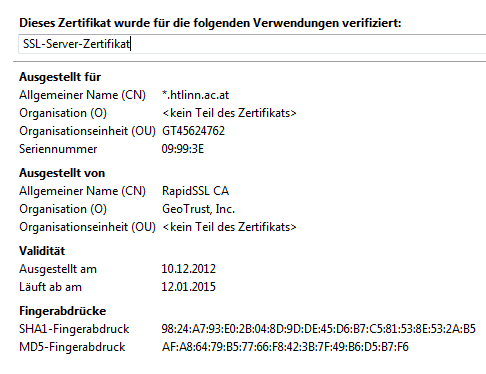
\includegraphics[keepaspectratio=true, width=12cm]{images/screenshots/certificate.png}
\caption{Allgemeine Zertifikatinforamtionen}
\label{fig:certificate}
\end{figure}
Die meisten Browser haben standardmäßig eine Liste von Zertifizierungsstellen eingetragen, welchen sie vertrauen. Diese Liste kann vom User jederzeit erweitert werden, jedoch sollte der User sich bezüglich der Seriosität der Zertifizierungsstelle wirklich sicher sein. 
\paragraph{Extended-Validation-Zertifikat}
Diese Zertifikate wurden entwickelt um eine höhere Sicherheit zu erhalten, als bei \enquote{normalen} Zertifikaten. Dies wird erreicht indem bei der Vergabe genauer kontrolliert wird. \\\\
Wenn bei einer Website ein erweitertes Zertifikat verwendet wird, wird in den meisten Browsern die Adressleiste komplett oder zumindest teilweise grün dargestellt.
\\
Bei der Vergabe dieser Zertifikate werden drei Kriterien besonders beachtet:
Die Identität und die Geschäftsadresse des Auftragstellers, ob der Antragsteller der ausschließliche Eigentümer der Domain ist oder ein exklusives Nutzungsrecht besitzt, ob die antragstellende Person überhaupt befugt ist und ob die rechtlichen Dokumente von zeichnungsberechtigten Personen unterschrieben wurden.

\subsubsection{Sicherheitsprobleme}
Eine Schwachstelle der oben genannten Arten des Schlüsseltausches ist jedoch ein Man-in-the-Middle. Dieser müsste vor Aufbau der Verbindung von Host1 und Host2 zwischen ihnen liegen. In Folge würde er jeweils mit Host1 und Host2 eine Verschlüsselung ausmachen. Wenn er nun die gesendeten Daten von Host1 an Host2 weiterleitet und umgekehrt, können die beiden Hosts dies nicht bemerken.\\
Jedoch benötigt der Man-in-the-Middle ebenso ein Zertifikat, in dem steht, dass er der Zielserver sei. Um dies zu bewerkstelligen, muss der Angreifer Zugang zu einer Zertifizierungsstelle besitzen und sich ein Zertifikat ausstellen lassen.
\subsection{Serverseitige Technologien}
\subsubsection{PHP (Handle)}
Die Abkürzung PHP steht für "PHP Hypertext Preprocessor". Es handelt sich hierbei um ein serverseitige Programmiersprache, die vor allem in der Webentwicklung zum Einsatz kommt. Die Syntax ist an Perl und C angelehnt.\\
Als PHP-Module wurden nur php5-mysql sowie php5-ldap verwendet.\\
PHP ist seit Version 5 vollständig Objekt-orientiert, wurde aber imperativ/funktional verwendet.\\
\\
Ein PHP Programm kann im Gegensatz zu anderen serverseitigen Programmiersprachen direkt in den HTML-Quelltext der Website eingebunden werden. Gekennzeichnet werden diese eingebetteten Programme mit den PHP-Tags (siehe Programm-Code \ref{lst:content_php_Tags}).\\
\begin{lstlisting}[style=custom, language=PHP,  caption={PHP-Tags},label={lst:content_php_Tags}]
<?php 
	/* Programm-Code */
?>
\end{lstlisting}
Befindet sich der PHP Code eingebettet in HTML-Quelltext, so ignoriert der Interpreter alles, das außerhalb der PHP-Tags steht.\\\\
Eines der großen Vorteile an PHP ist, dass es vollständig serverseitig verarbeitet wird, das heißt am Client wird keine Rechenleistung für das Ausführen des PHP-Codes benötigt.
\paragraph{Funktionsweise}
Der Client fragt am Webserver eine Datei mit der Endung .php an. Anschließend lädt der Webserver die Datei und übergibt diese dem PHP Interpreter. Dieser generiert in den meisten Fällen eine HTML Datei, welche anschließend dem Webserver übergeben wird. Dieser sendet die "fertige" Webseite an den Client. (siehe Abb. \ref{fig:content_php_PHP_Funktion}) Der PHP Interpreter ist nicht nur auf HTML Dateien begrenzt, es können auch andere Dateitypen, wie Bilder oder PDF Dateien generiert werden. Diese Funktionsweise hat das Problem, dass die Seite bei jedem neuen Aufruf erneut generiert werden muss, dies führt zu einer höheren Auslastung am Webserver. Um dieses Problem zu vermindern gibt es die Caches am Webserver, die häufig verwendete Programmteile zwischenspeichern, um sie bei erneutem Aufruf nicht erneut Interpretieren zu müssen.
\begin{figure}[H]
\centering
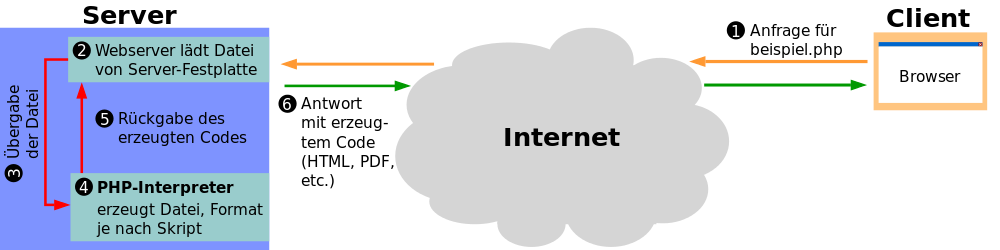
\includegraphics[keepaspectratio=true, width=14cm]{images/PHP_Funktionsweise.png}
\caption{PHP Funktionsweise}
\label{fig:content_php_PHP_Funktion}
\textbf{Quelle:} http://de.wikipedia.org/wiki/PHP
\end{figure}
\paragraph{PHP Sessions}
Mit PHP Sessions kann man einen Besucher einer Webseite über mehrere Aufrufe der Webseite hinweg genau identifizieren. Jedem Besucher auf der Webseite wird eine eindeutige Session-ID zugewiesen, diese wird in einem Cookie auf dem Server abgelegt. Eine PHP Seite, die die Session verwenden soll, muss als erstes des PHP-Dokuments diese Zeile stehen. (siehe Programm-Code \ref{lst:content_php_Session})
\begin{lstlisting}[style=custom, language=PHP, caption={Session},label={lst:content_php_Session}]
<?php
	session_start();
?>
\end{lstlisting}

Damit wird dem Webserver vermittelt, dass diese Seite mit einer Session arbeitet.\\
Die session-ID ist eine 128 Bit lange Zahl die zufällig generiert wird. Diese muss ab nun bei jeder Antwort vom Server an den Client mitgeliefert werden und auch umgedreht. Damit können personenbezogene Informationen einer bestimmten Session zugeordnet werden, wie ein Warenkorb bei Online-Shopping, Status von einer Anmeldung usw. Wir verwenden Sessions um den User über die Webseite hinweg identifizieren zu können. 
\paragraph{Kommunikation mit Server}
PHP hat auch eine Möglichkeit, um diverse Daten dem Server zu 
senden, diese können von der zu empfangenden Webseite verarbeitet werden.\\\\
Diese Funktion wird vor allem bei Formularen eingesetzt, um die User-Interaktion mit der Seite zu steuern. Es wird auch dazu verwendet um auf einer Seite zu navigieren oder ein Login bereitzustellen. Jedoch muss man in diesem Bereich im wesentlichen zwischen 2 Teile unterscheiden:
\begin{itemize}
    \item POST
    \item GET
\end{itemize}
\subparagraph{POST}
Bei POST werden die mitgegebenen Daten nicht an die URL angefügt, wie bei GET, aber dazu später, sondern werden im Body Teil der HTTP/S Anfrage an den Server. (siehe Programm-Code \ref{lst:content_php_HTTP_POST}) Dies hat den großen Vorteil, dass die mitgegebenen Daten praktisch eine unbegrenzte Größe haben können. Dadurch können auch lange Texte, Bilder, Dateien usw. an den Server gesendet werden. Ein weiterer Vorteil liegt darin, dass der User die eingegebenen Daten nicht sieht, d.h. gibt er ein Passwort ein so ist es für ihn nicht einsehbar. Dies schützt jedoch nicht vor Angreifer, die die HTTP Anfragen mitschneiden, deshalb verwendet man beim Senden von Passwörtern immer HTTPS.\\
Im Beispiel Programm-Code \ref{lst:content_php_POST} ist ein kleine Eingabe von einem Text möglich. Bei drücken des Buttons Speichern wird an den Server eine Anfrage gestellt, dass die gleiche Seite nochmals aufgerufen werden sollte, jedoch werden POST Variablen mitgegeben. Diese wertet die Seite mit dem PHP Teil aus und gibt den eingegebenen Text aus. Da dieser Text beliebig lang sein kann, muss POST verwendet werden. Warm siehe Punkt GET.
\begin{lstlisting}[style=custom, caption={Ausschnitt HTTP POST Request},label={lst:content_php_HTTP_POST}]
POST /login/index.php	//Angefragte Seite
HOST sis.htlinn.ac.at	//Host
	//Weitere Informationen
	//Weitere Informationen
	//Weitere Informationen
	//leere Zeile - Trennt Header von Body ab
user=20091234&password=passwort&send=1	//POST-Parameter
\end{lstlisting}
\begin{lstlisting}[style=custom, language=PHP, caption={Beispiel POST},label={lst:content_php_POST}]
<html>
<head>
</head>
<body>
<?php

if(!empty($_POST['text']))	//Wenn die Variable text nicht leer ist
	echo $_POST['text'];	//Soll der Text ausgegeben werden
else	//Wenn sie leer ist
	echo "nichts eingegeben";	//Soll eine Warnung ausgegeben werden
?>

<form method="post">	//method="post" --> Parameter werden mit POST mitgegeben
	<textarea name="text"></textarea>
	<button type="submit" name="save" value="Speichern">
</form>
</body>
</html>
\end{lstlisting}
\subparagraph{GET}
Bei GET werden die mitgegebenen Parameter direkt an die URL angehängt, um dies trennen zu können, wird die Parameterliste mit einem ? eingeleitet. Einzelne Parameter werden mit einem \& getrennt. Diese Methode ist die Standardmethode wenn man ein HTML-Form erstellt. Dies wird bei kleinen Daten verwendet. Der Vorteil liegt darin, dass der User die Seite neu laden kann und die Parameter werden übernommen. Auch kann der User die URL samt den Parametern als Lesezeichen abspeichern, um beispielsweise bei einer Webseite, die die Parameter zur Navigation auf der Seite verwendet, genau die gewünschte Seite zu erhalten. Eine Beispiel-URL sieht wie folgt aus: \textit{sis.htlinn.ac.at/index.php?text=hallo\&send=Speichern}. Dies wäre die URL, die bei absenden des Beispiel Programm-Codes \ref{lst:content_php_GET} entstehen würde. Sofern die Datei des Programm-Codes index.php heißt. Im Prinzip läuft die Auswertung der mitgelieferten Parametern gleich ab, wie bei POST Parametern.\\
Bei GET besteht die Grenze der Datenlänge darin, dass eine URL nur ca. 2000 lang sein darf, dies ist Browser und Server abhängig, aber 2000 Zeichen funktioniert bei allen Server-Client Kombinationen.
\begin{lstlisting}[style=custom, language=PHP,  caption={Beispiel GET},label={lst:content_php_GET}]
<html>
<head>
</head>
<body>
<?php

if(!empty($_GET['text']))	//Wenn die Variable text nicht leer ist
	echo $_GET['text'];	//Soll der Text ausgegeben werden
else	//Wenn sie leer ist
	echo "nichts eingegeben";	//Soll eine Warnung ausgegeben werden
?>

<form method="get">	//method="get" --> Parameter werden mit GET mitgegeben
	<input type="text" name="text"></textarea>
	<button type="submit" name="save" value="Speichern">
</form>
</body>
</html>
\end{lstlisting}
\subparagraph{URL-Encoding}
Die POST und GET Daten die an den Webserver gesendet werden, werden nicht exakt mit den Zeichen übertragen, die man zum Beispiel in ein Textfeld eingibt. Dies hat den Hintergrund, dass einige Zeichen reserviert sind und deshalb nicht in den GET oder POST Daten vorkommen dürfen. Um dies zu verhindern werden diese Zeichen mit anderen ausgetauscht. Dazu wird die Darstellung mit einem \% verwendet. Dabei wird das Zeichen mit der im entsprechendem Hexadezimalen ASCII Code und einem \% ausgetauscht.\\
Also wird die \# durch \%23 ausgetauscht, da die \# die Hexadezimale 23 im ASCII-Code darstellt.\\
Als reserviert gelten die Zeichen ! \# \$ \% \& ' ( ) * + , / : ; = ? @ [ ]. Jedes Leerzeichen wird durch ein + ausgetauscht, welches dann jedoch nicht URL-Codiert wird.
\paragraph{Probleme}
\subparagraph{Typisierung} 
Die Typisierung in PHP ist sehr flexible (dynamisch), so kann einer Variable, die zum Beispiel eine Zahl enthält, 
eine Zeichenkette, oder ein Array neu zugewiesen werden. \\
% typwechsel einer variable ist ja eher ein horror (IMHO)
Manche Standard-Funktionen in PHP haben numerische Rückgabewerte und geben den bool'schen Wert false zurück, 
wenn ein Fehler auftritt. Da alle Werte, die nicht 0 sind, laut Definition gleich dem bool'schen true sind, 
kann es zu Fehlinterpretation des Rückgabewertes kommen. Um solche Situationen so vermeiden, sollte statt auf Wertegleichheit (==) auf Äquivalenz (===), das bedeutet in diesem Zusammenhang Werte- und Typgleichheit (Bool != Integer, trotz dynamischer Typisierung), geprüft werden (Beispiel: siehe Programm-Code \ref{lst:content_php_false}).
\begin{lstlisting}[style=custom, language=PHP,  caption={false},label={lst:content_php_false}]
<?php 
	$string = "Hallo Welt";
	$position = strpos("H", $string); 
	// H liegt an Position 0
	
	// falsch:
	if ($position == false) {
		echo "Abfrage 1\n";
	}
	// richtig:
		if ($position === false) {
		echo "Abfrage 2\n";
	}
?>
\end{lstlisting}
\subparagraph{Serverseitige Realisierung}
Ein Problem und gleichzeitig auch ein Vorteil besteht darin, dass der Webserver die PHP-Datei compiliert 
und eine fertige HTML-Datei an den Client sendet. 
% Das muss er weil der Browser nur HTML versteht.
Der Vorteil liegt darin, dass keine Rechenleistung am Client nötig ist. 
% ausser zum Rendern. Der Vorteil ist, dass Daten angezeigt werden diese aber am Client nicht vorliegen
% z.B. Änderungszeitpunkt einer Datei oder Serveruhrzeit.
Jedoch bedeutet dies auch, dass ohne neue Anfrage zum Server und 
daraus resultierendes Neu Laden der ganzen Seite kann sich nichts am Seitenaufbau ändern. 
% daraus resultierendem Neuladen 
Soll sich z.B. bei Auswählen einer Check Box etwas am Aufbau der Seite ändern, 
so muss entweder die Seite neu geladen werden oder man greift auf andere Technologien zurück. 
(siehe \ref{sec:content_js_Javascript} oder \ref{sec:content_js_AJAX})

\subsubsection{MySQL (Handle)}
MySQL ist eines der bekanntesten und weit verbreitetsten relationalen Datenbankverwaltungssysteme auf der Welt. Ursprünglich wurde es von MySQL AB entwickelt, wurde jedoch von Sun Microsystems übernommen und ist jetzt in Händen von Oracle. Es ist als Open-Source Software oder als kommerzielle Enterprise Version verfügbar.\\
\paragraph{SQL\\}
Dieses Datenbankmanagementsystem verwendet als Sprache für den Zugriff auf die Datenbank SQL.\\
SQL steht für \textbf{Structured Query Language} und wurde dafür entwickelt, eine einheitliche und leicht lesbare Programmierschnittstelle zur Verfügung zu stellen, um Datenbanken zu bearbeiten.\\
SQL ist eine Datenbanksprache für relationale Datenbanken. Sie kann dazu verwendet werden, Datenbanken und Tabellen zu erstellen und bearbeiten, sowie um Datensätze zu bearbeiten - damit ist Löschen, Ändern oder Einfügen von Datensätzen in Tabellen gemeint. Außerdem können auch Datensätze abgefragt, gefiltert, sortiert und vieles mehr werden. Die Voraussetzung ist, dass das Datenbanksystem auf dieser Datenbanksprache basiert.\\
Hier die wichtigsten Befehle die verwendet wurden.\\
\subparagraph{Beispiele für Befehle}
\begin{itemize}
    \item SELECT
    	\begin{itemize}
	    	\item Mit \texttt{SELECT} können Datensätze aus Tabellen abgerufen werden. Zu diesem Befehl gibt es noch einige Zusätze, um zum Beispiel die Daten zu filtern, zu sortieren oder Tabellen miteinander zu verknüpfen.
	    	\begin{itemize}
		    	\item \texttt{SELECT * FROM classes;}\\
		    		Damit werden alle Datensätze aus der Tabelle classes ausgelesen.
		    	\item \texttt{SELECT short FROM teachers;}\\
			    	Damit wird nur die Spalte der Lehrerkürzel ausgelesen, jedoch von allen Datensätzen.
		    	\item \texttt{SELECT * FROM classes WHERE name LIKE '2 \%'}\\
		    		Damit werden alle Datensätze von Klassen ausgelesen, bei denen der Name mit 2 beginnt. So erhält man alle Klassen des 2. Jahrgangs.
		    	\item \texttt{SELECT * FROM substitudes ORDER BY time ASC}\\
		    		Damit werden alle Supplierungen in aufsteigender Reihenfolge(\texttt{ASC}) ausgelesen. Sollen die Supplierungen absteigend ausgelesen werden verwendet man statt \texttt{ASC DESC}.
		    	\item \texttt{SELECT teachers.name FROM classes LEFT JOIN teachers ON \\teachers.ID = classes.teacherFK}\\
		    		Mit dieser Abfrage können alle KV's der Klassen abgefragt werden. Da im Datenbankdesign auf Redundanzvermeidung geachtet wurde, wird in der classes Tabelle auf die teachers Tabelle verwiesen. Dort stehen die Namen der KV's. In der classes Tabelle steht nur die eindeutige ID des Lehrers.\\\\
		    		\textbf{\texttt{SELECT teachers.name FROM classes LEFT JOIN teachers ON \\teachers.ID = classes.teacherFK}}\\
		    			Gibt alle Einträge der Tabelle classes zurück, jedoch nur die Einträge von der teachers Tabelle, welche die \texttt{ON} Bedingung erfüllen.\\\\
		    		\textbf{\texttt{SELECT teachers.name FROM classes INNER JOIN teachers ON \\teachers.ID = classes.teacherFK}}\\
		    			Gibt nur diejenigen Datensätze zurück, welche die \texttt{ON} Bedingung erfüllen.\\\\
		    		\textbf{\texttt{SELECT teachers.name FROM classes RIGHT JOIN teachers ON \\teachers.ID = classes.teacherFK}}\\
		    			Gibt alle Einträge der Tabelle teachers zurück sowie nur die Einträge der Tabelle classes welche die ON Bedingung erfüllen.\\\\
		    		\textbf{\texttt{SELECT teachers.name FROM classes OUTER JOIN teachers ON \\teachers.ID = classes.teacherFK}}\\
		    			Gibt alle Einträge aus beiden Tabellen zurück. Die Einträge, welche die \texttt{ON} Bedingung erfüllen, werden zusammengefügt, und die anderen werden jeweils als einzelner Datensatz angezeigt.\\
		    	\item \texttt{SELECT name as Klassenname FROM classes}\\
		    		Mit as können die Spaltennamen der Tabelle in besser lesbare oder besser identifizierbare Spaltennamen umbenannt werden.
	    	\end{itemize}
    	\end{itemize}
    \item INSERT
	    \begin{itemize}
		   	\item Mit dem INSERT Befehl können neue Datensätze in eine Tabelle eingefügt werden.
		   	\begin{itemize}
			   	\item \texttt{INSERT INTO sections (name, short, teacherFK) VALUES \\('TestAbteilung', 'T', '2')}\\
			   		Damit wird eine neue Abteilung in der Tabelle sections erstellt. Dabei werden die angegebenen Spalten auf die in der Klammer stehenden Werte gesetzt. Hier muss die Spalte ID nicht angegeben werden, da sie auf \textit{auto increment} gesetzt ist.
		   	\end{itemize}
	    \end{itemize}
	\item UPDATE
		\begin{itemize}
			\item Mit dem UPDATE Befehl können Datensätze in einer Tabelle verändert werden.
			\begin{itemize}
				\item \texttt{UPDATE sections SET name = \\'TestAbteilung2' WHERE name = 'TestAbteilung'}\\
					Mit diesem UPDATE Befehl wird jeder Datensatz, der in der Spalte name \enquote{TestAbteilung} stehen hat, abgeändert. Dabei wird \enquote{TestAbteilung} in \enquote{TestAbteilung2} geändert.
				\item \texttt{UPDATE sections SET name = 'TestAbteilung123',short = 'T123' WHERE name = 'TestAbteilung2'}\\
					Dies Funktioniert im Prinzip gleich wie der Befehl zuvor. Mit dem Unterschied, dass dabei 2 Spalten geändert werden.
			\end{itemize}
		\end{itemize}
	\item DELETE
		\begin{itemize}
			\item Mit DELETE können einzelne Datensätze oder auch mehrere Datensätze auf einmal gelöscht werden.
			\begin{itemize}
				\item \texttt{DELETE FROM sections WHERE name = 'TestAbteilung123'}\\
					Damit werden alle Datensätze mit name = TestAbteilung123 gelöscht. Ohne dem WHERE Parameter werden alle Datensätze aus der Tabelle sections gelöscht.
			\end{itemize}
		\end{itemize}
	\item TRUNCATE
		\begin{itemize}
			\item Mit TRUNCATE können alle Datensätze aus einer Tabelle gelöscht werden. Im Unterschied zu DELETE wird hier auch der Index zurückgesetzt. Bei DELETE werden die neuen Datensätze fortlaufend weiter mit dem letzten Index nummeriert. Bei TRUNCATE beginnt die Nummerierung von vorne.
			\begin{itemize}
				\item \texttt{TRUNCATE FROM classes}\\
					Dabei wird die ganze Tabelle classes zurückgesetzt und damit auch alle Datensätze gelöscht. 
			\end{itemize} 
			
		\end{itemize}
\end{itemize}
\paragraph{Aufbau von MySQL}
Bei MySQL ist es im Normalfall so, dass die Datenbank/en auf einem MySQL Server liegen und die MySQL-Client/s Anfragen auf diesen Server senden.\\
Ein Server kann mehrere Datenbanken beinhalten. Eine solche Datenbank kann jeweils mehrere Tabellen beinhalten. Jede Tabelle hat mehrere Spalten.\\
Jede Spalte hat einen bestimmten Datentyp. Hier einige wichtige Datentypen, die benützt wurden:
\begin{itemize}
	\item TINYINT\\
	Wird für die Speicherung von BOOL Werten verwendet, da es den wenigsten Speicherplatz benötigt
	\item INT\\
	Wird für die Speicherung von Ganzzahlen verwendet.
	\item DATE\\
	Wird für die Speicherung von Datumsangaben verwendet.
	\item TEXT\\
	Wird für die Speicherung von Texten verwendet.
\end{itemize}
\paragraph{Verarbeitung von Anfragen}
Eine Anfrage, die an einen MySQL-Server gesendet wurde, wird grundsätzlich mit diesen Schritten abgearbeitet. Zuerst wird im Query-Cache nachgeschaut, ob ein gleicher Query schon einmal gestellt wurde und ob sich die Tabelle seither nicht mehr geändert hat. Ist es ein neuer Query, so wird der Query an den Parser gesendet und anschließend wird der Query optimiert, das Ergebnis wird zurückgeliefert.
\subparagraph{Query-Cache}
Wird ein Query an den MySQL-Server gesendet, wird zuerst im Query-Cache nachgeschaut, ob derselbe Query schon einmal gestellt wurde. Ist dies der Fall, so muss noch kontrolliert werden, ob sich die Daten in der Datenbank seither geändert haben. Hat sich nichts verändert, so sendet der MySQL-Server die gespeicherten Ergebnisse zurück. Dies hat den Vorteil, dass der MySQL-Server nicht wieder den Query ausführen muss und ist somit ressourcensparender. 
\subparagraph{Parsing}
Beim Parsing wird der gestellte Query in seine einzelnen Befehle zerlegt. Außerdem werden alle Informationen über den Query gesammelt. Zum Beispiel wird die Art(SELECT,DELETE,UPDATE,...) des Querys bestimmt. Ist das Parsing abgeschlossen, so ist ein so genannter Parse-Baum erstellt worden. Dieser wird anschließend optimiert.
\subparagraph{Optimierung}
In diesem Schritt wird der geparste Code optimiert. Dabei wird der Query analysiert, so werden die besten Abfragereihenfolgen ausgearbeitet. Es wird bestimmt, welche Tabellen wie und wann gejoined werden. Außerdem wird kontrolliert, ob alle Tabellen, die im Query vorkommen, auch wirklich benötigt werden.\\
Ist die optimale Abfragereihenfolge, gefunden wird der Query ausgeführt und das Ergebnis wird zurückgegeben.
\paragraph{Administration}
MySQL liefert standardmäßig einen Kommandozeilen-Client mit. Dieser kann in der Konsole mit \textit{mysql} aufgerufen werden. Damit können Datenbanken, Tabellen erstellt und bearbeitet werden, Datensätze können bearbeitet, verändert und gelöscht werden. Es können noch viele weitere Funktionen damit genutzt werden.\\
\subparagraph{Grafische Tools}
Es gibt noch zahlreiche grafische Tools, um MySQL Server zu administrieren. Eines der am weit verbreitetsten grafischen Tools ist phpMyAdmin. Dies ist ein Tool, das auf einen Webserver kopiert wird und es erlaubt, über ein Webinterface alle Einstellungen und Datenbankbefehle grafisch auszuführen. Dies erleichtert und vereinfacht das Erstellen, Bearbeiten und Verändern von Datenbanken und Tabellen. Damit können auch ungeübte Personen MySQL Datenbanken verwenden.
\paragraph{MySQL $ \Rightarrow $ PHP}
Um über PHP auf einen MySQL Server zugreifen zu können, benötigt man das PHP-Modul php5-mysql, welches einige Befehle zur Verfügung stellt, um mit einem MySQL-Server zu kommunizieren.\\
\subparagraph{Verbindung aufbauen}
Um mit einem MySQL-Server eine Verbindung aufzubauen müssen diese PHP Befehle verwendet werden(siehe Programm-Code \ref{lst:content_mysql_connect}).
\begin{lstlisting}[style=custom, language=PHP, caption={MySQL Connect},label={lst:content_mysql_connect}]
<?php 
	mysql_connect($host, $user, $passwd);
	mysql_select_db($db);
?>
\end{lstlisting}
In diesem Beispiel entspricht \texttt{\$host} der Adresse des MySQL-Server. \texttt{\$user} ist der Usernamen zum Anmelden auf dem MySQL-Server und \texttt{\$pass} ist das Passwort für die Anmeldung. Mit \texttt{\$db} wird die Datenbank angegeben, mit der gearbeitet werden soll. Die Funktion \texttt{mysql\_connect()} gibt im Fehlerfall \texttt{false} zurück und im Erfolgsfall einen Ressource Wert. \texttt{mysql\_select\_db()} gibt bei Erfolg \texttt{true} zurück, sonst \texttt{false}.
\subparagraph{Anfragen}
Um Anfragen an einen MySQL Server senden zu können, muss man diesen Syntax verwenden(siehe Programm-Code \ref{lst:content_mysql_query})
\begin{lstlisting}[style=custom, language=PHP, caption={MySQL Querys},label={lst:content_mysql_query}]
<?php 
	$sql="SELECT * FROM classes";
	mysql_query($sql);
?>
\end{lstlisting}
In der unter \ref{lst:content_mysql_query} gezeigtem Programmsequenz ist eine Anfrage an den MySQL Server gezeigt. Wichtig ist, dass zuvor die Zeilen vom \autoref{lst:content_mysql_connect} stehen, damit eine Anfrage an den Server gesendet werden kann. \texttt{mysql\_query} gibt bei Datenbankabfragen(\texttt{SELECT}, \texttt{SHOW}, \texttt{EXPLAIN}, ...) das Abfrageergebnis im Erfolgsfall zurück, bei Fehlerfall \texttt{false}. Wird ein anderer Datenbankbefehl(\texttt{INSERT}, \texttt{DELETE}, \texttt{UPDATE}, ...) ausgeführt, so gibt die Funktion bei Erfolg \texttt{true} und bei Misserfolg \texttt{false} zurück.\\
Das Ergebnis ist in Zeilen aufgebaut, d.h. will man jede Zeile abarbeiten, muss man jede Zeile zum Beispiel mit einer do-while-Schleife durchlaufen. Ein interner Positionszeiger verweist auf die momentane Stelle. Die Funktionen zum Abfragen dieser Zeilen stellt den Zeiger immer eine Stelle weiter.\\
Das Ergebnis bei einer Abfrage ist jedoch nicht in einem Format, mit dem man arbeiten kann, deshalb muss dieses Ergebnis noch an weitere Funktionen weitergegeben werden. Hier die von uns am häufigsten verwendeten Funktionen:
\begin{itemize}
	\item \texttt{mysql\_fetch\_array()}
	\begin{itemize}
		\item Mit dieser Funktion wird eine Zeile des Ergebnisses gelesen und in ein Array geschrieben. Zusätzlich wird der Positionszeiger eine Stelle weiter gestellt.\\
		Die Einträge des Arrays werden nummerisch indiziert und sind zusätzlich mit den Spaltennamen referenziert. Das heißt, die Ergebnisse sind in diesem Array doppelt vorhanden.
	\end{itemize}
	\item \texttt{mysql\_fetch\_object()}
		\begin{itemize}
			\item Mit dieser Funktion wird die aktuelle Zeile des Ergebnisses ausgelesen und als Objekt zurückgegeben. Wiederum wird der Positionszeiger eine Stelle weiter gestellt.
		\end{itemize}
	\item \texttt{mysql\_fetch\_row()}
		\begin{itemize}
			\item Diese Funktion gibt eine Zeile des Ergebnisses als Array zurück, das nummerische Indizes hat. Das heißt, hier sind aus dem Array die Spaltennamen nicht ersichtlich. Auch hier wird der Datenzeiger um eine Stelle weiter gestellt.
		\end{itemize}
\end{itemize}
Im Programm-Code \ref{lst:content_mysql_fetch_array} ist ein Ausschnitt einer Abarbeitung eines MySQL Results zu sehen. Hier wird zuerst ein Query an den Server gesendet und danach werden alle Ergebniszeilen durchlaufen und in ein Array gespeichert. Dazu wird \texttt{mysql\_fetch\_array()} verwendet.
\begin{lstlisting}[style=custom, language=PHP, caption={MySQL Query weiterverarbeiten},label={lst:content_mysql_fetch_array}]
<?php 
	$sql = "SELECT * FROM hours LIMIT 0,5"; //Mit LIMIT wird die Abfrage auf die ersten 5 Ergebnisse begrenzt
	$result = mysql_query($sql); //Ergebnis wird in der Variable $result gespeichert
	
	while($row = mysql_fetch_array($result)){	//Jede Ergebniszeile wird durchlaufen
		$ergebnis[] = $row;	//Hier wird die Zeile in einen Eintrag des Arrays geschrieben
	}
	
	print_r($ergebnis);	//Relationale Ausgabe des Arrays mit allen Zeilen
	
?>
\end{lstlisting}
Öffnet man den Quelltext der oberen Seite (Wiederum muss zuvor natürlich der Programm-Code \ref{lst:content_mysql_connect} in dem PHP-Code eingefügt werden, um überhaupt eine Verbindung mit dem MySQL-Server herstellen zu können.), so wird das Array \texttt{\$ergebnis} übersichtlich dargestellt. Das Ergebnis ist in der \autoref{fig:content_mysql_fetch_array} zu sehen.\\
Hier ist gut zu sehen, dass bei \texttt{mysql\_fetch\_array()} die Spalten nummerisch und laut Spaltenname indiziert werden. Dies kann durch den zweiten Parameter in der Funktion \texttt{mysql\_fetch\_array()} geändert werden. Außerdem ist hier zu sehen, dass jede Ergebniszeile einen eigenen Index (nummerisch Nummeriert) in dem Array \texttt{\$ergebnis} hat, daraus ergibt sich ein mehrdimensionales Array.\\
Auf die erste Zeile des Ergebnisses kann also mit \texttt{\$ergebnis[0]} zugegriffen werden. Das Ergebnis dieses Codes ergibt \autoref{fig:content_mysql_fetch_row}. Um dann auf die Start-Uhrzeit der Stunde von der ersten Zeile zugreifen zu können, kann man entweder den nummerischen Index oder die Spaltenbezeichnung verwenden. Also entweder \texttt{\$ergebnis[0][4]} oder \texttt{\$ergebnis[0]['startTime']}.\\ Das Ergebnis dieser Zeilen ist dasselbe, dieses ist in Abb. \ref{fig:content_mysql_fetch_column} zu sehen.\\
\begin{figure}[H]
\centering
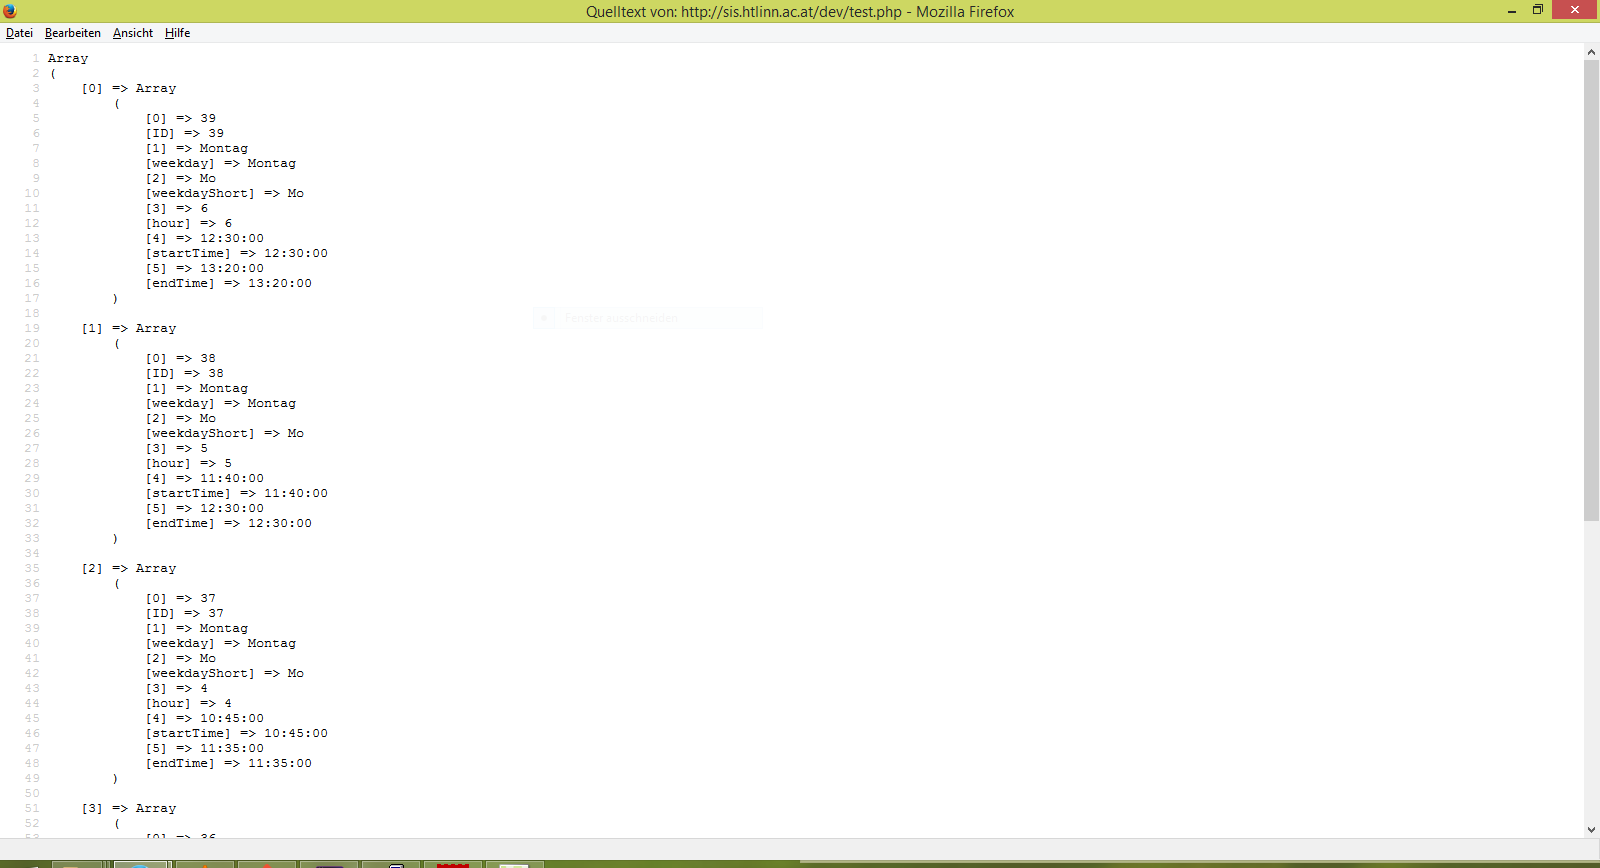
\includegraphics[keepaspectratio=true, width=14cm]{images/screenshots/content_mysql_fetch_array.png}
\caption{MySQL Fetch Array}
\label{fig:content_mysql_fetch_array}
\end{figure}
\begin{figure}[H]
\centering
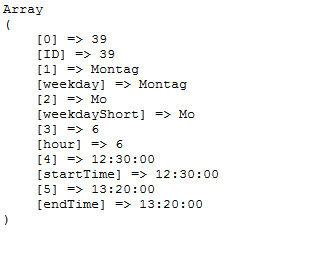
\includegraphics[keepaspectratio=true, width=8cm]{images/screenshots/content_mysql_fetch_row.png}
\caption{MySQL Zeile}
\label{fig:content_mysql_fetch_row}
\end{figure}
\begin{figure}[H]
\centering
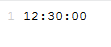
\includegraphics[keepaspectratio=true, width=3cm]{images/screenshots/content_mysql_fetch_column.png}
\caption{MySQL Spalte}
\label{fig:content_mysql_fetch_column}
\end{figure}
\subsubsection{Datenbank-Design (Buchberger)}

Bei relationellen Datenbanken, wie das für das Projekt verwendete MySQL, gelten grundsätzliche Richtlinien, um die Konsistenz der Daten zu gewährleisten:

\begin{description}[style=nextline]
	\item[Entitätsintegrität]
		Die Kennung eines Datensatzes (Primärschlüssel) muss auf jeden Fall eindeutig sein. Dies kann durch die MySQL-Eigenschaft \enquote{auto increment} erreicht werden.
	\item[Referenzielle Integrität]
		Verweise auf andere Tabellen (Fremdschlüssel) müssen auf Datensätze zeigen, die existieren. Alternativ kann NULL zugewiesen werden.\\
		\\
		\textit{Beispiel:} Ein Datensatz für eine Schulstunde hat einen Lehrer, auf den mit einem Fremdschlüssel verwiesen wird. Der Lehrer verlässt die Schule und sein Datensatz wird gelöscht.\\
		\\
		Die Stunde hat weiterhin den gleichen Fremdschlüssel, dessen Datensatz aber nicht mehr existiert.
	\item[Bereichsintegrität]
		Die Werte eines Datenfeldes müssen in einem definierten Bereich liegen.
\end{description}

Weitere wichtige Grundsätze sind:

\begin{description}[style=nextline]
	\item[Redundanzen sind zu vermeiden]
		Anders formuliert: Jede Information soll möglichst nur einmal in der Datenbank vorhanden sein.
		
		Redundanzen sorgen zwangsweise für Probleme, wenn Datensätze aktualisiert werden sollen.
		
		\textit{Beispiel:} Bei einem großen Unternehmen beliefert mehrere Kunden, welche im selben Ort wohnhaft sind. Ändert sich nun die Postleitzahl dieses Ortes, so müssen im Unternehmen alle Datensätze der Kunden aktualisiert werden.
		
		\textit{Lösung:} Auslagern des Ortes und der Postleitzahl in eine weitere Tabelle und via Fremdschlüssel verknüpfen.\\
		So muss bei Änderung der Postleitzahl nur an einer Stelle der Datenbank geändert werden.
		
		Es stellt sich allerdings die Frage, wie weit die Datenstruktur aufgefächert werden soll.
	\item[Gerechnet wird von der Datenbank]
		Das Programm, mit dem die Abfrage an die Datenbank gestellt wird, soll die Daten nicht mehr nachbearbeiten müssen.\\
		Gründe dafür sind, dass die Datenbank für die Verarbeitung von Daten optimiert ist, und dass es beim sequenziellen Abfragen von Tabellen zu Fällen kommen kann, in denen eine Tabelle bereits aktualisiert ist, die verknüpfte Tabelle allerdings nicht.
\end{description}

\subsubsection{LDAP (Buchberger)}

LDAP (Lightweight Directory Access Protocol) ist ein Protokoll für den Zugriff auf Verzeichnis-Datenbanken, wie Microsoft Active Directory, Apple Open Directory, openLDAP oder Novell eDirectory.\\
\\
Verzeichnis-Dienste werden dazu verwendet, um Informationen über Personen oder Rechner-Konfigurationen zu speichern und abzufragen.\\

\paragraph{LDAP-Datenstruktur}

Eine LDAP-Datenstruktur ist Baum-förmig (DIT - Directory Information Tree) aufgebaut.\\
Dies hat den Grund, dass man so geografische und/oder organisatorische Gegebenheiten besser in der Datenbank darstellen kann.
\\
Man unterscheidet zwischen Container-Objekten (enthalten ihrerseits weitere Objekte) und Blatt-Objekten (Sie stellen Enden des Baumes dar).\\
\\
LDAP ist objektorientiert aufgebaut, das heißt, es gibt Objekt-Klassen (wird durch das Schema difiniert), welche Eigenschaften der Objekte vorgeben. Ein LDAP-Objekt besitzt mindestens eine Klasse.\\
\\
Alle Objekte sind durch ihren DN (Distinguished Name) vollständig identifiziert. 
Der DN besteht aus dem Attribut, das das Objekt innerhalb des darüberliegenden Container-Objektes eindeutig macht, zusätzlich zum DN des Container-Objektes.\\
\\
\textit{Beispiel: }\\
uid=mueller,ou=beratung,ou=filliale1,c=at,o=firma\\
\\
Die uid=mueller identifiziert so ein Objekt (vermutlich ein Benutzer) in der ou=beratung. Diese ist wiederum einzigartig in der ou=filliale1, u.s.w.\\
\\
Das lässt sich nun so fortsetzen. Das obestere Container-Objekt wird als Root-Objekt bezeichnet. In den meisten Fällen wird dies mit dem Attribut o (für Organisation) gekennzeichnet.\\
\\
Die Eigenschaften der Objekt sind oft abgekürtzt.\\
\\
\textit{Häufige Abkürtzungen:}\\
\begin{description}[style=nextline]
	\item[o]
		organisationName (Organisation)
	\item[st]
		stateOrProvinceName (Staat/Provinz)
	\item[c]
		country (Land)
	\item[ou]
		organizational unit (Organisations Einheit)
	\item[cn]
		common name (Allgemeiner Name)
	\item[mail]
		e-mail-address (E-Mail-Adresse)
\end{description}

Die Objekt-Klassen definieren die Eigenschaften der Objekt.\\
\\
\textit{Beispiel: } Attribute der Objekt-Klasse inetOrgPerson (Definition des Standard-Schemas initOrgPerson von openLDAP in der Version 1.4.2.6)\\

\begin{description}[style=nextline]
	\item[erbt von]
		organizationalPerson
		\begin{description}[style=nextline]
			\item[erbt von]
				person
				\begin{description}[style=nextline]
					\item[erbt von]
						top	(abstrakte Klasse; keine Attribute)
					\item[!sn]
						sur name (Nachname)
					\item[!cn]
						common name (Allgemeiner Name)
					\item[userPassword]
						Benutzerpasswort
					\item[telephoneNumber]
						Telefon Nummer
					\item[seeAlso]
						Verweiß (als dn)
					\item[description]
						Beschreibung
				\end{description}
			\item[title]
				Titel
			\item[x121Address]
				wurde für das x.121-Protokoll verwendet
			\item[registeredAddress]
				Registrierungs Adresse
			\item[destinationIndicator]
				wurde für Telegram-Services verwendet
			\item[preferredDeliveryMethod]
				Bevorzugte Liefer Methode
			\item[telexNumber]
				wurde für Telex verwendet
			\item[teletexTerminalIdentifier]
				wurde für Teletex verwendet
			\item[telephoneNumber]
				Telefon Nummer
			\item[internationaliSDNNumber]
				ISDN Nummer
			\item[facsimileTelephoneNumber]
				Fax Nummer
			\item[street]
				Staßen Adresse
			\item[postOfficeBox]
				Postfach
			\item[postalCode]
				Postleitzahl
			\item[postalAddress]
				Post Adresse
			\item[physicalDeliveryOfficeName]
				Postbüro Name
			\item[ou]
				organisation unit (Organisations Einheit)
			\item[st]
				stateOrProvinceName (Staat/Provinz)
			\item[l]
				localityName (Ort/Ortschaft)
		\end{description}
	\item[audio]
		Audio
	\item[businessCategory]
		Geschäfts-Kategorie
	\item[carLicense]
		Fahrzeug-Lizenz
	\item[departmentNumber]
		Abteilung innerhalb eines Unternehmens
	\item[displayName]
		bevorzugter Anzeigename
	\item[employeeNumber]
		Angestellten Nummer
	\item[employeeType]
		Anstellungsart
	\item[givenName]
		Vorname(n)
	\item[homePhone]
		Heim-Telefon-Nummer
	\item[homePostalAddress]
		Heim-Andresse
	\item[initials]
		Initialen
	\item[jpegPhoto]
		JPEG Foto
	\item[labeledURI]
		Uniforme Resourcen ID mit optimaler Bezeichnung
	\item[mail]
		e-mail-address (E-Mail-Adresse)
	\item[manager]
		dn des Managers
	\item[mobile]
		mobile Telefon-Nummer
	\item[o]
		organisationName (Organisation)
	\item[pager]
		Telefon-Nummer des Pagers
	\item[photo]
		Foto
	\item[roomNumber]
		Raum Nummer
	\item[secretary]
		dn des Sekretärs
	\item[uid]
		Benutzer Kennung
	\item[userCertificate]
		Beuntzer Zertifikat		
	\item[x500uniqueIdentifier]
		ID für das X.500 Protokoll
	\item[preferredLanguage]
		bevorzugte Sprache
	\item[userSMIMECertificate]
		SignedData für S/MIME
	\item[userPKCS12]
		PKCS \#12 PFX PDU für den Austausch von persönlichen Identitäts-Informationen
\end{description}

\paragraph{LDAP-Suche}

Für die Suche in einer LDAP-Datenstruktur wird als erstes ein baseDN festgelegt, dieser entspricht dem Objekt, ab dem im Baum gesucht werden soll. Weiters wird der Scope festgelegt, hierbei gibt es 3 verschiedene Möglichkeiten:

\begin{description}[style=nextline]
	\item[base]
		Hierbei wird nur das Objekt mit dem baseDN durchsucht.
	\item[one]
		Eine Ebene unterhalb des baseDN wird gesucht.
	\item[sub]
		Alle darunter liegende Objekte sowie das, durch den baseDN referenzierte, werden durchsucht.
\end{description}
Die Suchkriterien werden in der Polnischen Notation (Präfixnotation) geschrieben und dürfen Wildcards enthalten.\\
\\
\textit{Beispiel:}\\
baseDN: ou=STUDENTS,o=HTLinn\\
scope: sub\\
(\&(l=5*H*)(mail=Andreas*)(cn=2009*))\\
\\
Diese Suchanfrage würde alle Objecte liefern, die
\begin{itemize}
	\item
		unterhalb von ou=STUDENTS,o=HTLinn liegen 
	\item	
		und die die Eigenschaften mail, l und cn enthalten
	\item	
		und bei denen der cn mit 2009 beginnt 
	\item	
		und deren E-Mail-Adresse mit Andreas beginnt 
	\item	
		und deren Ort-Attribut mit 5 beginnt und ein H enthält.
\end{itemize}
\subsection{Clientseitige 
Technologien}
\subsubsection{HTML (Weiland)}

HTML steht für "'Hypertext Markup Language"' und bezeichnet eine Auszeichnungssprache. HTML-Dateien werden hauptsächlich für Websites verwendet.


\paragraph{Aufbau}

Eine HTML-Datei ist grundsätzlich immer gleich aufgebaut. Sie besteht aus einem Header in dem unter anderem der Titel und die Meta-Daten bestimmt werden.
Im Body steht der Inhalt der Datei, welcher angezeigt werden soll. 
\begin{lstlisting}[style=custom, language=HTML, caption={HTML-Tags}]
<!DOCTYPE html>
<html> 
	<head>
		/* Datei-Kopf */
	</head>
	<body>
		/* Inhalt der Datei */
	</body>
</html>
\end{lstlisting}

\paragraph{HTML5}
HTML5 ist die aktuellste Version von HTML. Die Entwicklung begann am 29. April 2009 und soll im Jahr 2014 fertiggestellt werden.\\
Mit der Einführung von HTML5 kommen viele neue Elemente, wie zum Beispiel \enquote{details} und \enquote{summary}, zum HTML-Standard dazu. Dies Elemente sind zum Teil interaktiv, was im bisherigen Standard nicht möglich war. So wird zum Beispiel mit dem Element \enquote{details} eine Ausgabe erzeugt die ein-oder ausgeklappt werden kann ohne ein Script zu verwenden oder eine serverseitge Aktion zu erfordern.\\
Im Gegensatz zu früheren Versionen von HTML wird die Wiedergabe von Video- und Audiodateien unterstützt. Jedoch sind aktuell noch nicht alle Browser fähig, diese Funktionen zu verwenden.\\
Die unterstützten Formate sind für Videodateien 0gg Theora, MP4(H.264) und WebM(VP8) und für Audiodateien 0gg Vorbis, MP3 und Wav. \\
\begin{description}[style=nextline]
\item[in SIS verwendete Funktionen:]
\item[datalist] Liste von <option> Elementen, welche von anderen Elementen verwendet werden kann. Unter anderem verwendet um bei der Auswahl des angezeigten Stundenplans eine vorgefertigte Liste der Klassen und Lehrkräfte zu verwenden.
\item[video] Gibt ein Video aus. Bei uns wurde der Befehl (CODE EINFÜGEN) verwendet. Wobei die Option \enquote{autoplay} angibt ob das Video bei einem Seitenaufruf automatisch starten soll und die Option \enquote{loop} ob die Wiedergabe in einer Endlosschleife laufen  soll.
\item[source] Wird bei video und audio verwendet um verschiedene Quellen anzugeben. Somit verwendet jeder Browser die Quelldatei, welche er bevorzugt. Diese Option wurde bei der Wiedergabe des Videos verwendet, wobei als \enquote{src} der Speicherort des Videos und als \enquote{type} der Typ (z.B. video/mp4) der Datei verwendet werden muss. 
\end{description}
\subsubsection{Javascript (Klotz)}
\label{sec:content_js_Javascript}
JavaScript ist eine Skriptsprache welche für dynamische Erweiterungen im Webbrowser gedacht war. Es sollte helfen interaktive Websites, einfacher zu erstellen. Daher ist JavaScript auch nicht als alleinstehende Programmiersprache geeignet, und kommt fast immer in Kombination mit anderen Programmen oder Programmiersprachen zum Vorschein.\\
JavaScript wird hauptsächlich Clientseitig, das heißt im Webbrowser des Nutzers, genutzt um für den Nutzer Extras einzubauen. Dadurch wird auch der Server entlastet, da die Rechenleistung des Anwender-PCs genutzt wird und nicht die des Servers.\\
 Es gibt aber auch Serverseitiges-JavaScript(SSJS). Das kann dann, mit einem entsprechenden Interpreter (z.B.: Node.js), gleich wie andere Serverseitige Programmiersprachen verwendet werden.\\
JavaScript ist, wie die meisten Skriptsprachen, sehr einfach gehalten und Variablendeklarationen und ähnliches fallen weg(Variablentypen können auch während Laufzeit einfach verändert werden).\\
JavaScript ist eine Interpreter-Programmiersprache, das heißt, dass der Code erst im Webbrowser durch den integrierten Interpreter umgesetzt wird.\\
Obwohl JavaScript eine sehr einfache Programmiersprache ist, sind trotzdem alle wichtigen Strukturelement, wie Schleifen, If-Klauseln, etc. welche auch in anderen Programmiersprachen wie zum Beispiel C oder Java existieren, enthalten.\\
Weiters gibt es bei JavaScript die Möglichkeit Bibliotheken einzubinden. Dadurch kann man bereits vorgefertigte Funktionen einfach einbinden und anwenden. Ein Beispiel dafür ist JQuery.\\

\paragraph*{Anwendung}
Um JavaScript in einer Webseite zu nutzen gibt es zwei Möglichkeiten, entweder der Code wird direkt in das HTML-Dokument geschrieben(Variante1) oder man schreibt den JavaScript-Code in ein eigenes Dokument und bindet dieses dann ein(Variante2).\\
Variante 1\\
Wenn man den Code direkt in die HTML-Datei schreiben möchte, muss dieser Code dementsprechend markiert werden. Dazu verwendet man den Script-Tag (siehe Codebeispiel), dieser kann im Head oder im Body stehen, es ist jedoch üblich Funktionen in den Head zu schreiben.\\
\begin{lstlisting}
<html>
  <head>
    <script>
	//Here comes JS
    </script> 
  </head>
  
  <body>
  </body>
</html>
\end{lstlisting}


Variante 2\\
Im Gegensatz zur ersten Variante kommt in diesem Fall nur die Verlinkung zur JavaScript-Datei und nicht der ganze Code in das HTML-Dokument. Das eingebundene JavaScript-Dokument muss nicht auf dem gleichen Server oder Rechner gespeichert sein wie die Webseite, der Code kann sogar aus dem Internet geladen werden. Zum Einbinden einer JavaScript-Datei wird wieder ein Script-Tag verwendet, diesmal wird aber die URL der JavaScript-Datei als Attribut(„src = “) mitgegeben.\\
\begin{lstlisting}
<script src="js/jquery.js" type="text/javascript"></script>
\end{lstlisting}

\paragraph*{Funktionen}
In JavaScript kann man auch Funktionen schreiben, welche dann bei eintreten bestimmter Ereignisse ausgeführt werden. Der Code für eine JavaScript-Funktion sieht wie folgt aus:\\
\begin{lstlisting}
function functionname()
{
some code to be executed
}
\end{lstlisting}
Zwischen den geschwungenen Klammern wird der Code, der ausgeführt werden soll, geschrieben.\\
Um eine Funktion aufzurufen schreibt man den Funktionsnamen mit Klammern dahinter. Der Funktionsaufruf kann zwischen zwei Script-Tags geschrieben werden oder als bestimmtes Attribut (z.B. „onClick“) in manchen anderen Tags.\\
Bei einem Funktionsaufruf kann man der Funktion auch Werte mitgeben, dazu muss man in der Klammer hinter dem Funktionsnamen die Werte/Variablen eintragen. Die Mitgabe von Parametern muss natürlich in der Funktion vorgesehen werden, ansonsten werden die Werte einfach ignoriert.\\

\paragraph*{Variablen}
Bei JavaScript gibt es, wie auch bei anderen Programmiersprachen, Variablen. Diesen muss aber im Gegensatz zu Programmiersprachen wie C, Java oder ähnlichen, bei der Deklaration, kein eindeutiger Variablentyp zugewiesen werden. In JavaScript nur zwei Unterscheidungen bei den Variablentypen, nämlich in Zahlen und in Zeichen bzw. Zeichenketten. 
Um in JavaScript eine Variable zu deklarieren, schreibt man var und dann den Variablennamen. Um ihr dann noch einen Wert zuzuweisen muss man nur den Variablennamen und ein = Symbol schreiben, danach wird der gewünschte Wert hingeschrieben, falls es sich um eine Zeichenkette handelt muss man den Wert zwischen Anführungszeichen setzen:\\
\begin{lstlisting} 
var name = “Peter”;
var Anzahl;
Anzahl = 3;
name = "Hans";
\end{lstlisting}

Weiters muss man zwischen globalen und lokalen Variablen unterscheiden, während globale Variablen im gesamten Dokument definiert sind, sind lokale Variablen nur in der Funktion in der sie deklariert werden nutzbar. Um eine Variabel global zu definieren muss sie außerhalb jeglicher Funktionen definiert werden, wenn man eine Variabel aber innerhalb einer Funktion definiert handelt es sich um eine lokale Variable.\\

\paragraph*{Arrays}
In JavaSript gibt es auch Felder(Arrays). In diesen Feldern können sowohl Zahlen als auch Zeichen bzw. Zeichenketten gespeichert werden, es ist sogar möglich Zahlen und Zeichenketten in dasselbe Array zu speichern.\\
Einen Wert in einem Array zu speichern funktioniert gleich, wie einer Variable einen Wert zuzuweisen, aber bei einem Array muss man zusätzlich zum Arraynamen noch die angeben welchen Arrayeintrag man verändern möchte.\\
\begin{lstlisting}
var cars = new Array();
cars[0] = "Audi";
cars[1] = "BMW";
cars[2] = "Mercedes";
\end{lstlisting}

\paragraph*{JSON}
JSON (JavaScript Object Notation) ist ein Datenaustauschformat welches so gestaltet ist, dass Menschen es leicht lesen können und der Computer es einfach parsen kann. Es basiert auf JavaScript.\\
JSON wird sehr häufig in Verbindung mit JavaScript verwendet, kann aber auch mit anderen Programmiersprachen verwendet werden.\\
Beispiel für ein JSON-Objekt:\\
\begin{lstlisting}
{
  "Gerät": "Auto",
  "Marke": "Audi",
  "Farbe": "rot",
  "Seriennummer": 02345032,
}
\end{lstlisting}

Die Daten werden in Form von Daten-Wert Paaren gespeichert. Aus diesem Objekt kann man nur relativ einfach Daten auslesen. Der JavaScript-Code um die Marke auszulesen würde zum Beispiel wie folgt aussehen:
var Marke = object.Marke;


\subsection{Mobil App (Klotz)}

\subsubsection{PhoneGap}
PhoneGap ist ein Framework, von Adobe Systems, um mobile Apps zu erstellen. Diese Apps sind jedoch weder Web-Apps noch native Apps. Hierbei handelt es sich um Hybrid-Apps. Das heißt die App verwendet nicht die nativen Userinterface Frameworks um das Layout zu gestalten, sondern Web-Technologien, aber die App arbeitet trotzdem vollkommen lokal auf dem Gerät.\\
Das funktioniert indem die App praktisch im Webbrowser des eigenen Gerätes ausgeführt wird, aber alle browsertypischen Eigenschaften, wie zum Beispiel der Rahmen, die URL-Leiste oder die Einstellungen deaktiviert oder ausgeblendet werden.\\
Im Gegensatz zu herkömmlichen Web-Applikationen, kann man mit PhoneGap-Apps auch auf Funktionen wie zum Beispiel den Beschleunigungssensor oder die Kamera zu nutzen. Das wird durch die PhoneGap API ermöglicht. Dabei handelt es sich um Java-Dateien die bei der Installation der App heruntergeladen werden. Mit JavaScript kann man dann über diese Java-Dateien auf die Geräteinternen Sensoren zugreifen. Es handelt sich hierbei also um einen Kompromiss aus Web-Entwicklung und nativer App-Entwicklung.\\
Um PhoneGap zu nutzen muss man sich für alle Systeme, auf denen die App nach der Entwicklung betrieben werden soll, ein SDK installieren, zum Beispiel für Android Eclipse, für iOS XCode oder für WindowsPhone das Microsoft SDK. In dieses SDK muss nun PhoneGap als Plugin geladen werden und mit diesem Plugin kann man die App auch mit Webtechnologien (HTML, CSS, JS) anstatt gerätespezifischer Programmiersprachen (Java, ObjectiveC, VisualC) entwickeln.\\
Unterstützte mobile Betriebssysteme bis Version(2.9):\\
					Android\\
					IOS\\
					Windows Phone 7 \& 8\\
					Blackberry\\
					WebOS(HP)\\
					Tizen\\
					Symbian\\
					Bada\\
Ab PhoneGap-Version 3.0 werden nur noch Android, iOS und Windows Phone unterstützt.\\

PhoneGap basiert auf dem Open-Source-Projekt Apache Cordova. Daher darf PhoneGap auch vollkommen kostenlos genutzt werden.\\
\paragraph{PhoneGapBuild\\}
Für dieses Projekt wurde PhoneGapBuild verwendet.\\
Bei PhoneGapBuild handelt es sich um eine Online-Variante von PhoneGap. Diese wird von AdobeSystems kostenlos zur Verfügung gestellt. Der Vorteil dieser Variante ist, dass nicht für jedes Betriebssystem, für das die App entwickelt werden soll, eine eigene SDK installiert werden muss, da die Applikation direkt online kompiliert wird.\\
Den Code kann man entweder in Form einzelner HTML-, CSS-, und JS-Dateien verpackt als ZIP-Datei hochladen, oder ein GitHub Projekt angeben in dem sich der Code befindet.\\
Nach dem Hochladen des Codes wird die App online sofort kompiliert und die Installationsdateien(APK, XPA, etc.) werden als Download zur Verfügung gestellt.\\

Für die App-Entwicklung mit PhoneGapBuild benötigt man ausschließlich einen Editor und einen Webbrowser, da es sich ja eigentlich um Webentwicklung handelt. Die App besteht nur aus einer(oder mehreren) Webseite(n), welche mit CSS gestaltet wird. Um die Applikation interaktiv zu gestalten, kann man mit JavaScript-Skripts arbeiten und diese auch integrieren. Im Gegensatz zur Webentwicklung gibt es bei der App zusätzlich noch eine Datei mit dem Namen config.xml. In dieser Datei stehen alle Informationen, wie zum Beispiel die Versionsnummer oder der Name, zu der App und anhand dieser Datei können Berechtigungen für den Zugriff auf das Gerät vergeben werden.\\

\subsubsection{iOS}
iOS ist das mobile Betriebssystem von Apple, es wird nur auf IPhones und IPads betrieben. Das Betriebssystem basiert auf dem MacOSX-Kern und somit auch auf einem Unix-Kern.\\
Mit iOS vermarktet Apple den größten Konkurrenten von Android, obwohl das System nur auf den eigenen Geräten installiert wird, ist iOS das am 2. häufigsten genutzte mobile Betriebssystem mit ca. 13\% Marktanteil.\\
\paragraph*{Appstore\\}
IPhone- bzw. IPad-User können Applikationen für ihre Geräte im Appstore herunterladen.\\ 
Eine Besonderheit an iOS ist, dass Apps ausschließlich aus dem Appstore geladen werden können. Das soll mehr Sicherheit und Kontrolle bieten.\\
Um eine Applikation in den Appstore zu laden muss man Developer sein, wofür man wieder um jährlich 99\$ zahlen muss. Für das Veröffentlichen selbst muss man aber keine weiteren Gebühren bezahlen, aber Appel bekommt ca. 30\% der Einnahmen wenn die App kostenpflichtig ist.\\
\paragraph*{PhoneGap mit iOS\\}
Im Laufe des Projekts wurde eine Möglichkeit gefunden den Appstore zu umgehen. Wenn man eine iOS-Applikation mit dem Dienst „PhoneGap Build“ von Adobe erstellt, benötigt man zwar die geeigneten Zertifikate von Apple, das heißt man muss trotzdem als Developer angemeldet sein und jährlich 99\$ bezahlen, aber wenn man nun mit dem IPhone oder IPad dem Downloadlink folgt kommt anstatt des üblichen Downloads die Frage ob man die App installieren will.
Wenn es sich bei den ausgestellten Zertifikaten um Distribution-Zertifikate handelt, ist es so möglich die App auf allen iOS-Geräten zu installieren ohne sie in den Appstore zu stellen. Um diese Funktion zu ermöglichen wurde wahrscheinlich ein Abkommen zwischen Apple und Adobe geschlossen.\\

\subsubsection{Android}
Android ist ein Betriebssystem für Smartphones, welches von Google entwickelt wird. Es basiert auf einem Linux-Kernel.\\
Bei Android handelt es sich um das am weitesten verbreitete mobile Betriebssystem, es hat einen Marktanteil von ca. 80\%. Es wird als freie Software gehandelt und wird als Open-Source entwickelt.\\
\\
\paragraph*{Architektur\\}
Android baut wie bereits erwähnt auf einem Linux-Kernel auf.  Dieser stellt eine Schnittstelle zwischen der Hardware und der höher gelegenen Software dar.\\
In der nächsthöheren Systemschicht sind Android-Klassenbibliotheken, durch welche man die Funktionen des Kernels nutzen kann. Zusätzlich befindet sich auf dieser Ebene eine Dalvik-Virtual-Machine, dabei handelt es sich um eine virtuelle Maschine in der die Applikationen ausgeführt werden.\\
Diese virtuelle Maschine wurde von Google entwickelt und ähnelt in ihrer Funktionalität sehr der Java-VM. Die virtuellen Maschinen führen den Bytecode der Applikationen aus, aber die Dalvik Maschine arbeitet als Registermaschine, weshalb normaler Java-Bytecode auf Android nicht funktioniert.\\
Android startet für jede gestartete Applikation eine eigene virtuelle Maschine, dadurch kann keine App direkt auf das System zugreifen sondern nur über die virtuelle Maschine und des weiteren können sich die Apps nicht gegenseitig stören oder beeinflussen, dadurch dass sie in verschiedenen virtuellen Maschinen betrieben werden.\\
\\
\paragraph*{Store\\}
Im Google Play Store sind viele Apps für Android verfügbar. Dieser Store ist komplett kostenlos nutzbar, jedoch gibt es kostenpflichtige Applikationen. Um Apps aus dem Play-Store zu installieren muss man aber einen Google-Account besitzen welcher auch komplett kostenlos ist.\\
Bei Android kann man den Store relativ einfach umgehen, denn bei Android kann man alle APK-Files(Android-Installationsdateien) einfach ausführen. Dazu muss man nur in den Einstellungen im Menü Anwendungen, den Punkt Unbekannte Quellen aktivieren. Damit erlaubt man das Installieren von Apps die nicht aus dem Play-Store heruntergeladen werden.\\
Ist das erledigt muss man nur noch das gewünschte APK-File auf dem Smartphone speichern (downloaden oder über USB auf dem Smartphone speichern) und dieses dann öffnen. Dann wird die Applikation automatisch installiert und ist danach wie jede andere Applikation auf dem Gerät installiert.\\
 Um Apps in den Play-Store hochzuladen muss man als Entwickler registriert sein. Eine Registrierung als Entwickler kostet einmalig(Registrierungsgebühren) 25\$. Nach dieser Registrierung kann man kostenlos so viele Apps hochladen wie man will, bei kostenpflichtigen Apps verlangt Google jedoch ca 30\% der Einnahmen.\\



\subsubsection{Windows Phone}

\subsubsection{Sonstiges}

\subsection{Sicherheitsprobleme}
\subsubsection{MySQL-Injection (Handle)}
Mit SQL Injections versucht ein Angreifer Daten aus der Datenbank auszulesen, Daten zu manipulieren und noch einige weitere Dinge, die nicht im Auge des Programmierers liegen, zu machen. Diese Injections sollen natürlich so gut es geht vom Programmierer verhindert werden, dazu stellt PHP einen Befehl zur Verfügung. Dieser lautet: \textit{mysql\_real\_escape\_string()}.
\paragraph{Beispiele}
Bei dem Programm-Code \ref{lst:content_mysql_sql_injection_1} ist gezeigt wie eine Injection erfolgreich durchgeführt werden kann. Dabei wird bei einer einfachen Anmeldung die Anmeldung ausgetrickst und man kann sich ohne Passwort anmelden.
\begin{lstlisting}[style=custom, language=PHP, caption={MySQL Injection: Falsch},label={lst:content_mysql_sql_injection_1}]
<?php 
	$sql = "SELECT * FROM users	WHERE name='$_POST['username']' AND password='$_POST['password']'";	//Die mitgegebenen Werte werden in den Query übernommen
	mysql_query($sql);	//Query wird ausgeführt
	
?>
\end{lstlisting}
Sofern der User wirklich einen regulären Benutzername und einen reguläres Passwort eingibt macht diese Vorgangsweise keine Probleme.\\
Nehmen wir jetzt an, dass der User ein Angreifer ist und sich ohne ein Passwort zu kennen zugriff zum Passwortgeschützten Bereich machen will, dann macht der Programm-Code \ref{lst:content_mysql_sql_injection_1} Probleme.\\
Beispiel:\\
\begin{itemize}
	\item \$\_POST['username'] = 'asdf'\\
	Dieser Benutzername muss nicht existieren in der Datenbank
	\item \$\_POST['password'] = "' OR ''=''"\\
	Damit wird ein Ausdruck angefügt der immer 1 ergibt
\end{itemize}
$ \rightarrow $ \textit{SELECT * FROM users WHERE name='asdf' AND password='' OR ''=''}\\
Mit dieser Eingabe eines Angreifers bekommt man bei diesem Select Query immer ein Ergebnis zurück. Welches, kommt drauf an wie es ausgewertet wird, zum erfolgreichen einloggen führen kann. Dies kann mit dem oben erwähnten Befehl verhindert werden. Siehe Programm-Code \ref{lst:content_mysql_sql_injection_2}
\begin{lstlisting}[style=custom, language=PHP, caption={MySQL Injection: Richtig},label={lst:content_mysql_sql_injection_2}]
<?php 
	$user = mysql_real_escape_string($_POST['username']);
	$paswd = mysql_real_escape_string($_POST['password']);
	$sql = "SELECT * FROM users WHERE name='$user' AND password='$paswd'";	//Die kontrollierten Werte werden in den Query Übernommen
	mysql_query($sql);	//Query wird ausgeführt
	
?>
\end{lstlisting}
Geht man davon aus, dass die selben Werte vom Angreifer eingegeben werden, so kommt es jetzt nicht zu einem Ergebnis, da die Funktion alle nicht erlaubten Zeichen 'eliminiert'. Sie werden nicht direkt eliminiert, sondern die nicht erlaubten Zeichen werden nicht gelöscht, sondern mit einem \textbackslash maskiert. Also aus einem \textit{'} wird ein \textit{\textbackslash'}, aus einem \textit{"} wird ein \textit{\textbackslash"} usw. Die Zeichen, die mit einem Backslash maskiert werden, sind ",',\textbackslash n,\textbackslash r,\textbackslash,\textbackslash x00,\textbackslash x1a.\\
Es können nicht nur wie oben gezeigt SELECT-Befehle verändert werden, sondern es können ganze Befehle in Befehle eingefügt werden. Dadurch kann ein Angreifer zum Beispiel einen neuen Datensatz anlegen, Datensätze löschen und so weiter.
\begin{lstlisting}[style=custom, language=PHP, caption={MySQL Injection: Beispiel Query in Qeury},label={lst:content_mysql_sql_injection_3}]
<?php 
	$ID = $_GET['ID'];
	
	$sql = "SELECT * FROM users	WHERE ID={$ID}";
	mysql_query($sql);	//Query wird ausgeführt
	
	//Mitgegebener GET Wert = 2
	//Query : SELECT * FROM users	WHERE ID=2
	
	//Mitgegebener GET WERT = 2;UPDATE users SET type="admin" WHERE ID=23
	//Query : SELECT * FROM users	WHERE ID=2;UPDATE users SET type="admin" WHERE ID=23
	//Damit kann zum Beispiel einem User eine andere Berechtigung gegeben werden
?>
\end{lstlisting}
Im \autoref{lst:content_mysql_sql_injection_3} ist gezeigt wie ein Angreifer zum Beispiel einem beliebigen User die Berechtigungen admin gebem kann. Was natürlich eine sehr große Sicherheitslücke darstellt. Dies kann wiederum mit der Funktion \textit{mysql\_real\_escape\_string()} verhindert werden.
\subsubsection{Cross-Site Scripting (Weiland)}
Oft auch XSS genannt. Bei einem Angriff mit Cross-Site-Scripting wird eine Website, welche auch eine ansonsten vertrauenswürdige Seite sein kann, vom Angreifer mit einem Script versehen, welches im Browser des Opfers ausgeführt wird.\\
Dabei muss der Angreifer nicht zwangsläufig auf den Server zugreifen können. Dadurch, dass viele Seiten dynamisch gestaltet sind, bieten sich einem Angreifer viele Möglichkeiten. Zum Beispiel gibt es oft die Möglichkeit eine Kommentar zu hinterlassen. Wenn in solch einem Feld ein Script platziert wird, wird es vom Browser eines Betrachters automatisch ausgeführt.
\paragraph{Problem}
Es gibt grundsätzlich drei verschiedene Arten von Cross-Site-Scripting:
\subparagraph{reflektiert oder nicht-persistent}
Bei dieser Art des XSS wird das Script vom Benutzer \enquote{geliefert} und nicht auf dem Server gespeichert. Die ist zum Beispiel möglich, wenn wie bei \autoref{lst:content_XSS_Vulnerable} eine vom Benutzer getätigte Eingabe direkt ausgegeben wird. Dies kann ebenso über GET- oder POST-Methoden funktionieren. So kann ein Angreifer einem Opfer mit dem Link zu der Seite und einem angefügten Script als z.B GET-Parameter (z.B. \texttt{input=<script type="text/javascript"> alert ('Dies sollte nicht passieren!'}) dazu bringen ein Script auszuführen
\subparagraph{persistent oder beständig}
Bei dieser Vorgehensweise wird das Script auf der Website gespeichert und somit bei jeder Anfrage ausgeliefert wird.\\ Dies lässt sich leicht anhand eines Forums beschreiben:\\\\
Der Angreifer hinterlässt eine Nachricht im Forum, in der ein Script eingebaut ist. Sobald nun ein Besucher des Forums diese Nachricht lesen will, führt der Browser das Script aus.
\subparagraph{DOM-basiert oder lokal}
Diese...
\begin{lstlisting}[style=custom, language=PHP, caption={Cross-Site-Scripting Anfällig},label={lst:content_XSS_Vulnerable}]
<html>
	<head>
	<title> Cross-Site-Scripting</title>
	</head>

	<body>
		<?php
		if(isset($_GET['input'])) echo $_GET['input'];
		else echo "keine Eingabe get&auml;tigt";			
		?>
	</body>
</html>
\end{lstlisting}




\paragraph{Methoden um Vorzubeugen}

Um XSS auf seiner eigenen Site zu verhindern sollten alle Eingaben, welche ausgegeben werden zum Beispiel mit dem Befehl \enquote{htmlspecialchars} behandelt werden. Dadurch werden alle Sonderzeichen durch die dafür vorgesehenen html-Zeichen umgewandelt (aus < wird \&lt;), wodurch kein ausführbares Script mehr vorliegt.

Manche Browser verhindern die Verwendung von XSS automatisch, so wird beispielsweise bei Internet Explorer 11 diese Meldung (\autoref{fig:content_security_xss_ie}) ausgegeben, wenn die Seite \autoref{lst:content_XSS_Vulnerable} mit einem Script als input aufgerufen wird.

\begin{figure}[H]
\centering
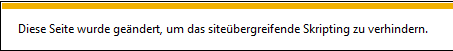
\includegraphics[keepaspectratio=true, width=14cm]{images/screenshots/xss_ie.png}
\caption{Internet Explorer blockiert XSS}
\label{fig:content_security_xss_ie}
\end{figure}
\subsubsection{Cross-Side Request Forgery (Buchberger)}
\label{sec:content_security_xsrf}
\paragraph{Problem\\}
Folgende Situation:\\
Ein Super-Admin (nennen wir ihn Bob) ist in SIS eingeloggt, solange er das Browser-Fenster nicht schließt, bleibt die PHP-Session aufrecht. \\
Nun öffnet er in einem anderen Browser-Tab versehentlich die Website von Marvin (Marvin kennt die SIS-Seite, und er kennt den Source-Code). Marvins Seite fragt mit AJAX die SIS-Seite an. Er füllt mit JavaScript das Formular zum Löschen der Stundenpläne aus und sendet es zurück. Da diese Anfrage mit Bobs Webbrowser ausgeführt wird, und dieser eine offene PHP-Session mit SIS hat, glaubt das SIS-System, dass die Anfrage von Bob kommt. Resultat sind unerwünschte Änderungen in der Datenbank.\\
Nun, ganz so funktioniert es nicht, da Domain-übergreifende (\enquote{Cross-Origin-Access}) AJAX-Requests vom Browser üblicherweise unterbunden werden. Nicht unterbunden wird das Laden von iFrames auf Marvins Seite, der Webbrowser lässt auch hier den Zugriff auf das iFrame durch JavaScript nicht zu (siehe \autoref{fig:content_security_xsrf0}).\\
Jedoch kann Marvin nun im Hintergrund seiner Seite ein Formular aufbauen, das die selben Felder enthält, wie das SIS-Formular, das er manipulieren will. Als target-Frame für das Fomular gibt er das iFrame an. Die Daten werden an das iFrame gesendet und von SIS verarbeitet.\\
Diese Technik wird \enquote{Cross-Side Request Forgery} - kurz XSRF - genannt.

\begin{figure}[H]
\centering
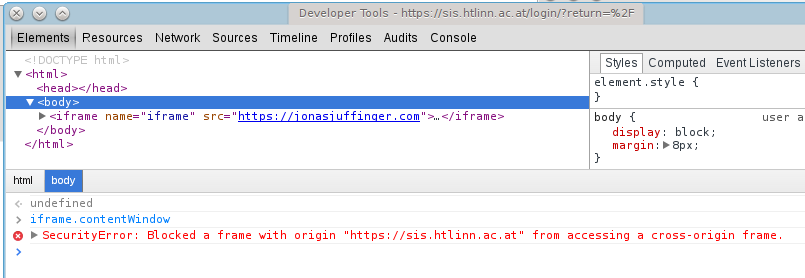
\includegraphics[keepaspectratio=true, width=14cm]{images/screenshots/xsrf0.png}
\caption{Browser blockiert Cross-Origin-Access auf iFrame}
\label{fig:content_security_xsrf0}
\end{figure}
\paragraph{Methoden um Vorzubeugen\\}
Es gibt einige Möglichkeiten, um diesem Problem vorzubeugen:
\begin{itemize}
	\item Die einfache Möglichkeit ist das Überprüfen des Referer-Feldes im HTTP-Kopf. Bei solchen XSRF-Angriffen wird üblicherweise das Referer-Feld auf die Seite des Angreifers umgeändert. Jedoch sollte man sich nicht auf dieses Feld verlassen, da viele Privatsphäre-Browser-Plugins  das Mitsenden dieses Feldes verhindern. Auch können Proxy-Server und ähnliches dieses Feld verändern.
	\item Über das HTTP-Feld \texttt{X-Frame-Options: SAMEORIGIN} wird der Webbrowser angewiesen, nur das Einbinden über Seiten mit dem gleichen Ursprung zu erlauben. Dieses Feld ist jedoch noch nicht bei allen Browsern implementiert, so sollte man sich nicht darauf verlassen.
	\item Die gängigste Variante, um dieses Sicherheitsproblem zu entfernen ist, eine zufällig generierte Zeichenkette an jedes Formular anzuhängen. Dieser Hash ist mit der PHP-Session verknüpft und authorisiert in gewisser Weise den Inhalt. In Fachkreisen wird oft von \enquote{Page-Token} oder von \enquote{Nonce} gesprochen. Der Angreifer hat - unter Annahme, der Webbrowser funktioniert ordnungsgemäß - keine Möglichkeit dieses Token auszulesen. Diese Möglichkeit wird auch bei SIS verwendet (siehe \gref{sec:content_draft_token}).
\end{itemize}
\subsubsection{Denial of Service (Klotz)}
\paragraph{Problem\\}
Als Denial of Service, bezeichnet man die Nichtverfügbarkeit eines Dienstes. Meistens spricht man von DoS wenn Service aufgrund einer Überlastung nicht mehr erreichbar ist. Die Nichtverfügbarkeit kann aber auch andere Gründe haben.\\
In unserem Fall stellt DoS keine allzu große Gefahr dar, da weder in Form von Rechenleistung noch in Form von Datenraten große Kapazitäten benötigt werden.\\

\paragraph{Methoden um Vorzubeugen\\}
Als Sicherheit wurde während des Testbetriebes des Systems der Traffic überprüft und überschlagsmäßig berechnet mit welchen Datenraten zu rechnen ist. Dabei haben wir festgestellt, dass wir mit unseren Datenraten weit unter der Grenze des an unserer Schule möglichen Traffics sind.\\
\subsubsection{Brute-Force Attack (Weiland)}
\paragraph{Problem}
Bei einer Brute-Force Attacke werden mangels fehlender Algorithmen solange mögliche Kombinationen ausprobiert, bis ein Erfolg, z.B. Zutritt zu mit Passwort gesichertem Bereich, eintritt.
\subparagraph{dictionary attack}
Bei einem Wörterbuchangriff werden zuerst häufig verwendete Passwörter wie zum Beispiel \enquote{password1!} oder \enquote{admin} ausprobiert. 
\subparagraph{reverse Brute-Force-Attack}
Hierbei wird ein Passwort mit verschiedenen Benutzernamen oder ein Schlüssel auf verschiedene verschlüsselte Daten angewendet, bis ein Vorgang erfolgreich ist.
\paragraph{Methoden um Vorzubeugen}
Eine zum teil sehr effektive Verhinderung von Brute-Force-Attacken kann dadurch erreicht werden, dass nur eine begrenzte Anzahl von Anmeldungsversuchen  zugelassen ist. Jedoch kann diese Sicherheitsvorkehrung auch umgangen werden. Wird die Anzahl der Anmeldungsversuche pro IP-Adresse gezählt, muss der Angreifer sich nur eine andere IP-Adresse geben, um weitere Versuche zu erhalten. Zudem ist diese Methode nutzlos, wenn der Angreifer die Attacke offline durchführt, wie zum Beispiel beim Versuch einen verschlüsselten Datenverkehr zwischen Client und Server zu entschlüsseln, da die Daten am Rechner des Angreifers liegen und weder der Server, noch der Client dies erkennen können. \\\\
Die am leichtesten anzuwendende Methode zum Verhindern bzw. Verlangsamen einer Brute-Force-Attacke ist ein möglichst langes Passwort mit Zahlen, Groß- und Kleinschreibung und Sonderzeichen. Hierfür gibt es mehrere Lösungsansätze, wie zum Beispiel ganze Sätze als Passwörter zu verwenden, da eine normale Brute-Force-Attacke nahezu unendlich lange benötigen würde. Jedoch ist zu beachten, dass für den Fall, dass der Angreifer das richtige Passwort gleich zu Beginn oder nach kurzer Zeit probiert, auch ein langes Passwort recht schnell geknackt ist, wobei die Wahrscheinlichkeit hierfür mit zunehmender Länge des Passworts sinkt.\\
\\
Mittels eines der im Internet angebotenen Passwortüberprüfer \\( \href{https://review.datenschutz.ch/passwortcheck/check.php}{https://review.datenschutz.ch/passwortcheck/check.php}) ergab zum Beispiel der Satz \enquote{Dieses\_Passwort\_ist\_sogar\_vor\_9\_Idioten\_sicher!} eine maximale Dauer von\\ 348'140'598'685'071'194'490'295'439'208'633'571'979'278'835'755'974'363'969'507'922'103'075 Jahre ($\approx 3,5 \cdot 10^{66}$ Jahre), wenn 2 Milliarden Versuche pro Sekunde durchgeführt werden. Nur zum Vergleich: Wissenschaftler sagen die Erde sei ca. 4,6 Milliarden Jahre alt. Das ist ca. um den Faktor 7.6 $\cdot 10^{58}$ weniger.


\newpage
\section{Lösungswege}

\subsection{PHP}
% Warum PHP? Welche Alternativen gäbe es?
\subsection{MySQL}
% Warum MySQL? Welche Alternativen gäbe es?
\subsection{Datenbankdesign}
Bei Design der Datenbank stellten sich einige grundlegenden Fragen:

\begin{itemize}
	\item Wie werden die Schulstunden gespeichert?
	\item Wie werden die Supplierungen gespeichert?
\end{itemize}

\subsubsection{Gewählte Lösung}
Die Gruppe entschied sich für folgende Lösung:\\
\\
Es gibt Tabellen für:\\
\begin{itemize}
	\item Abteilungen
	\item Klassen
	\item Fächer
	\item Lehrer
	\item Uhrzeiten
\end{itemize}
\vspace{0.03cm}
\begin{itemize}
	\item Die Basis-Stunden
	\item Die Stunden
\end{itemize}
\vspace{0.03cm}
\begin{itemize}
	\item fehlende Lehrer
	\item fehlende Klassen
\end{itemize}
\vspace{0.03cm}
\begin{itemize}
	\item Die Supplierung
\end{itemize}
Die Basis-Stunde verknüpft die Klasse der Stunde mit der Uhrzeit. Die Stunde verknüpft die Basis-Stunde mit dem Lehrer, dem Fach und dem Raum.\\
\\
Die Basis-Stunde wird benötigt, damit die Information, welche Klasse wann Unterricht hat, nicht mehrfach gespeichert werden muss.\\
\\
Die Tabellen für die fehlenden Lehrer und die fehlenden Klassen haben Spalten für eine Start- und End-Zeit.\\
\\
Die Supplierungs-Tabelle hat Felder für die Stunde, den Supplierlehrer, den neuen Klassenraum, die neue Start- und Endstunde, sowie Flags zum Ausblenden der Stunde auf dem angepassten Stundenplan.\\
Es ist möglich, mehrere Supplierungen für die gleiche Stunde einzutragen. Dieses Verhalten ist für manche Ausnahmefälle notwenig (siehe Beispiel).\\
\\
\begin{figure}[H]
\centering
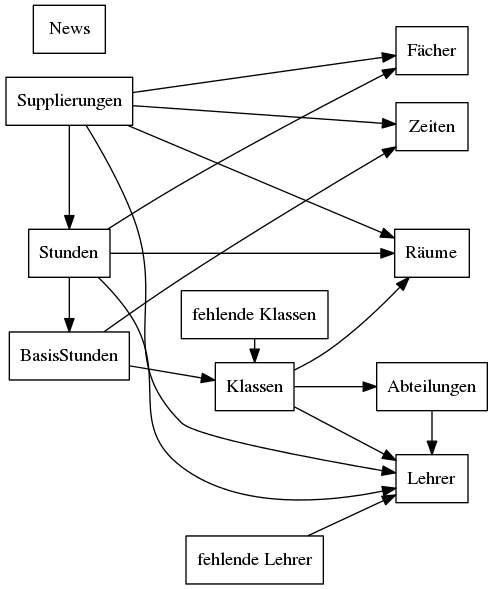
\includegraphics[keepaspectratio=true, width=10cm]{images/dbSubstitudes.png}
\caption{Supplierungs-Datenbank}
\end{figure}
Für das folgende Beispiel wird angenommen, dass eine Schulstunde 60 Minuten entspricht.\\
\\
\textit{Beispiel:} Klasse K hat am Montag um 8:00 eine Doppelstunde des Faches F mit Lehrer L in Raum R. Da der Lehrer zu spät kommen wird (ist bereits im vorhinein bekannt), soll nun die erste Stunde auf 16:00 in Raum P verschoben werden, die zweite Stunde soll aber bleiben.\\
\\
\textit{Lösung:} Die Doppel-Stunde wird 2 mal suppliert. Einmal mit dem selben Lehrer im selben Raum mit Start-Stunde um 9:00 und End-Stunde um 10:00. Und das zweitemal mit dem selben Lehrer im Raum P mit Start-Stunde um 16:00 und End-Stunde um 17:00.

\subsubsection{Alternative Lösungen}

Eine alternative Lösung, die angedacht wurde, ist folgende:\\
\\
Ansatt zwei Tabellen für die Basis-Stunde und die Stunde gibt es nur eine Stunden-Tabelle.
Diese verknüpft die Klasse mit der Uhrzeit, der Länge der Stunde, einem kombinierten Lehrer-Feld, einem kombinierten Fächer-Feld, einem kombinierten Raum-Feld.\\
\\
Die kombinierten Felden sollten den ersten Wert enthalten. Für jeden weiteren Wert wird der aktuelle Feld-Wert verodert mit dem nächsten Wert, welcher zuvor um ($x \cdot $(Anzahl der bisherigen Einträge)) Bits nach links verschoben wurde.\\
Hierbei wurde \textit{x} noch nicht bestimmt, es müsste so gewählt werden, dass der Eintrag mit der höchsten ID nicht in den dahinterliegenden Einträg überläuft (Für die Lehrer wäre $2^{8}$ (=256) ideal, da es knapp unter 200 Lehrer an der HTL gibt).\\
\\
Diese Lösungsmöglichkeit wurde allerdings verworfen, da es einiges an Aufwand ist, immer die richtigen Lehrer herauszulesen und da das Holen der Lehrer-Daten (Name, etc) nicht mehr im selben Query ausgeführt werden kann, als das Holen der Stundendaten, was bei mehr als 1 Zugriffspunkt zu Problemen mit der Daten-Konsistenz führen kann.
\subsection{HTTPS}

\subsubsection{Gewählte Lösung}

\subsubsection{Alternative Lösungen}
\subsection{Mobile App}

\subsubsection{Gewählte Lösung}

\paragraph*{Hybrid-App\\}

Die App wird als Hybrid-App realisiert, dabei handelt es sich um eine Applikation welche zwar mit Webtechnologien erstellt wird aber lokal auf dem Gerät betrieben wird.
Die mobile App wird aus Webseiten mit HTML, JavaScript und CSS aufgebaut. Diese Dateien werden dann mit Hilfe des Frameworks PhoneGap zu einer App für Android, WindowsPhone und iOS kompiliert. Zur Kommunikation mit dem Server sind noch einige PHP-Dateien auf dem Server gespeichert.


\subsubsection{Alternative Lösung}
\paragraph*{Native App\\}

Es könnte auch eine native App erstellt werden dann müsste aber für jedes der drei Betriebssysteme eine eigene App erstellt werden.\\
\\
Android:\\
Native Android-Apps werden grundsätzlich in Java programmiert. Um solche Applikationen zu erstellen wird aber gewisse Software benötigt.\\
Es muss eine Entwicklungsumgebung (IDE), zum Beispiel Eclipse, auf dem Rechner installiert werden und nachträglich müssen noch die Android Development Tools (ADT) installiert werden. Alternativ gibt es noch die Möglichkeit Android Studio von Google zu installieren, dabei handelt es sich um eine vollständige Android-Entwicklungsumgebung, mit einigen Extras wie zum Beispiel einem Layout-Editor.\\
\\
WindowsPhone:\\
WindowsPhone-Apps werden in C\# programmiert.\\
Zum erstellen einer WindowsPhone-App muss zuerst VisualStudio installiert werden. Damit können dann Apps für WindowsPhone entwickelt werden. In VisualStudio ist sogar ein Simulator integriert mit welchem es möglich ist die Apps zu testen bevor man sie auf ein Smartphone lädt.\\
\\
iOS:\\
Für die Entwicklung einer iOS-Apps benötigt man als erstes einen Mac(Apple-Computer), da es die Entwicklungssoftware für iOS-Apps(XCode) nur für Mac gibt.\\
Um eine iOS Applikation zu erstellen muss man zuerst die Entwicklungssoftware, XCode, herunterladen und installieren. Mit Hilfe dieser Software kann man nun erste Apps erstellen. Die grafische Oberfläche der App kann man noch sehr einfach durch Drag and Drop Funktionen erstellen. Um den Schaltflächen jedoch Funktionen zuzuweisen muss man auch wieder programmieren. Bei der verwendeten Programmiersprache handelt es sich um Objective-C, eine objektorientierte Programmiersprache mit Ähnlichkeiten zu C++ und C\#.
Die programmierten Applikationen kann man dann im integrierten Simulator testen.
Um die Applikationen auf echten Geräten zu testen benötigt man bereits eine Entwicklerlizenz, diese kostet 99\$ pro Jahr(Preis von https://developer.apple.com/programs/ios).\\
\\
Native Applikationen sind zwar wesentlich schneller als hybrid Apps, aber diese Lösung wurde nicht gewählt, da es viel zu aufwendig ist für jedes Betriebssystem eine eigene Entwicklungsumgebung zu installieren und die App drei mal in den jeweiligen Programmiersprachen zu programmieren und zu erstellen. Und da keiner der an der Diplomarbeit beteiligten Schüler ein PC von Apple besitzt wäre es uns nicht möglich gewesen eine iOS-App auf diesen Weg zu erstellen.\\

\paragraph*{Web-App\\}

Eine weitere Alternative ist die Entwicklung einer Webapp.\\
Bei einer Webapp handelt es sich prinzipiell um eine Webseite, welche für Smartphones optimiert wurde, beim Öffnen der Applikation wird einfach die gewünschte Webseite geladen.\\
Die Entwicklung einer Webapp würde sich kaum von der Entwicklung einer hybrid App unterscheiden, aber bei der Webapp hat man den Vorteil, dass auch PHP-Seiten verwendet werden können. Dadurch ist die Übertragung der Daten und die Authentifizierung wesentlich einfacher.\\
Eine Webapp hat aber den Nachteil, dass sie langsamer ist als eine Applikation welche lokal auf dem Gerät installiert ist und ein weiterer Nachteil für den Nutzer ist, dass bei dieser Lösung ein wesentlich größerer Bedarf an Internetdatenvolumen anfällt.\\

% warum phonegap, was wären die alternativen gewesen? vor-, nachteile?
\subsection{Verbindung App $ \leftrightarrow $ Server}
% Wie funktioniert die Verbindung zwischen App und Server?

Bei der Verbindung zwischen dem Server und der App muss darauf geachtet werden, dass die App zwar als Website entwickelt wurde aber lokal ausgeführt wird. Darum können die Daten nicht einfach mit PHP aus der Datenbank geladen und direkt weiterverarbeitet werden.\\

\subsubsection{Gewählte Lösung}
Die Lösung hierfür war, dass über das Source-Attribut eines Script-Tags eine PHP-Datei am Server eingebunden wurde, welche die Daten aus der Datenbank lädt. Diese Daten werden dann in Form eines JSON-Objektes gespeichert. Mit Hilfe des ECHO-Befehls wird die Objektdeklaration und das Zuweisen der Daten in die Datei geschrieben. Dadurch kann dieser Code als JavaScript ausgeführt werden wenn er auf dem Gerät geladen wird. Weiters steht in dieser Datei noch der JavaScript-Code welcher die Daten verarbeitet.\\
Dadurch, dass bei dieser Art des Datenaustausches auch noch der JavaScript-Code zum verarbeiten der Daten mitgeladen wird, hat man den Vorteil, dass viele Teile der App durch diesen JavaScript-Code und somit ohne Update der App verändert werden können.\\

\subsubsection{Alternative Lösungen}
Eine andere Möglichkeit wäre die JSON-Callback Funktion. Dabei ist auf dem Server ein PHP-File in welchem die benötigten Daten mittels MySQL aus der Datenbank abgerufen und als JSON gespeichert werden. 
Mit Hilfe der Funktion getJSON(), kann nun auf der lokalen Webseite durch Angabe der URL der PHP-Datei die Daten auf die lokale Seite geladen werden.\\
Ein Problem bei dieser Verbindungsvariante ist, dass es nur schwer machbar ist, nach dem Laden der Daten erneut einen JavaScript-Code auszuführen, welcher dann die Daten verarbeitet, da im Normalfall der gesamte Code sofort beim Aufruf der Webseite ausgeführt wird.\\

% Alternative Lösungen?
% Vor-, Nachteile?
%
% Teilweise kannst du das, das du bei den Technologien (Phonegap) geschrieben hast, hierher verschieden.

\subsection{PDF-Generierung}
Die PDF-Generierung wird mittels FPDF durchgeführt.\\
\\
Der Vorteil in dieser Variante gegenüber anderen PDF-Lösungen liegt darin, dass auf dem Server nichts installiert werden muss. Es muss nur das Archiv, welches auf der Website von FPDF (\href{www.fpdf.org}{www.fpdf.org}) downloadbar ist, auf dem Server entpackt werden. Von diesem Verzeichniss werden jedoch nur die Datei \enquote{fpdf.php} und der Ordner mit den Font-Styles benötigt. Die restlichen Dateien wurden gelöscht.\\
Zudem bietet eine Lösung mittels generiertem PDF auch den Vorteil, dass der Ausdruck ohne großen Aufwand auf einem Rechner gespeichert werden kann.
\\
Ein Nachteil der Verwendung von FPDF ist jedoch, dass das Design aufgrund der Zellenstruktur nur schwer zu Ändern bzw. Erstellen ist. Besonders die Kopf und Fußzeile sind nicht leicht zu verändern.\\\\
Eine andere Möglichkeit eine Druckausgabe zu erzeugen, wäre, wie im Vorgängerprojekt verwendet wurde, eine ausdruckbare Website. In diesem Fall wäre der Ausdruck jedoch nicht sofort als PDF erstellt worden und hätte um ein PDF zu erstellen mit einem PDF-Drucker ausgedruckt werden müssen. Allerdings ließe sich das Design leichter ändern.


\subsection{Prinzip des Monitor-Systems}

Als Thin-Client für die Monitore werden Raspberry Pis verwendet.\\
Die Kommunikation zum Server und die Art des Anzeigens der abgerufenen Informationen wird mithilfe eines Webbrowsers gelöst. Es wurde der Webbrowser Chromium ausgewählt, da dieser die neuesten HTML5 Standards implementiert hat und auf den Raspberry Pis laufen kann.

\subsubsection{Laden der Daten}

Für das Laden der Daten vom Webserver wird Javascript in Verbindung mit AJAX verwendet.\\
Dies hat gegenüber dem Neuladen der Seiten den Vorteil, dass, im Falle dessen, dass der Webserver kurzzeitig nicht erreichbar ist, das System trotzdem ohne Probleme weiter laufen kann - sieht man davon ab, dass mit der zeit, die angezeigten Daten veralten.\\
Der einzige Zeitpunkt, an dem der Server auf alle Fälle erreichbar sein muss, ist der Start der Raspberry Pis, da hier die Website vom Server geladen werden wird. Auch diese Bedingung hätte entfernt werden können, indem man die Seite lokal abgelegt hätte. Dies hat allerdings den Nachteil, dass die Seite über ein weiteres Script hätte immer auf dem aktuellen Stand gebracht werden.

\subsection{Authentifizierung der Monitore}

Es stellt sich die Frage, die die Monitore am Server registriert werden. Da alle Monitore über das Webinterface zentral administriert werden können, ist es äußerst kontraproduktiv, wenn eventuell Schüler - oder gar Außenstehende - die Datenbank-Tabelle für die registrierten Monitore fluten können.\\
\\
Es wurde von den Betreuern vorgegeben, dass für sämtliche Verbindungen zum Server HTTPS verwendet werden sollte (siehe Lösungswege/HTTPS). Dies führt bei der Registrierung der Monitore zu Problemen (siehe folgendes).

\subsubsection{Gewählte Lösung}

Da zu anfangs nicht klar war, welches IP-Netz das W-LAN der Monitore bekommen sollte, konnte keine IP-Filterung verwendet werden.\\
\\
Das Problem wurde gelöst, indem in der Datenbank für die Monitore eine Spalte für die IP-Adresse vorgesehen wurde. Die Idee bestand darin, dass jede IP-Adresse nur maximal einen Monitor registrieren darf (Vgl. \autoref{sec:content_solutions_monitors_alt_reg}).\\
\\
Aufgrund dessen, dass für die verschlüsselte Verbindung die Packete nach außen geNATet werden und wieder durch die Firewall zurück kommen, haben alle Monitore die öffentliche IP-Adresse der Schule.\\
Um dieses Problem zu umgehen wurde mit Betreuer Lassnig vereinbart, dass die Verbindung der Monitore unverschlüsselt sein darf, da keine sicherheitsrelavanten Daten übertragen werden, und da das W-LAN selbst schon verschlüsselt.\\
Als Ziel-Adresse wird also anstatt https://sis.htlinn.ac.at http://sis.clients.htlinn.ac.at eingetragen.


\subsubsection{Alternative Lösungen}

\paragraph{Registrierung}
\label{sec:content_solutions_monitors_alt_reg}

Die Registrierung der Monitor hätte manuell erfolgen können. Hier würden mehrere Möglichkeiten in Frage kommen:

\begin{description}[style=nextline]
	\item[Registrierung nur vom Administrator-Interface aus]
		Dies hat den Nachteil, dass es zu frustrierenden Situationen kommen kann, wenn der tatsächliche Name des Monitors (eingestellt im Raspberry Pi) mit dem in der Datenbank nicht identisch ist.\\
	\item[Registrierung mittels Passwort]
		Ein Nachteil dieser Variante ist, dass das Passwort direkt an den Raspberry Pis eingegeben werden muss. Was den administrativen Aufwand vergrößert.
		Weiters muss dieses Passwort für Konfiguration mehr oder weniger öffentlich zugänglich sein muss, was den Zusatzaufwand nichtig macht.
	\item[Registrierung mittels Cookie-Hash]
		Diese Variante hat ähnliche Nachteile, wie die Registrierung mittels Passwort.
\end{description}

\paragraph{Verschlüsslung}

Als Alternative zur fehlenden Verschlüsslung hätte ein, von der HTL ausgestelltes SSL-Zertifikat für die Wild-Card-Domain *.clients.htlinn.ac.at ausgestellt werden können, den Raspberry Pis hätte man dann müssen das HTL-Root-Zertifikat importieren müssen. Dies ist allerdings mit recht viel administrativen Aufwand verbunden, daher wurde diese Idee verworfen.\\
Als eine weitere Variante hätte man den Raspberry Pis den Server, auf dem die Website abgelegt wurde, als SSL-Ausnahme eintragen können. 
\subsection{Benutzermanagement}
In der Schule sind im Wesentlichen 4 Berechtigungsstufen vorhanden.
\begin{itemize}
	\item Schüler
	\item Lehrer
	\item Abteilungs-Vorstände
	\item Administratoren
\end{itemize}
Diese Gliederung wird 1:1 in SIS übertragen, allerdings wird zusätzlich eine Gruppe für die \enquote{Newsbeauftragten}, welche gegenüber den Schülern/Lehrern zusätzlich die Berechtigung haben, den Abteilungsvorständen News vorzuschlagen, vorgesehen.\\
Da die Benutzer-Authentifizierung über den LDAP-Server läuft, liegt der Gedanke nahe, dass auch die Autorisierung über LDAP laufen könnte.\\
Da alle Lehrer automatisch im eDirectory-Container ou=LEHRER,o=HTLinn und die Schüler automatisch im eDirectory-Container ou=STUDENTS,o=HTLinn liegen, lässt sich anhand des DN des Benutzers ausgelesen werden, ob es sich um einen Lehrer oder um einen Schüler handelt.\\
\subsubsection{eDirectory-Gruppen}
Für alle weiteren logischen Gruppen werden vom eDirectory-Administrator auch dementsprechende eDirectory-Gruppen erstellt:
\begin{itemize}
	\item cn=SIS-SuperUser,ou=SIS,o=HTL1
	\item cn=SIS-News,ou=SIS,o=HTL1
	\item cn=SIS-Admin-E,ou=SIS,o=HTL1
	\item cn=SIS-Admin-M,ou=SIS,o=HTL1
	\item cn=SIS-Admin-N,ou=SIS,o=HTL1
	\item cn=SIS-Admin-W,ou=SIS,o=HTL1
\end{itemize}
Es ist prinzipiell möglich, dass ein Benutzer Mitglied mehrerer eDirectory-Gruppen ist.\\
\subsubsection{Verwendung}
Meldet sich ein Benutzer an, so werden seine Berechtigungen (sprich Gruppen-Zugehörigkeiten) am LDAP-Server abgefragt und in der PHP-Session gespeichert. Auch, ob es sich um einen Lehrer handelt, wird in der Session gespeichert. Dies hat den Vorteil, dass nur einmal die Berechtigungen abgefragt werden müssen.\\
Jedes PHP-Script kann die Berechtigungen über die PHP-Session abfragen und mehr oder weniger autonom entscheiden, welche Berechtigungen der Benutzer erhält.
\subsection{Wurzelverzeichnis}
\label{sec:content_solutions_root}
Das Projekt soll auch funktionsfähig sein, wenn es nicht dem Grundverzeichnis des virtuellen Hosts liegt. Das ist prinzipiell kein Problem, da alle Dateien relativ zum eigenen Standort referenziert werden können. Allerdings gibt es eine \enquote{Hauptdatei} (/modules/general/Main.php), die von allen Seiten inkludiert wird, da sie grundlegende Funktionen zur Verfügung stellt. Diese Datei inkludiert ihrerseits wiederum weitere Dateien, welche beispielsweise das Management der Sessions übernehmen. Werden diese Dateien relativ von der Hauptdatei  inkludiert, so werden sie in Wirklichkeit von der eigenen Datei inkludiert, da der Quellcode eingefügt wird. Das hat zur Folge, dass die referenzierten Dateien nicht existieren.\\
Dieses Problem wurde gelöst indem eine \enquote{Konfigurations}-Datei erstellt wird, in der der relative Pfad zum Projekt-Root-Verzeichnis vom Document-Root des Webservers, sowie der absolute Pfad des Root-Verzeichnises im Dateisystem definiert werden. Diese Datei wird von allen weiteren Dateien inkludiert, die weitere Einbindung von Dateien erfolgt nun nicht mehr über den relativen Pfad von der eigenen Position aus, sondern über die Root-Definition in der \enquote{Konfigurations}-Datei.

\newpage
\section{Entwurf} % Grobentwurf

\subsection{Dateibaum}
\label{sec:files}
Der Aufbau der Ordnerstruktur für das Projekt wird folgendermaßen festgelegt.

\begin{description}[style=nextline]
	\item[/backend/]
		Hier befindet sich das Menü für die Eingaben.\\
		Dieses Menü ist für die Benutzergruppen \enquote{SIS-Admin-E}, \enquote{SIS-Admin-N}, \enquote{SIS-Admin-M}, \enquote{SIS-Admin-W}, \enquote{SIS-News} und \enquote{SIS-SuperUser} verfügbar.
		\begin{description}[style=nextline]
			\item[./absentees/]
				Hier befindet sich das Menü für das Eintragen der Fehlenden.\\
				Dieses Menü ist für die Benutzergruppen \enquote{SIS-Admin-E}, \enquote{SIS-Admin-N}, \enquote{SIS-Admin-M}, \enquote{SIS-Admin-W} und \enquote{SIS-SuperUser} verfügbar.
				\begin{description}[style=nextline]
					\item[./classes/]
						Hier können fehlende Klassen eingetragen werden.\\
						Dieses Formular ist für die  Benutzergruppen \enquote{SIS-Admin-E}, \enquote{SIS-Admin-N}, \enquote{SIS-Admin-M}, \enquote{SIS-Admin-W} und \enquote{SIS-SuperUser} verfügbar.
					\item[./teachers/]
						Hier können fehlende Lehrer eingetragen werden.\\
						Dieses Formular ist für die  Benutzergruppen \enquote{SIS-Admin-E}, \enquote{SIS-Admin-N}, \enquote{SIS-Admin-M}, \enquote{SIS-Admin-W} und \enquote{SIS-SuperUser} verfügbar.
				\end{description}
				\item[./administration/]
					Hier befindet sich das Administratoren-Menü.\\
					Dieses Menü, sowie alle Unterpunkte, sind nur für die Benutzergruppe \enquote{SIS-SuperUser} verfügbar.
					\begin{description}[style=nextline]
						\item[./classes/]
							In diesem Formular können die Klassen modifiziert werden.
						\item[./hours/]
							Hier können die zeitlichen Unterrichtsstunden verändert werden.
						\item[./lessons/]
							In diesem Formular können die Stundenpläne verändert werden.
						\item[./rooms/]
							Hier können die Räume eingetragen werden.
						\item[./sections/]
							Hier können die Abteilungen modifiziert werden.
						\item[./subjects/]
							Fächer können hier hinzugefügt werden.
						\item[./teachers/]
							In diesem Formular können die Lehrer modifiziert werden.
					\end{description}
				\item[./monitors/]
					Alle Einstellungen für die Monitore sind hier zu finden.\\
					Dieses Formular ist für die Benutzergruppen \enquote{SIS-Admin-E}, \enquote{SIS-Admin-N}, \enquote{SIS-Admin-M}, \enquote{SIS-Admin-W} und \enquote{SIS-SuperUser} verfügbar.
				\item[./news/]
					In diesem Punkt können News eingetragen werden.\\
					Dieses Menü ist für die Benutzergruppen \enquote{SIS-Admin-E}, \enquote{SIS-Admin-N}, \enquote{SIS-Admin-M}, \enquote{SIS-Admin-W}, \enquote{SIS-News} und \enquote{SIS-SuperUser} verfügbar.
				\item[./substitudes/]
					Hier befindet sich das Menü für die Auswahl der Abteilung bei den Supplierungen.\\
					Dieses Menü ist nur für die Benutzergruppe \enquote{SIS-SuperUser} verfügbar.
					\begin{description}[style=nextline]
						\item[./form/]
							Hier können die Supplierungen eingetragen werden.\\
							Dieses Formular ist nur für die Benutzergrupppen \enquote{SIS-Admin-E}, \enquote{SIS-Admin-N}, \enquote{SIS-Admin-M}, \enquote{SIS-Admin-W} und \enquote{SIS-SuperUser} verfügbar.
					\end{description}
		\end{description}	
	\item[/cookies/]
			Hier müssen vor dem Betreten der Seite die Cookies akzeptiert werden.
		\item[/data/]
			\begin{description}[style=nextline]
				\item[./fonts/]
					Alle Schriftart-Dateien liegen hier.
				\item[./images/]
					Hier befinden sich sämtliche Bilder.\\
					Dateien, welche sich logisch gruppieren lassen, besitzen eigene Ordner.
				\item[./scripts/]
					Alle Javascripts, welche in Dateien extrahiert wurden, sind hier zu finden.
				\item[./styles/]
					Hier sind sämtliche Stylesheets.	
			\end{description}
		\item[/impressum/]
			Wie der Name schon sagt, ist hier das Impressum zu finden.
		\item[/login/]
			Hier befindet sich der Login.
		\item[/logout/]
			Und hier ist der Logout.
		\item[/logs/]
			Hier sind spezielle Log-Dateien zu finden.
		\item[/mobile/]
			Die Mobil-Seite befindet sich hier.
			\begin{description}[style=nextline]
				\item[./api/]
					Hier ist die API für die App hinterlegt.
			\end{description}
		\item[/modules/]
			Hier sind die verschiedenen Module des Systems bzw. ihre Komponenten  gespeichert.
			\begin{description}[style=nextline]
				\item[./datebase/]
					Dateien für den allgemeinen Zugriff auf die Datenbank werden hier gespeichert.
				\item[./design/]
					Die HTML-Dateien der Designs werden hier abgelegt.
				\item[./external/]
					Fremdmodule werden hierher kopiert.
				\item[./form/]
					Hier finden sich Dateien mit Funktionen für den Aufbau von HTML-Formularen.
				\item[./general/]
					Allgemeine, wichtige Module sind hier untergebracht. U.a. findet man hier die Dateien für den Zugriff auf die Datenbank, das Session-Management oder den Zugriff auf LDAP.
				\item[./menu/]
					Die Dateien in diesem Ordner dienen zum Generieren der Haupt-Menüstruktur.
				\item[./monitors/]
					Dateien, die das Monitorsystem betreffen, sind hier zu finden.
				\item[./other/]
					Alle Module, die sich nicht einordnen lassen, werden hier untergebracht.
			\end{description}
		\item[/monitors/]
			Hier ist der Startpunkt für das Monitorsystem.
			\begin{description}[style=nextline]
				\item[./api/]
					Hier befindet sich die API für die Monitore.
				\item[./media/]
					Inhaltbezogene Mediendateien (Bilder und Videos) für das Monitorsystem werden hier gespeichert.
			\end{description}
		\item[/news/]
			Die Website für die News liegt hier.
		\item[/pdf/]
			Hier werden die Druckversionen als PDF zur Verfügung gestellt.
		\item[/substitudes/]
			Die Supplierpläne werden hier generiert.
		\item[/timetables/]
			Der eigene Stundenplan wird hier generiert.
			\begin{description}
				\item[./all/]
					Lehrer können hier die Klassenstundenpläne ansehen.
			\end{description}
		\item[/tmp/]
			Ordner für temporäre Dateien.
\end{description}

Zusätzlich gibt es im Projekt ein Verzeichnis /raspberryConfig/. Hier werden Konfigurationsdateien für die Raspberry Pis hinterlegt.
\subsection{Datenbankdesign}

Das Konzept des Datenbankdesigns wird bereits unter \gref{sec:content_solution_db} behandelt.

Hinzu kommt noch das das Monitorsystem.

\subsubsection{Monitorsystem}

Damit die Monitore einen Supplierplan anzeigen können, muss jeder Monitor einer Abteilung zugeordnet sein.\\
Auch müssen die Monitore, damit sie die Raumstundenpläne anzeigen können, mit einem Raum verknüpft sein.\\
\\
Zusätzlich dazu sollen die Monitore (beziehungsweise die dahinterliegenden ThinClients) wissen, was sie anzeigen sollen (Stundenplan, Supplierplan, Bilder, etc). Hierzu wird eine Tabelle für den Typ des Monitors erstellt und diese verknüpft.\\
\\ 
Für die Erweiterung des Monitorsystem um das Display-Steuer-System muss eine weitere Tabelle für die Display-Typ (permanent ein, permanent aus, automatisch) vorgesehen und verknüpft werden (für Details, siehe \gref{sec:report}).\\
\\
Es ergibt sich folgendes Datenbank-Layout für die Monitore:
\begin{figure}[H]
\centering
\fdot[]{images/dbMonitors}{}
\caption{Supplierungs-Datenbank}
\end{figure}

\subsection{Monitorsystem}

\subsubsection{Grundsätzlicher Seiten-Aufbau}

Der Aufbau der, auf den Monitoren angezeigten, Seite wird folgendermaßen festgelegt.\\
Rechts unten wird Platz für eine Uhrzeit- und Datumsanzeige vorgesehen. Links daneben werden später die raumspezifischen Beschriftungen angezeigt.\\
Rechts oben soll der aktive Modus des Monitors am Hintergrund angezeigt werden. Horizontal und vertikal zentriert wird im Hintergrund das SIS-Logo platziert.\\
Der Platz oberhalb der Uhr steht Inhalten zur Verfügung, auch wenn dieser das SIS-Logo oder den Text rechts oben verdecken sollte.

\subsubsection{Initialisierung}

Wird die Seite geöffnet, so wird die Seite grundsätzliche aufgebaut.\\
Nun werden zwei Timer gestartet, von denen einer die Uhr aktualisiert (jede Sekunde) und der andere den Inhalt aktualisiert (10 Sekunden).

\subsubsection{Verringerung des Traffics}
Damit der Durchschnittliche Traffic möglichst gering gehalten werden kann, wird beim Anfragen des Inhalts am Server ein Hash generiert, welcher eindeutig den aktuellen Inhalt identifiziert. Dieser Hash wird mitgesendet und am Client gespeichert. Nun wird mit jeder weiteren Anfrage der Hash des Clients mitgesendet, sollten der Client-Hash und der neu generierte Hash am Server übereinstimmen, so wird ein Flag gesendet, dass sich der Inhalt nicht geändert habe. Der eigentliche Inhalt aber wird nicht gesendet.\\
Da sich die Inhalte relativ zum Aktualisierungszyklus des Clients sehr selten ändern, kann der Traffic so um weit über 50 \% reduziert werden.

\subsubsection{Multi-Modi}
Für den Monitor-Modus \enquote{Supplierplan \& News} wird am Server ein Sonderfall vorgesehen.\\
Es wird eine zusätzliche Variable mit gesendet, diese identifiziert den \enquote{Submode}, also quasi ob Supplierplan oder die News gesendet werden sollen. Wann sich der Submode ändert wird durch eine weitere Variable vorgegeben. Diese enthält den Timestamp der nächsten Änderung. Diese beiden Variablen werden vom Server generiert und vom Client zwar gespeichert, aber nicht mehr verändert, bis der Server neue Werte mitgibt.
\subsection{Design (Machac)}
\label{sec:content_design}
Das Folgende wurde von Philipp Machac geschreiben. Er war als eine Art externer Mitarbeiter für das Design der Seite verantwortlich. Die Implementierung wurde allerdings vom SIS-Team durchgeführt.
\subsubsection{Enstehung}
Die grundsätzliche Idee ist es, ein Design zu schaffen, welches im Gegensatz zu den meisten anderen Dingen unserer Anstalt, einladend und angenehm zu betrachten ist. Dementsprechend wurde ein unauffälliger Hintergrund mit warmen Farben gewählt, in diesem Fall Brauntöne. Als angenehm empfand ein Großteil der befragten Personen einen Holzhintergrund, von Verfechtern oftmals nur „Wohnzimmerboden“ genannt.\\
Da zum Zeitpunkt des Entwurfes gerade eine hitzige Diskussion bezüglich des Namens im Gange war (HTL Peter Anich, HTLinn oder einfach HTL Anichstraße) wurde das Design daraufhin ausgelegt, egal wie diese Diskussion auch enden sollte, autonom und für jegliche Änderungen gerüstet zu sein.\\
Das Logo der HTL mag ein toller Einfall gewesen sein, bezogen auf die Form und die Umsetzung der 4 Abteilungsfarben im Logo, zur Einpflegung in ein Design stellt es allerdings aufgrund der vielen unterschiedlichen Farben eine mittlere Katastrophe dar. Deswegen wurde entschieden das Logo einfarbig (Schwarz mit Transparenz) mit durchsichtigen Konturrändern, zur besseren Unterscheidung der Flächen innerhalb des Logos, umzubauen. Durch diesen Effekt wirkt das Logo fast wie \enquote{auf dem Holz eingebrannt}.\\
\enquote{Simplicity} ist eine weitere Eigenschaft, die das Design auszeichnen sollte, weshalb das gesamte Layout darauf ausgelegt ist, mit zwei, maximal aber 3 Farben auszukommen. Zulässige Schriftfarben sind nur Schwarz (ggf. mit Transparenz) und Weiß, sämtliche Grafiken sind Schwarz mit einer Opacity (Transparenz) und nur Transparent (also Hintergrund kommt durch).\\
Da zu  einem schlichten Design auch die verwendete Schriftart eine beträchtliche Rolle spielt, wurde von uns, die unserer Ansicht nach sehr schlichte Font \enquote{Century Gothic} verwendet. Diese zieht sich ebenfalls durch das ganze System, vom Webinterface über die App bis zu den Monitoren. Lediglich für den Text im Banner wurde ein auffälligerer, etwas freakig wirkender Schriftzug verwendet (Abduction2002), welcher dem Benutzer mitteilt, wo er sich befindet bzw. was er gerade sieht, z.B. SIS.Web Access oder auf den Monitoren z.B. SIS.Supplierungen oder SIS.News.\\
Diese Elemente (Header, Hintergrund und Logo) ziehen sich sowohl im Webinterface als auch auf den Monitoren wie ein roter Faden durch das System.\\
\subsubsection{Webinterface}
\label{sec:content_draft_design_web}
Das Webinterface sollte einen \enquote{WOW – Das ist aber cool}-Effekt erzeugen. Die einzelnen Menüpunkte sollten logisch angeordnet sein und sich gut in das Gesamtbild mit modifiziertem HTL Bild und Hintergrund einbinden. Deshalb wurde die Idee geboren, das Logo in der Mitte als zentralen Ausgangspunkt für die Menüführung zu verwenden. Die Buttons wachsen als Parallelogramme aus den vier Flächen des Logos, jeweils maximal zwei. Wird also die Maximalanzahl von acht Buttons erreicht, wirkt das Gesamtpaket einem Raumschiff ähnlich.\\
Um die Menüführung für den Benutzer sinnvoll und übersichtlich zu gestalten und trotzdem die Maximalanzahl an Buttons pro Seite nicht zu überschreiten, wurde die Menüführung in drei Teile aufgeteilt.\\
Die erste Seite stellt Informationen für den User da, unabhängig davon, ob dieser selbst noch administrative Funktionen erfüllt oder nicht. Es werden seine persönlichen Supplierungen, sein persönlicher Stundenplan und die Newsansicht zur Verfügung gestellt. Der Button rechts unten stellt jeweils den Schritt zum nächsten Menü dar. Auf der zweiten Seite finden sich administrative Möglichkeiten wieder, welche für den täglichen Gebrauch nötig sind. Hier sind also Punkte zur Eingabe der Supplierpläne und der fehlenden Lehrer, der News und das Management der Monitore. Auffällig ist hier, dass der Versuch unternommen wurde, zusammengehörige Punkte auch so anzuordnen (Menüübergreifend). So findet sich rechts oben auf der ersten Seite (SIS.Web Access) die Anzeige der Supplierungen, auf der zweiten Seite (SIS.Inputs) die Eingabe der fehlenden Lehrer und der Supplierungen wieder. Ebenso links unten die News zur Anzeige auf der ersten, die Eingabe selbiger auf der zweiten Seite. Somit ist das Menü etwas intuitiver gestaltet, als wenn die Anordnung anders wäre.\\
Da die zahlreichen Administrationsmöglichkeiten eine Seite mit acht Buttons sprengen würde, wurden eher selten genutzte Funktionen wie das Ändern der Stunden oder die Eingabe neuer Lehrer oder Stundenpläne auf ein drittes Menü ausgelagert (SIS.Administration), welches wiederum über den Button rechts unten erreicht werden kann.\\
\begin{figure}[H]
\centering
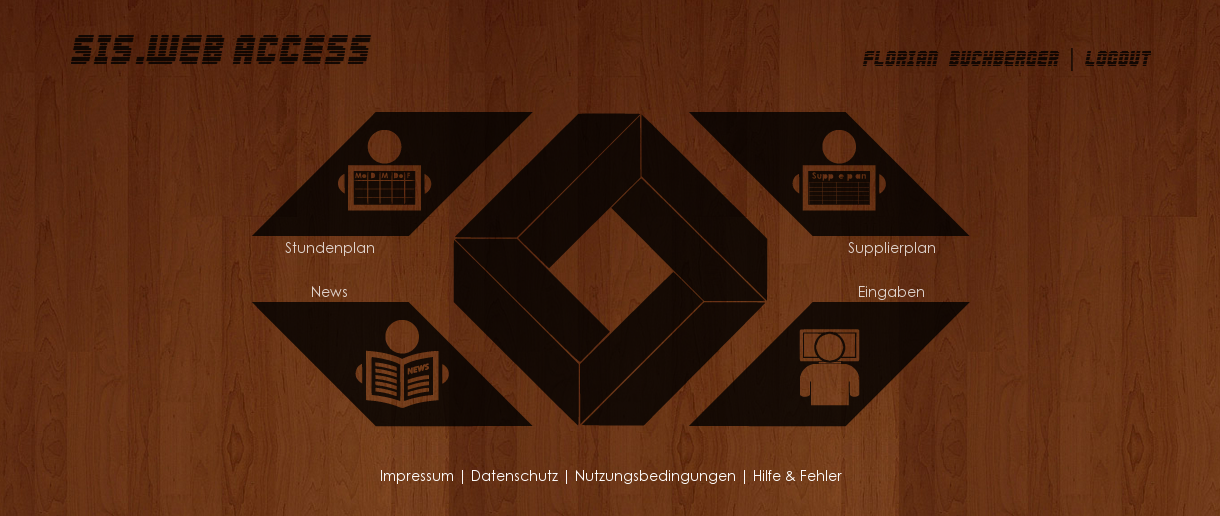
\includegraphics[keepaspectratio=true, width=14cm]{images/screenshots/web-access_nohover.png}
\caption{SIS.Web Access}
\label{fig:content_draft_design_webaccess}
\end{figure}
\begin{figure}[H]
\centering
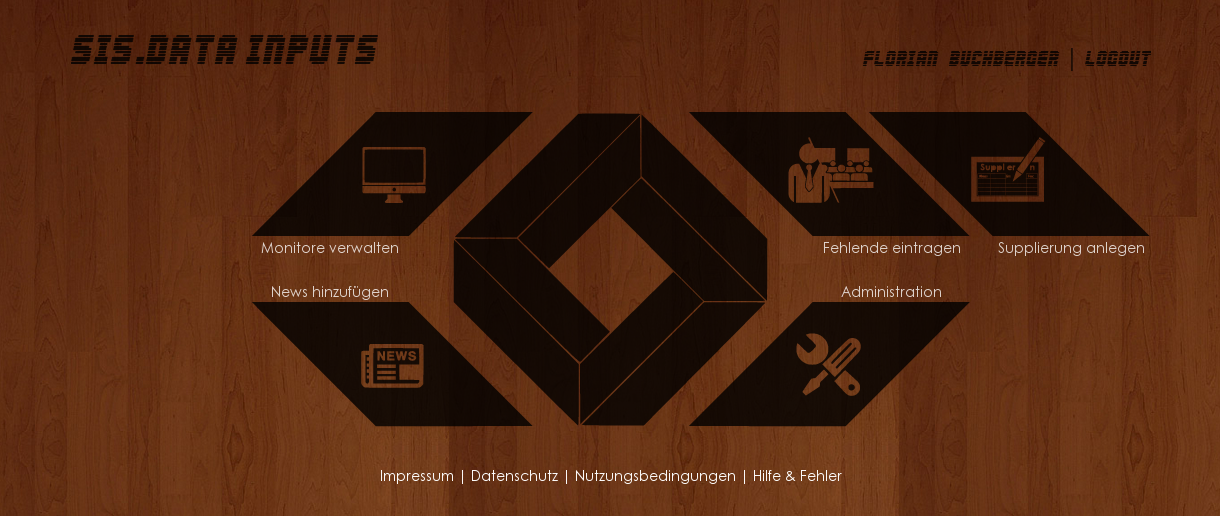
\includegraphics[keepaspectratio=true, width=14cm]{images/screenshots/data-inputs_nohover.png}
\caption{SIS.Data Inputs}
\label{fig:content_draft_design_datainputs}
\end{figure}
\begin{figure}[H]
\centering
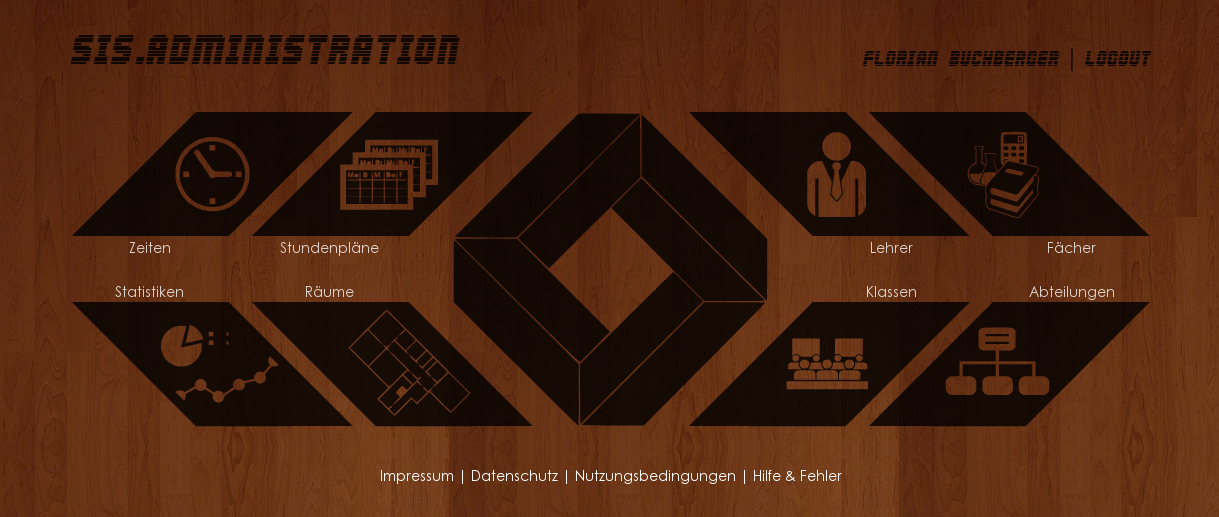
\includegraphics[keepaspectratio=true, width=14cm]{images/screenshots/administration_nohover.png}
\caption{SIS.Administration}
\label{fig:content_draft_design_administration}
\end{figure}
Mit Klick auf das Logo in der Mitte gelangt man jeweils zum vorhergehenden Menü zurück.\\
Die Buttons enthalten jeweils eine Grafik, welche den Punkt für den dieser Button steht, bestmöglich repräsentieren sollte. Ein Hoover Effekt bewirkt eine Änderung der Buttonfarbe (Schwarz auf Weiß) und weist den User daraufhin, welchen Button er aktuell gewählt hat. Dieser Effekt benötigt allerdings SVG Grafiken anstatt Beispielsweise png's, was die ganze Sache etwas kompliziert macht, dafür jedoch auch weniger Traffic – svg Grafiken sind kleiner – verursacht.\\
Da der Inhalt, welchen man erreichen soll nachdem ein Button geklickt wurde, seine Zusammengehörigkeit mit der eigentlichen Navigation/Menü nicht verlieren sollte wurde beschlossen, dass der neue Inhalt im Zuge einer Animation erscheint. Wird also ein Button angeklickt, wird der Monitor optisch quasi horizontal geteilt und auseinander geschoben. Im sich nun öffnenden Teil des Bildschirmes erscheint nun ein leicht dunklerer Hintergrund (ebenfalls Brauntöne), auf dem sich nach Beenden der Animation der Inhalt aufbaut. Um den Übergang zwischen den beiden Hintergründen sanfter zu gestalten, wurde eine weiße Linie dazwischen gezogen. Will man wieder in das Menü, kann nun entweder außerhalb des dunklen Hintergrundes auf den Bildschirm geklickt werden oder der Exit Button verwendet werden. Die Animation wird daraufhin entgegengesetzt ausgeführt und man ist wieder im ursprünglichen Menü.\\
All diese Features sind allerdings nur dann möglich, wenn Javascript aktiviert ist. Sollte das am Client PC nicht der Fall sein, wird eine Javascript-freie Seite geladen, ohne Animationen im Menü und lediglich mit der Möglichkeit, durch Anklicken des zugehörigen Buttontextes, den betreffenden Inhalt zu laden. Dieser erscheint in einem Vollbild und kann nur mit dem Exit Button wieder verlassen werden. Auf mobilen Geräten (iPhone, Android Devices usw.) wird zudem NUR die Seite ohne JS geladen, auch wenn das Device JS unterstützen würde.
\subsubsection{Monitordesign}
Die wichtigsten Inhalte, welche am Monitor angezeigt werden sind News, Supplierungen und Raumpläne. Die News werden mit weißer Schriftart in einem Schwarz transparenten Fenster mit abgerundeten Ecken angezeigt. Die Supplierungen in einer Tabelle, welche wiederum weiße Schrift auf schwarz transparentem Hintergrund ist, wobei die erste Zeile inverse Farben verwendet. Besonderheiten bei dieser Tabelle ist die Sortierung, welche nach Klassen erfolgt (vereinfacht das Lesen für die Schüler) sowie der Verzicht auf Vertikale Spaltenabtrennungen. Dies ermöglicht ein angenehmeres Lesen der Supplierungen. Die Raumbelegungspläne haben dieselbe Farbabstimmung wie der Supplierplan. Jede Zelle zeigt die drei Inhalte Klasse, Lehrer und Fach an, wobei die Klasse größer in der ersten Zeile und das Fach mit dem Lehrer in der nächsten Zeile in kleinerer Schriftart abgebildet sind.
\subsection{Design-Management}
Damit verschiedene Seitendesigns verwendet werden können, wird ein System implementiert, bei dem jede Seite für sich das zu ladende Design angeben kann. Das Design wird, wie bereits unter \autoref{sec:files} erwähnt, unter /modules/designs/ in Form von HTML-Dateien gespeichert. In diesen HTML-Dateien gibt es Platzhalter für den Seiteninhalt, den Titel der Seite sowie für den absoluten Pfad zum Wurzelverzeichnis (von der Document-Root aus gesehen). Diese Platzhalter werden beim Laden des Designs vom Design-Management-System ersetzt.
\subsection{Menü-Generierung}
\subsection{App}
% Prinzip der App, Entwurf
\subsubsection{Aufbau}
Die SIS-App dient als Frontend für mobile Geräte. Bei der App handelt es sich um ein reines Ausgabemedium für alle Nutzer, es gibt keine Möglichkeit für Administratoren Supplierungen, Neuigkeiten oder ähnliches einzutragen.\\
Damit die Anmeldung für den Nutzer möglichst einfach ist, erfolgt diese mit den Novell-Zugangsdaten. Welche ähnlich wie bei der SIS-Webseite via LDAP überprüft werden.\\
In der App gibt es sämtliche Ausgaben die Standardbenutzer ohne spezielle Berechtigungen auch sehen. Es werden der eigene Stundenplan, inklusive unterrichtendem Lehrer und genutztem Raum, eine Tabelle mit allen Supplierungen und ein daraus resultierender Stundenplan für den jeweiligen Nutzer erzeugt.\\
Zusätzlich gibt es in der App auch eine Möglichkeit die Neuigkeiten die auf den Monitoren angezeigt werden anzusehen.\\

\subsubsection{Menüführung}

Da mobile Geräte wie zum Beispiel Smartphones oft kleine Displays haben, muss die Bedienung möglichst einfach gehalten und die App sehr übersichtlich gestaltet werden. Darum wurden für das Menü nur drei Menüpunkte ausgewählt (Stundenpläne, Supplierpläne und News) und diese mit großen Buttons umgesetzt.Weitere Menüpunkte, wie der \enquote{angepasste Stundenplan} oder für Lehrer den Punkt \enquote{alle Stundenpläne}, wurden deshalb direkt auf der Stundenplanseite platziert, dadurch kommt man über den Menüpunkt Stundenpläne auf alle gewünschten Varianten des Stundenplans.\\
Damit die Tabellen für Stundenpläne und Supplierungen nicht zu unübersichtlich werden, werden nur die notwendigsten Informationen in die Tabelle geschrieben, um weitere Informationen zu erlangen, gibt es Popup-Fenster mit weiteren Daten, welche erscheinen wenn man auf die gewünschte Zelle in der Tabelle tippt.\\


\subsubsection{Konzept}
Zum erstellen einer App für Smartphones und Tablets wurde das Framework PhoneGap von Adobe genutzt. Dadurch konnten für die Entwicklung der App Webtechnologien, wie zum Beispiel HTML oder JavaScript, verwendet werden. Im Gegensatz zu herkömmlichen Web-Apps haben diese Applikationen aber den Nachteil, dass PHP-Seiten nicht direkt auf dem Gerät verwendet werden können, da die App lokal auf dem Gerät und nicht auf einem Webserver betrieben wird.
Deshalb muss man bei der Entwicklung einer App dieser Art die Applikationsdateien grundsätzlich in 2 Arten Unterteilen.\\
Die App-Dateien: Das sind jene Dateien welche direkt auf dem Gerät gespeichert, werden beziehungsweise als App gedownloadet werden (zum Beispiel HTML oder JavaScript).\\
Die API-Dateien: Das sind jene Dateien welche auf dem Sever gespeichert sind und welche der Applikation den Zugriff auf die benötigten Daten, wie zum Beispiel Stundenpläne, ermöglichen (dabei handelt es sich hauptsächlich um PHP-Dateien).\\
\\
App:	In der App werden alle Daten gespeichert welche nicht dynamisch geändert werden müssen, also Daten die für jeden Benutzer gleich sind, zum Beispiel die Rohtabelle auf der Stundenplanseite oder das gesamte Menü. Da sich diese Dinge nie ändern, wurden sie direkt in der App gespeichert, um Downloadvolumen und Ladezeit zu sparen.\\
Zu den Daten der App gehören aber auch Bilder für das App-Icon oder den Splashscreen (ein Bild welches beim Starten der App angezeigt wird).\\
Und eine wichtige Datei muss in der App noch enthalten sein. Die Datei config.xml, dabei handelt es sich um eine Konfigurationsdatei, in welcher alle wichtigen Informationen zur App stehen, wie zum Beispiel der Name der App, um welche Version es sich handelt, welche Berechtigungen die App besitzt, etc.\\
\\
API:	Eine API (Application Programming Interface) ist eine Programmierschnittstelle. In diesem Fall wird die API benötigt, um die Daten aus der Datenbank in die App zu laden. Als API werden in diesem Fall alle Dateien bezeichnet, welche auf dem Server gespeichert sind und von der App genutzt werden, zum Beispiel login.php oder timetables.php.
Dabei werden die Dateien in zwei Varianten unterschieden. Es gibt solche die reine PHP-Files sind (login.php und logout.php) und solche die zwar PHP-Code enthalten aber auch JavaScript-Code enthalten und später auch als JavaScript geladen werden.\\

\paragraph{Stundenplan\\}
Die eigentliche Stundenplanseite ist nur eine einfache HTML-Seite, mit einer fast leeren Tabelle, in der nur die Wochentage und die Zeiten der Unterrichtsstunden stehen. Denn diese Informationen sind die einzigen Informationen die bei allen Nutzern gleich sind und dadurch, dass diese Informationen statisch in die Webseite eingebaut sind, sind sie lokal auf dem Gerät gespeichert und müssen nicht mehr heruntergeladen werden, dass spart Datenvolumen und Zeit.\\
Da es viele verschiedene Stundenpläne gibt, muss zuerst einmal überprüft werden um welchen Nutzer es sich handelt. Dabei wird als erstes überprüft ob sich ein Lehrer oder ein Schüler angemeldet hat. Hat sich ein Lehrer angemeldet, dann werden alle Stundenplan-Datensätze(Datensätze aus der Tabelle \enquote{lessons}), bei denen dieser Lehrer eingetragen ist abgerufen und in den Stundenplan eingetragen, handelt es sich jedoch um einen Schüler muss zuerst noch überprüft werden welche Klasse der Schüler besucht. Wenn die Klasse bekannt ist, werden, gleich wie bei den Lehrern, alle Stundenplan-Datensätzen, bei denen diese Klasse eingetragen ist, abgerufen und in den Stundenplan eingetragen.\\
Beim Abruf der Daten aus der Datenbank tritt wieder die selbe Problematik wie bei LDAP auf, der Abruf wird mit PHP gemacht, aber die Applikation arbeitet rein mit JavaScript. Deshalb wird genau wie beim Login wieder eine PHP-Datei als JavaScript geladen.\\
In dieser Datei werden zuerst mit PHP alle relevanten Stundenplandaten, also nur jene die den jeweiligen Schüler oder Lehrer betreffen, abgerufen und in ein PHP-Array gespeichert. Um die Daten möglichst einfach mit JavaScript zu verwenden wird dieses Array mit der Funktion jsonencode() in ein JSON-Objekt umgewandelt.\\
Dieses JSON-Objekt wird nun mit einem ECHO-Befehl direkt so in der Datei gespeichert, dass das Objekt nach dem Einlesen der JavaScript-Datei als Variable verfügbar ist.\\
Als nächstes müssen die Daten in die Stundenplantabelle eingetragen werden. Da die Daten in diesem Objekt nicht geordnet sind, müssen die Elemente dieses Objektes einzeln ausgelesen und analysiert werden. Dazu verwendet man am besten eine for-Schleife die das Objekt, Element für Element durchgeht. Bei jedem Element werden zuerst der Tag und die Unterrichtszeit überprüft, aus diesen beiden Informationen wird dann eine ID zusammengesetzt.\\
\begin{description}[style=nextline]
	\item[Zusammensetzung der ID:]
		Für die Wochentage werden Nummern von eins bis fünf verteilt(Mo = 1, Di = 2, etc.), eine zweite Zahl wird für 		die Unterrichtszeiten vergeben, die Nummer wird dadurch bestimmt, um die wievielte Unterrichtsstunde es sich 			an diesem Tag handelt. Diese beiden Zahlen werden zusammengesetzt und ergeben die ID der Zelle in die sie 				eingetragen werden.\\
		Beispiel:\\	
					Dienstag, 3.Stunde\\
					Dienstag $\hat{=}$ 2\\
					3.Stunde $\hat{=}$ 3\\
					ID = 23\\
\end{description}

Nach dem zusammensetzen der ID wird das Fach der entsprechenden Stunde in die Zelle mit der entsprechenden ID eingetragen. Die IDs werden den Zellen direkt beim Erstellen der Tabelle fix zugewiesen\\.
Da bei unserer Datenbankstruktur für eine Doppel-, oder Mehrfachstunde nur ein Eintrag besteht und nicht für jede Stunde ein einzelner Eintrag erstellt wird, muss für diesen Fall noch eine Extraroutine durchgeführt werden.\\
Deshalb werden die einzelnen Stunden mit Hilfe einer Schleife eingetragen, dabei wird bei jedem Durchlauf der Schleife überprüft ob die Endstunde(die letzte Stunde die noch zum jetzigen Element gehört)mit der aktuell eingetragenen Stunde übereinstimmt und wenn nicht wird die Schleife wiederholt und der Wert in der ID, der für die Stunde steht, wird inkrementiert. Bei einer Einzelstunde würden gleich beim ersten Durchlauf die aktuelle und Endstunde übereinstimmen, da die erste zugleich auch die letzte Unterrichtsstunde dieses Elements ist.\\
Bei einer Doppelstunde braucht es hingegen zwei Durchläufe bis eine Übereinstimmung vorliegt, dadurch wird das Fach auch in zwei Zellen eingetragen.\\
Ein weiteres Problem stellt die Abendschule dar. Da Tagesschüler keinen Unterricht nach 17:45 Uhr(letzte Tagesunterrichtsstunde: 16:55 – 17:45 Uhr(11.Stunde))haben wäre es nicht sinnvoll die ganze Tabelle mit den leeren Felder für die Abendschulstunden anzuzeigen. Deshalb wird bei Schülern überprüft ob eine Stunde nach 17:45 Uhr eingetragen ist, wenn ja dann wird davon ausgegangen, dass es sich um einen Abendschüler handelt und es wird nur der Teil ab der 12.Stunde angezeigt. Wird jedoch kein Eintrag nach 17:45 Uhr festgestellt, geht man davon aus, dass es sich um einen Tagesschüler handelt, und es werden nur die Tagesunterrichtsstunden angezeigt.\\
Bei Lehrern gibt es nicht nur diese beiden Fälle, sondern es gibt auch noch einen dritten Fall bei dem der Lehrer in der Tagesschule und in der Abendschule unterrichtet, in diesem Fall muss die vollständige Tabelle angezeigt werden.\\
Dazu wird bei der Überprüfung ob Stunden nach 17:45 Uhr eingetragen sind zusätzlich überprüft ob es sich um einen Schüler oder einen Lehrer handelt. Handelt es sich um einen Lehrer und es ist eine Unterrichtsstunde nach 17:45 Uhr eingetragen wird die ganze Tabelle angezeigt, da jeder Lehrer nach unseren Wissensstand auch Tagesstunden unterrichten sollte.\\

\paragraph{Supplierplan\\}
Für den Supplierplan existiert wieder eine eigene Website. Im Gegensatz zur Stundenplanseite kann die Tabelle hier nicht im Voraus erstellt werden, da nicht bekannt ist wie viele Supplierungen anfallen, und somit nicht bekannt ist wie viele Zeilen für die Tabelle benötigt werden. Das heißt, dass die Tabelle dynamisch, unter der Zuhilfenahme von JavaScript, erstellt werden muss. Nur der Tabellenkopf kann bereits in den HTML-Code integriert werden.\\
Auch beim Supplierplan müssen wieder Daten von der Datenbank abgerufen werden, das heißt auch hier wird wieder eine PHP-Datei als JavaScript geladen um an die Daten zu kommen. Dabei wird in der PHP-Datei wieder als erstes Überprüft ob es sich um einen Schüler oder einen Lehrer handelt.\\
Je nach dem werden dann die Supplierungsdatensätze(Datensätze aus der Tabelle \enquote{substitudes})des Lehrers oder der Klasse des Schülers abgerufen und in ein PHP-Array geschrieben. Dieses Array wird wie bereits beim Stundenplan mit der Funktion jsonencode() in ein JSON-Objekt umgewandelt und mit dem ECHO-Befehl als Variable in die Datei geschrieben, so dass die Variable nach dem einlesen in die Webseite, noch zur Verfügung steht.\\
Jetzt werden wieder mit Hilfe eine for-Schleife die einzelnen Elemente des JSON-Objektes betrachtet. Für jedes Element wird eine eigene Zeile in der Supplierungstabelle erstellt. Da die Tabelle jetzt dynamisch erstellt wird, müssen auch die IDs der Zellen, die zum eintragen in die Tabelle benötigt werden, erst eingetragen werden.\\
Diese ID wird aber anders zusammengesetzt als die ID beim Stundenplan. In diesem Fall wird eine Nummer für die Startstunde vergeben, eine zweite Nummer für den Fall das es sich um eine Mehrfachstunde handelt(damit jede einzelne Stunde eingetragen wird) und noch eine dritte Nummer um zu definieren um welche Information es sich handelt(Tag=1; Stunde=2; Fach=3; zu Supplieren durch = 4; Bemerkung=5).\\

\paragraph{Angepasster Stundenplan\\}
Beim angepassten Stundenplan müssen nun der Stundenplan und der Supplierplan kombiniert werden. So sollen zum Beispiel entfallene Stunden aus dem Stundenplan ausgetragen und supplierte Stunden markiert werden.\\
Dazu wird zuerst der Stundenplan, gleich wie der gewöhnliche Stundenplan, generiert. Danach werden die Supplierungen aus der Datenbank abgerufen, diese werden in eine Schleife alle einzeln überprüft. In der Schleife wird überprüft ob es sich um eine ausfallende, eine neu eingetragene, eine verschobene oder eine supplierte Stunde handelt.\\ Entsprechend des Ergebnisses dieser Überprüfung werden die Stunden ausgetragen, zusätzlich eingetragen oder verschoben.\\
Bei allen Zellen welche von einer Supplierung betroffen sind wird ein zusätzliches Attribut gesetzt. Dabei handelt es sich um das selbst gewählte Attribut \enquote{data-substitude}, in diesem Attribut wird der Index, den die Supplierung dieser Stunde im Supplierungenarray hat, gespeichert. Diese Information wird beim öffnen der Popup-Fenster benötigt.\\

\paragraph{Alle Stundenpläne}
Für Lehrer soll es auch möglich sein, die Stundenpläne aller Klassen zu sehen. Diese Funktion ist aber ausschließlich für Lehrer gedacht und wir deshalb bei Schülern nicht angezeigt.\\
Um die Übersichtlichkeit zu bewahren, kann der Lehrer die gewünschte Klasse mittels Dropdownmenü auswählen, diese Information wird dann an den Server gesandt und es wird der Stundenplan für die ausgewählte Klasse generiert.\\


\paragraph{News\\}
Bei der Newsseite handelt es sich um eine leere HTML-Seite mit der Überschrift News. Die Neuigkeiten werden gleich wie die Stundenplan- und Supplierplandaten vom Server heruntergeladen und einfach auf die Seite geschrieben. Dabei muss lediglich auf die Formatierung geachtet werden, da \enquote{$\backslash$n} durch ein \enquote{<br>} ersetzt werden muss.\\

\paragraph{Popup-Fenster\\}
Bei den Popup-Fenstern handelt es sich um ein kleines Fenster, welches erscheint wenn auf eine Zeile der Stundenplan- oder Supplierplantabelle gedrückt wird. Darin werden weitere Informationen zu der ausgewählten Unterrichtsstunde oder Supplierung angegeben.\\
Um die richtigen Informationen in das Popup zu schreiben, müssen diese zuerst aus dem Stundenplandatenobjekt, welches beim laden der Daten aus der Datenbank erzeugt wurde, herausgefiltert werden. Um nur die relevanten Daten zu bekommen, wird das Objekt in einer Schleife durchgearbeitet und wenn die ID der Zelle mit der Variable \enquote{cellid} aus dem Objekt übereinstimmt werden die Daten in das Fenster geschrieben.\\
Der gleiche Vorgang wird auf das Popup beim Supplierplan angewandt.\\
Bei den Popups beim angepassten Stundenplan muss zusätzlich noch überprüft werden, ob es sich um eine supplierte Stunde handelt, dazu wird einfach überprüft ob das Attribut \enquote{data-substitude} in der ausgewählten Zelle gesetzt ist. Handelt es sich nicht um eine supplierte Stunde wird das Popup gleich generiert wie beim normalen Stundenplan. Ist aber das Attribut \enquote{data-substitude} gesetzt wird zuerst das normale Popup generiert, danach werden noch die Supplierungsdaten aus dem Supplierplandatenobjekt (Indes ist im Attribut gespeichert) gelesen und der Inhalt des Popup-Fensters wird dementsprechend verändert.\\



\subsection{Formulare} \label{sec:content_draft_form}
Für die Generierung der Formulare wurde die Idee aus dem Projekt übernommen, welches von Marco Handle im letzten Jahr im Rahmen eines FTKL-Projektes entwickelt wurde.\\
Die Generierung ist so konzipiert, dass es auf einfachste Wege möglich ist, verschiedene Formulare mit den verschiedensten Input-Feldern zu generieren.\\
Da es jedoch nicht möglich ist alle beliebige Formulare zu generieren, musste für die Generierung der Suppliereingabe und der Eingabe der Stundenpläne eine eigene Routine entwickelt werden, auch die Eingabe für die Monitore wurde eigens entwickelt. Alle anderen Eingaben wurden mit der selben Routine entwickelt.\\
Der Grundgedanke bei dieser Eingabemethode besteht darin, dass man alle schon vorhandenen Einträge sieht. Ein weiterer Gedanke war, dass alle Einträge in Zeilen angeordnet werden. So werden Beispielsweise alle Lehrer, bei der Eingabe der Lehrer, untereinander in Zeilen angezeigt. In jeder einzelnen Zeile sind die entsprechenden Felder zum Bearbeiten eines Eintrages nebeneinander angeordnet. Außerdem wurde darauf wert gelegt, dass die Eingabe so gut es geht ohne Java Script auskommen. Die \enquote{normalen} Eingaben wurden gänzlich ohne Java Script realisiert. Einzig bei der Suppliereingabe und der Eingabe der Stundenpläne konnte auf Java Script nicht verzichtet werden.\\
Bearbeitet man eine Zeile, so muss jede einzelne Zeile gespeichert werden. Für das Eintragen eines neuen Eintrages steht an letzter Stelle der Eingabe eine leere Zeile zur Verfügung. Falls Zeilen gelöscht werden können, dann ist neben dem Übernehmen Button noch eine Checkbox verfügbar zum Löschen verfügbar. (Genaue Beschreibung der einzelnen Eingaben siehe Anleitung für Administratoren.)\\
Um die Formulare vor webseitenübergreifenden Angriffen (siehe \gref{sec:content_security_xsrf}) zu schützen, wurde die unter \gref{sec:content_draft_token} beschriebene Klasse verwendet.
\paragraph{Prinzip}
Es wurde eine Funktion geschrieben, mit der eine Zeile des Formulars angelegt werden kann. Dieser Funktion gibt man den Aufbau der Zeile und den Inhalt der Zeile als Information mit.\\
Für den Aufbau der Formularzeile muss ein dementsprechendes Array zuvor definiert werden. In diesem werden Informationen für jedes einzelne Input-Feld in der Formularzeile hinterlegt. Dabei handelt es sich um Informationen wie Name, Anzeigename, Typ, Größe, sonstige Einstellungen und vordefinierter Wert. Es wurden die am häufig verwendeten  Input-Felder als Auswahl für den Typ realisiert:
\begin{itemize}
	\item Hidden-Feld
	\item Textfeld
	\item Textarea
	\item Checkbox
	\item Date-Feld
	\item Dropdown
	\item Button
\end{itemize}
Wird der oben genannten Funktion ein Inhalt mitgegeben, muss dieser Inhalt eine Zeile einer SQL Abfrage entsprechen, dieser wird dann automatisch in die Input-Felder übernommen. Wird jedoch kein Inhalt mitgegeben, dann werden die Input-Felder leer generiert. Da ein Aufruf der Funktion jeweils nur eine Zeile erzeugt, muss diese Funktion für jede Zeile erneut aufgerufen werden.
\paragraph{Spezialfall Dropdown}
Das Dropdown-Feld stellte einen Spezialfall dar, da es in HTML dafür nur ein Dropdown-Feld gibt, bei dem jedoch nur die vorgegebenen Werte ausgewählt werden können, dies wäre in unserem Sinne. Das Problem dabei war jedoch, dass man in diesen Dropdown-Feldern nicht einen Buchstaben eintippen konnte, um einen Lehrer oder ein Fach schneller zu finden. Nach einigen Recherchen im Internet wurde eine neue Input Methode von HTML5 gefunden, welches einem Listenfeld entspricht. Dabei ist das sichtbare Feld eine gewöhnliche Textbox, welcher Standardmäßig Einträge zur Auswahl hinterlegt werden. Gibt nun der Benutzter einen Buchstaben ein, so werden nur mehr die Einträge angezeigt, welche sich mit dem Buchstaben bilden können. Dieses Listenfeld hat jedoch einen großen Nachteil, da es nun auch möglich ist benutzerdefinierte Eingaben zu tätigen, dies ist nicht in unserem Sinne, deshalb musste eine Funktion entwickelt werden, welche die Eingabe auf Plausibilität überprüft. Um dieses Listenfeld zu benützen muss der Browser jedoch HTML5 und diesen Input-Typ unterstützen. Jeder, von uns getestete Browser, unterstützte dies.
\subsubsection{Eingabe der Supplierungen}
Da sich herausstellte, dass diese Eingabe nicht mit der oben genannten Methode generiert werden kann, wurde eine ähnliche Methode entwickelt. Diese Funktion beruht im wesentlichen auf der obigen Funktion, jedoch wurde sie abgeändert, dass diese Funktion Input-Felder mit verschiedenen Eigenschaften und 2 Zeilen auf einmal erstellen kann, welche für einen Eintrag nötig sind. Außerdem ist diese Funktion so ausgelegt, dass sie die Felder, Zeilen usw. automatisch mit den Richtigen Nummern nummeriert, um auf sie mittels JavaScript zugreifen zu können.\\
In Absprache mit Herrn Stecher wurde die optimale Lösung für die Eingabe der Supplierungen entwickelt. Dabei war eine der größten Vorgaben, dass sie sehr ähnlich dem letztjährigen FTKL-Projekt sein sollte und so intuitiv und einfach wie möglich, da die Eingabe in SIS nicht wesentlich mehr Aufwand sein sollte, als zur herkömmlichen Methode.\\
Da es nicht möglich ist jeden erdenklichen Fall zu berücksichtigen, wurde entschlossen die Eingabe der Supplierungen in eine \enquote{normale} und eine \enquote{freie} Methode zu unterteilen. (siehe Anleitung für Administratoren Abschnitt Supplierungen)
\subsubsection{Eingabe der Stundenpläne}
Das Format zur Eingabe der Stundenpläne sollte so komfortabel wie möglich gestaltet werden, da dies eine zusätzliche Eingabe am Anfang des Schuljahres darstellt. Diese Eingabe wurde ebenfalls mit Herrn Stecher konzipiert und abgesprochen.\\
Wir entschieden uns für eine Eingabe, bei der jeder Tag auf einer eigenen Seite dargestellt wird und zwischen denen gewechselt werden muss. Die Eingabe ist so aufgebaut, dass von Anfang an alle 16 Stunden sichtbar sind.\\ 
Ein weiteres Kriterium, welches sich im Laufe der Entwicklung zeigte, war, dass es die Möglichkeit von einer Teilung einer Klasse gibt. Dies wurde so gelöst, dass nach Absprache mit Herrn Stecher beschlossen wurde maximal 7 Teilungen einer Klasse zuzulassen. Um wie oben schon einmal erwähnt so gut es geht von Java Script fern zu bleiben, werden alle benötigten Zeilen beim Laden der Seite erstellt. Die vorerst nicht benötigten Zeilen werden ausgeblendet, wenn sie benötigt, werden sie mit Java Script sichtbar gemacht.\\
Um die Übersichtlichkeit der Eingabe zu bewahren, werden bei mehrstündigen Stunden, die Stunden ausgeblendet, die nicht mehr benötigt werden, dafür ist wiederum Java Script notwendig.
\subsubsection{Generierung der Listenfeldinhalte}
Um es so redundanzfrei wie möglich zu Programmieren wurde eine Funktion entwickelt, die für die mitgegebenen Tabellen Listen erstellt, die anschließend mit den Listenfelder verknüpft werden können.\\
Der große Vorteil ist, dass nicht zu jedem Listenfeld, das mehrfach auf einer Seite vorkommen kann, eine Datenbankabfrage und eine Liste erstellt werden muss. Diese Methode senkte die Größe der generierten HTML Seite auf ein Bruchteil. Am Anfang der Entwicklung wurden auch überflüssige Listen erstellt, dies verursachte auch viel Traffic und große HTML Dateien.
\subsubsection{Datumsauswahl}
Da es bei den Supplierungen und den Fehlenden nicht Übersichtlich ist, wenn alle Einträge in einer Liste sichtbar sind, musste eine Lösung gefunden werden, welche zur besseren Übersicht beiträgt. Hier wurde ebenfalls die Methode aus dem FTKL Projekt übernommen. Dabei werden die Einträge von jeweils nur einem Tag angezeigt. Mit einer Auswahl kann dabei zwischen den Tagen gewechselt werden. Um zu verhindern, dass versehentlich fehlende oder Supplierungen für Wochenenden eingetragen werden, wurde entschlossen diese Tage automatisch zu überspringen.
\subsubsection{Monitorformular}
% Hier kommen ein paar Worte zum Monitorformular
\subsection{Token-Generator}
\label{sec:content_draft_token}
Um der unter \gref{sec:content_security_xsrf} beschriebenen Gefahr entgegenzuwirken, wurde eine PHP-Klasse erstellt, die Methoden zum Erstellen und Auswerten von Formular-Tokens bereitstellt.\\
Grundsätzlich hierbei folgendermaßen vorzugehen:
\begin{itemize}
	\item Bereits beim Initialisieren des Objektes wird der Constructor-Methode der Name des Formulars und eine eindeutige ID des Formulars (zum Beispiel der Dateiname) mitgegeben.
	\item Die Generierungs-Methode generiert die internen Schlüssel, die zum Identifizieren des Formulares nötig sind.
	\item Die Ausgabe-Methode gibt den HTML-Code für die versteckten Formular-Elemente aus, die nötig sind, um die Session zu identifizieren.
	\item Die Prüf-Methode stellt sicher, ob das abgesendete Formular zuvor für den Benutzer generiert wurde und wirft gegebenenfalls eine Exception.
\end{itemize}
Im vereinfacht gesagt, wird ein zufallsgenerierter Hash versteckt in das Formular eingebunden, so dass er beim Absenden des Formulars mitgesendet wird. Dieser Hash wird auf in der PHP-Session gespeichert und nach dem Absenden des Formulars am Server mit dem gespeicherten Wert verglichen.\\
Für die genaue Umsetzung dieser Klasse und ihre Einbindung in Formulare, siehe \gref{sec:content_imple_hashgenerator}
\subsection{Logging}
% TODO flo
% Was wird geloggt? Warum? Ab wann? Wie?

Als Seitenbetreiber ist man gut beraten, mitzuschreiben, was wann passiert. Dies hat unter anderem den Grund, dass im Falle eines gröberen Sicherheitsproblems zurückverfolgt werden kann, wer das Problem verursacht hat. Der verwendete Webserver Apache hat bereits von sich aus Funktionen zum Mitschneiden der Seitenaufrufe. Diese haben allerdings den Nachteil, dass sie nur die Aufrufe mit Zeit und IP und einigen weiteren Daten mitschreiben. Es kann also nur mit längeren Umwegen festgestellt werden, welcher Benutzer zu dieser Zeit angemeldet war. Zusätzlich ist der Zugang zu den Log-Daten nicht sehr komfortable, da diese nur in Textdateien gespeichert werden. Deshalb wurd ein zusätzliches System geschaffen, um die Zugriffe effizient mitzuschneiden.\\
Als Speichermedium wird MySQL gewählt. Dies hat den Vorteil, dass die Datensätze effizient durchsucht werden können (dies ist vorteilhaft für die Generierung von etwaigen Statistiken). Ein Nachteil ist, dass die Log-Daten bei einem SQL-Injection-Angriff gelöscht oder modifiziert werden können (aus diesem Grund wird zusätzlich noch der Standard-Apache-Log eingesetzt).\\
Es soll erst geloggt werden nachdem der Benutzer angemeldet ist. Andere Benutzer, die eventuell nur zufällig auf die Seite gelangen könnten sonst die Benutzungs-Statistiken verfälschen. Für unangemeldete Benutzer reichen im Problemfall sowieso die Daten des Apache-Logs.\\
\\
Damit auch größere Zusammenhänge, wie zum Beispiel, dass mehrere Benutzer sich nacheinander auf dem gleichen PC angemeldet haben, erfasst werden können, muss eine flexible Datenbankstruktur geschaffen werden, die solche Dinge berücksichtigt.\\
\\
Ein guter Anfang ist das Anlegen einer Tabelle für alle PHP-Sessions. Dies ist allerdings alleine schon ein Problem, denn wie später unter \gref{sec:content_imple_base_session} beschrieben wird, ändert sich die Session-ID nach jedem Neuladen der Seite. Die Lösung ist recht einfach: Es wird die ursprüngliche Session-ID in der Session gespeichert. In der Datenbank wird diese dann verglichen.\\
Das Problem setzt sich fort, wenn man bedenkt, das es durchaus möglich ist, dass zwei Sessions in einem zeitlichen Abstand die gleich ID bekommen. Dies kann einfach umgangen werden, indem der Timestamp der Eröffnung der Session mit gespeichert und dann später ebenfalls in die Datenbank geschrieben und verglichen wird.\\
Auch der User-Agent-String wird in dieser Tabelle gespeichert, da eine PHP-Session üblicherweise fix mit einem Browser verknüpft ist.\\
\\
Es ist nicht unwahrscheinlich, dass sich in einer Session mehrere verschiedene Benutzer anmelden. Um diesen Fall abzudecken, wird zunächst eine Tabelle für die Benutzer erstellt. Immer wenn sich ein User zum ersten Mal anmeldet wird ein neuer Eintrag in dieser Tabelle erstellt. Es bietet sich an, die Benutzer-Tabelle mit den bereits vorhandenen Tabellen für die Abteilung und die Klassen zu verknüpfen. Zusätzlich wird noch eine Spalte vorgeben, dafür, ob es sich um einen Lehrer handelt, oder nicht.\\
Nun wird die Session- mit der Benutzer-Tabelle verknüpft. Bei jeder Anmeldung wird hier ein neuer Eintrag mit dem Zeitpunkt des Logins angelegt. Somit kann nun jederzeit festgestellt werden, welcher Benutzer wann mit welcher Session eingeloggt war. Hier wird auch gespeichert welche IP-Adresse der Benutzer zu diesem Zeitpunkt hatte.\\
\\
Nun kommt es zum eigentlich Logging-Prozess: Es braucht eine weitere Tabelle, diese stellt die Haupttabelle für das Logging dar. Bei jedem Aufruf einer Seite, die den SessionManager einbindet, wird in dieser ein neuer Eintrag erstellt. Ein Eintrag besteht aus dem Fremdschlüssel der Verbindungstabelle zwischen User- und Session-Tabelle, der URL der aufgerufenen Seite, ihrer GET-Parameter und Fragmentbezeichner und natürlich der Zeit des Aufrufs.\\
\\
Durch diesen eigentlich recht simplen Aufbau können bereits alle Bewegungen der einzelnen Benutzer auf der Seite (auch, wenn sich ein User in mehreren Webbrowsern zur selben Zeit angemeldet hat) nachvollzogen werden.\\
\\
Der größte Nachteil an diesen Überlegungen ist der, dass zwar die Bewegungen der Benutzer, die bereits angemeldet sind, gespeichert werden können, aber die Login-Versuche in keiner Weise irgendwie gespeichert werden. Um dies zu lösen wird eine weitere Tabelle eingeführt, die nur dazu da ist zu speichern, welche IP-Adresse um welche Zeit mit welchem userAgent sich mit welchem Benutzernamen versucht hat anzumelden, und ob der Anmeldevorgang erfolgreich war, oder nicht. Alle diese Daten müssen deshalb hier alle nochmal gespeichert werden, da in den anderen Tabellen ja möglicherweise noch gar keine Einträge für die jetzige Session und so weiter existieren.\\
\\
\begin{figure}[H]
\centering
\resizebox{16cm}{!}{ 
	\fdot[scale=0.8]{images/dbLogs}{}
}
\caption{Log-Datenbank}
\end{figure}
Für die genaue Form der besprochenen Tabellen siehe \autoref{sec:content_imple_db_aufbau} Unterpunkt \enquote{Logs}.
 

\subsubsection{Statistiken}
% Das ist ein Unterpunkt von Logging
% Hier könnte man erwähnen, woraus Statistiken erstellt werden.
% Welche Lib wird verwendet? (Und warum?)
% Was werden für Statistiken erstellt?
% Wofür können sie eingesetzt werden?
%
% Und was dir sonst so einfällt.
% Hier kann man ganz viele Bilder rein tun. Die hast du wahrscheinlich eh schon alle im /images/screenshots/-Ordner
Als entscheiden wurde, dass ein umfangreiches Logging in das Projekt eingebaut wird, wurde ebenfalls entscheiden, dass diese Logs nicht ungenützt bleiben können. Um diese auszuwerten wurde auf Fremdsoftware zurückgegriffen. Mit dieser Software können Diagramm erstellt werden, mit der sehr gute Statistiken erzeugt werden können.\\
\\
Es werden verschiedenste Statistiken aus der Nutzung des Services erstellt. Die meisten Daten, zeigte sich, sind am besten in Kreisdiagramme darstellbar, weshalb in den meisten Fällen Kreisdiagramme verwendet wurden. Für das Diagramm der Seitenaufrufe wurde zum einen ein Balkendiagramm und zum anderen ein normales Liniendiagramm verwendet. Der Vorteil vom Diagramm für die täglichen Nutzungen ist, dass es die Möglichkeit bietet, im Diagramm zu zoomen. Dies ermöglicht, auch über einen großen Zeitraum, die Daten im Blick zu behalten.\\
Um die Daten nicht wesentlich zu verfälschen wurde das Entwicklungsteam nicht mitgezählt, da sonst nicht viel über die Diagramme ausgesagt werden kann.\\
Als zusätzliches Tool konnten die Statistiken der Android App verwendet werden, denn Google liefert in seiner Development Konsole viele informative Information über Downloadzahlen, Geräte, usw..\\
Um auch über die anderen Mobile-Betriebssysteme eine Aussage treffen zu können, wie viele Geräte die Apps heruntergeladen haben, wurde auch auf die Auswertung der Logs mit dem Kommandozeilen-Tool für MySQL zurückgegriffen.
\paragraph{\textit{jqPlot}\\}
jqPlot ist eine Open Source Software, welche auf der Webseite \url{http://www.jqplot.com} heruntergeladen werden kann. Das heruntergeladene Archiv muss entpackt werden und kann anschließend auf den Webserver kopiert werden. Diese Paket ist sehr umfangreich. Es können viele verscheidene Diagramme erstellt werden und ist einfach zu integrieren. Die Dokumentation zu dieser Software ist unter der Webseite \url{http://www.jqplot.com/docs/files/usage-txt.html} zu finden und ist sehr umfangreich. Durch die gute Dokumentation und durch die Erfahrung vor der Diplomarbeit mit dieser Software, wurde beschlossen diese Software zu verwenden.
\subsubsection{Erkenntnisse} \label{sec:content_draft_log_erkenn}
% Hier kann man aktuelle Werte erwähnen und diskutieren (in Bezug auf Uhrzeiten, Wochenende, Geräte, etc).
%
% Vielleicht hier dazu schreiben, dass das zwar interessant ist, allerdings für das Projekt selbst eher unwichtig ist, wir wollten es aber trotzdem erwähnen. #oderso#
Nach dem Öffnen von SIS für die N-Abteilung überprüften wir immer wieder die Statistiken, um über die Popularität unseres Services immer auf dem neusten Stand zu sein. Im Laufe der, nun schon 2 Monat andauernden, Testphase, konnten wir interessante Ergebnisse über die Verwendung unseres Services in Erfahrung bringen. Im folgendem werden einige interessante Ergebnisse dargestellt.(Stand 28.04.2014)\\

\paragraph{App\\}
Die App wurde für die 3 bekanntesten Plattformen entwickelt. Diese sind Android, iOS und Windows Phone. Die Auswertung der Diagramme ist nicht ganz korrekt, da die Apps in großen Zeitabständen nacheinander in Umlauf gebracht wurden, daraus ergibt sich für manche Apps einen gewissen Vorsprung. Jedoch kann ein wenig auf die Nutzung und die Masse der einzelnen Geräte zurück geschlossen werden, wenn man beachtet wie schnell eine Plattform eine Andere überholt hat.\\
In diesem Zusammenhang kann man iOS nennen, da diese App sehr spät verteilt werden konnte, jedoch schon nach ca. 1 Woche die Windows Phone App, gemessen an den Seitenaufrufen, überholt hat. Momentan liegt die iOS App deutlich vor der Windows Phone App. Wie schon erwartet liegt Android weit abgeschlagen vorne. (siehe \autoref{fig:content_draft_log_app})\\
Nach einer Auswertung der Logs im Kommandozeilen-Tool konnte der Grund für diese Aufteilung sofort gefunden werden. Dabei stellte sich heraus, dass es insgesamt 8 Windows Phone User gibt, davon 3 Lehrer und 5 Schüler. Das erklärt natürlich, dass 61 iOS User die 8 Windows Phone User sofort überholen konnten. Erstaunlich ist, dass es nur 2 Lehrer gibt, die das iOS App verwenden. Android ist mit insgesamt 203 User weit abgeschlagen, von diesen 203 User haben sich 12 Lehrer die App heruntergeladen. Verglichen mit den Zahlen, dass unser Service von insgesamt 19 Lehrern verwendet wird, heißt das, dass von 19 Lehrern 17 Lehrer die App verwenden. Insgesamt haben sich 290 Schüler an unserem Service angemeldet, das bedeutet verglichen mit der App, dass davon ca. 93 \% der Schüler die App verwenden. 
\begin{figure}[H]
\centering
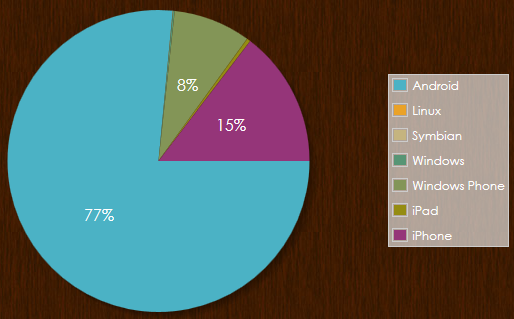
\includegraphics[keepaspectratio=true, width=12cm]{images/screenshots/statistics/app_plattform.png}
\caption{Plattform-App}
\label{fig:content_draft_log_app}
\end{figure}

In der Development Console von Google kann genau eingesehen werden, wann, welches Gerät, welche Android-Version, Land und Sprache die App installiert und deinstalliert hat. Somit ergaben sich die Zahlen, dass unsere App von 120 Personen heruntergeladen und davon haben sie momentan 91 Personen noch auf ihrem Gerät installiert. Die relativ große Differenz lässt sich dahingehend erklären, dass die App wahrscheinlich auch von Personen heruntergeladen wurde, welche die App nicht betrifft. Außerdem ist unsere App 20 mal bewertet worden und hat eine durchschnittliche Bewertung von 4,85 von maximalen 5 Punkten. In der \autoref{fig:content_draft_log_app_install} ist die Statistik zu sehen, wann die App installiert worden ist.

\begin{figure}[H]
\centering
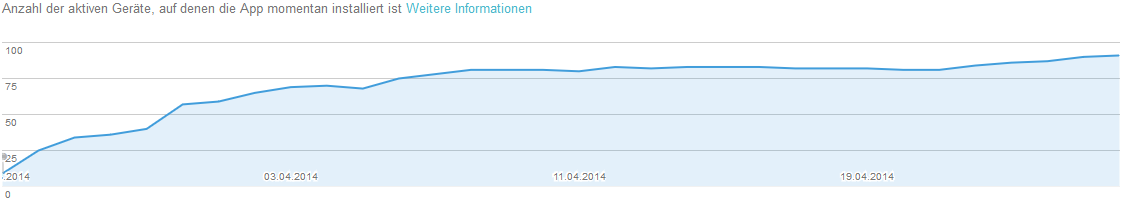
\includegraphics[keepaspectratio=true, width=17cm]{images/screenshots/statistics/app_install.png}
\caption{Plattform-App}
\label{fig:content_draft_log_app_install}
\end{figure}

\paragraph{PC\\}
Wie auch schon bei der App gibt es, wie erwartet, auch bei den PC Plattformen einen, weit abgeschlagenen, ersten Platz, was die Nutzung anbelangt. Dies ist natürlich Windows. In der \autoref{fig:content_draft_log_pc} ist zu sehen, dass sich eigentlich keine andere Plattform mit Windows messen kann. In der \autoref{fig:content_draft_log_pc} sind auch viele Mobile Betriebssysteme zu sehen, dies kann darauf zurückzuführen sein, dass viele dieser Geräte die Webseite besucht haben, dadurch werden sie auch in dieser Statistik gezählt. Diese Mobilen Geräte werden, bevor es die App gab, die Webseite benützt haben. Erstaunlich ist, dass Mac OSX vor Linux liegt.
\begin{figure}[H]
\centering
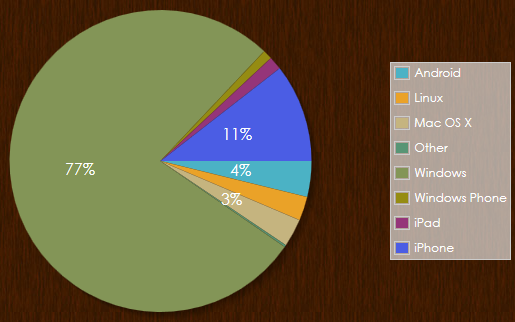
\includegraphics[keepaspectratio=true, width=12cm]{images/screenshots/statistics/pc_plattform.png}
\caption{Plattform-PC}
\label{fig:content_draft_log_pc}
\end{figure}

Firefox ist bei den Browsern auf unserer Webseite am meisten vertreten. Neben Firefox ist auch noch Safari Internet Explorer und Chrome zu nennen. Die sich die restlichen ca. 50 \% teilen. (siehe \autoref{fig:content_draft_log_pc_browser})

\begin{figure}[H]
\centering
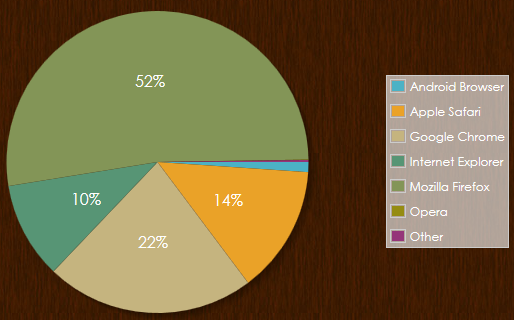
\includegraphics[keepaspectratio=true, width=12cm]{images/screenshots/statistics/pc_browser.png}
\caption{Browser-PC}
\label{fig:content_draft_log_pc_browser}
\end{figure}

\paragraph{App/PC\\}
Eine der interessantesten Statistik ist die Aufteilung der Seitenaufrufe zwischen App und PC. Wenn man bedenkt, dass die App wesentlich später den breiten Massen vorgeführt wurde, ist die App bei weitem attraktiver bei den Nutzern als der PC. Anfangs war die App dem PC unterlegen, als aber die App für Android und Windows Phone in Umlauf kam, holte die App immer weiter auf. Momentan liegt die App be 63 \% und der PC bei 37 \%. Die Tendenz der App zeigt jedoch nach oben. Vielleicht lässt sich dieses Phänomen auch daran erklären, dass man aus Langeweile eher kurz die App aufmacht die einzelnen Punkte durchsieht und sie wieder schließt, dies ist im Web nicht so leicht möglich. Deshalb sieht es im Moment so aus, dass die App, auf lange Sicht gesehen, das Web verdrängen wird.

\paragraph{Zugriffszeiten\\}
Interessant sind auch die Zugriffszeiten und die Anzahl der Seitenaufrufe pro Tag.\\
Mit diesen Diagrammen kann man die Zeiten herausfinden, an denen der Service am häufigsten genutzt wird. Das Ergebnis liefert, dass im Durchschnitt die Nutzung unseres Services um 7 Uhr beginnt und um 22 Uhr endet. In dieser Zeit kann man sehen, dass zwischen 7 und 8 Uhr die meisten Aufrufe getätigt werden. Dies nimmt dann stetig ab, bis zwischen 9 und 10 Uhr noch ein Maximum erreicht wird. Im Laufe des Tages nehmen die Aufrufe leicht ab, bis sie zwischen 16 und 17 Uhr ihr Minimum erreichen. Zwischen 12 und 13 Uhr ist nochmals eine Erhöhung zu sehen. Ab 17 Uhr steigen die Zahlen wieder und erreichen zwischen 21 - 22 Uhr das Maximum. (siehe \autoref{fig:content_draft_log_zugriff_std})

\begin{figure}[H]
\centering
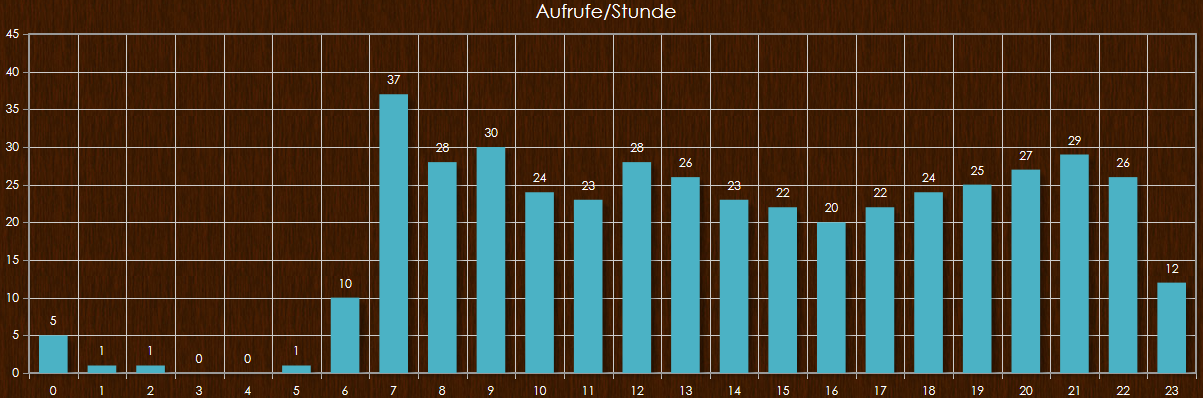
\includegraphics[keepaspectratio=true, width=17cm]{images/screenshots/statistics/aufruf_std.png}
\caption{Aufrufe/Stunde}
\label{fig:content_draft_log_zugriff_std}
\end{figure}

Wird der Zeitraum von einer Woche betrachtet, dann ist zu sehen, dass die Aufrufe während einer Woche sehr schwanken, sie sind jedoch jeden Tag in einem Bereich, wo man sagen kann, dass unser Service gut genutzt wird. Am Samstag kann beobachtet werden, dass am wenigsten Aufrufe zusammen kommen. Am Sonntag beginnen die Nutzer wieder den Service zu nutzen, dies sieht man an den steigenden Aufrufszahlen. Es konnte beobachtet werden, dass es immer wieder während den Wochentagen ein Ausreißer nach oben gibt, es konnte jedoch kein Muster erkannt werden. (siehe \autoref{fig:content_draft_log_zugriff_tag})


\begin{figure}[H]
\centering
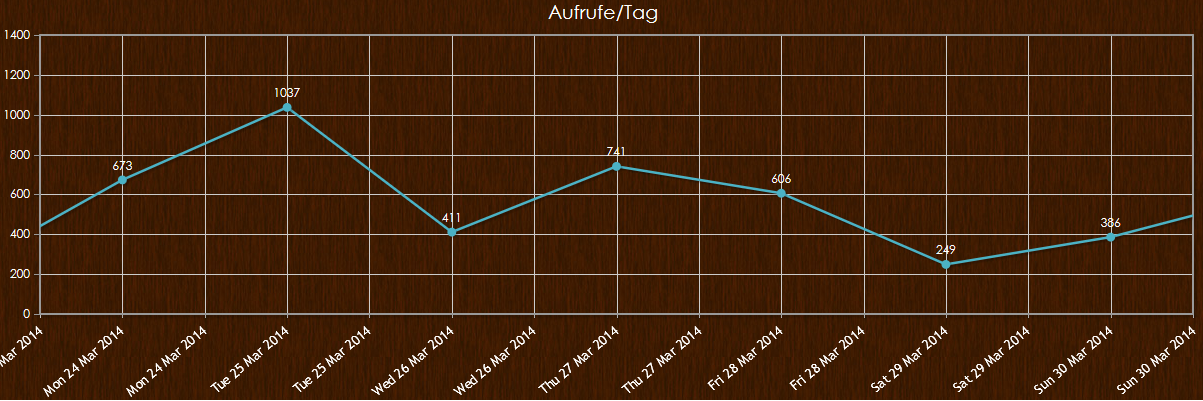
\includegraphics[keepaspectratio=true, width=17cm]{images/screenshots/statistics/aufruf_tag.png}
\caption{Aufrufe/Tag}
\label{fig:content_draft_log_zugriff_tag}
\end{figure}

\paragraph{Jahrgänge und Lehrer\\}
Ein sehr auffallendes Muster konnte bei der Aufteilung, von der Nutzung der einzelnen Jahrgängen und Lehrer, erkannt werden. Erstaunlich ist, dass der erste Jahrgang unseren Service wesentlich mehr nutzt, als alle anderen Jahrgänge. Außerdem nimmt die Nutzung unseres Services mit steigendem Jahrgang ab. Dies kann auf die sinkende Schülerzahl der Jahrgänge nach oben hin in Verbindung gebracht werden oder es kommt daher, dass die jüngere Generation öfters auf ihr Smartphone schaut oder im Web unterwegs ist.\\
Nach dem 1. Jahrgang kommen die Lehrer von der Nutzungshäufigkeit gesehen, dies ist wahrscheinlich darauf zurückzuführen, dass die Administratoren Lehrer sind und deshalb unseren Service wesentlich öfters nutzen. (siehe \autoref{fig:content_draft_log_jahr})

\begin{figure}[H]
\centering
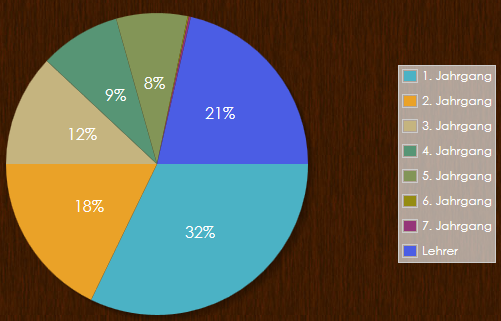
\includegraphics[keepaspectratio=true, width=12cm]{images/screenshots/statistics/jahrgang.png}
\caption{Aufrufe/Tag}
\label{fig:content_draft_log_jahr}
\end{figure}

%\section{Feinentwurf}

\newpage
\section{Implementierung}
\subsection{Basis-System}
Das Basissystem ist relativ simple gehalten.\\
\subsubsection{Konfiguration}
Die erste - und wohl auch wichtigste - Datei des Basis-Systems ist die Datei /config.php, diese soll unter anderem das Problem des Wurzelverzeichnisses lösen (siehe \gref{sec:content_solutions_root}).
\lstinputlisting[style=custom, language=php, caption={/config.php}, label={lst:content_imple_base_config}]{sources/base/config.php}
In dieser werden drei Konstanten definiert:
\begin{description}
	\item[\texttt{BETA}] ist \texttt{true} solange das System im Testbetrieb ist.
	\item\texttt{[RELATIVE\_ROOT}] beinhaltet den relativen Pfad vom Grundverzeichnis des virtuellen Hosts (vorgegeben durch den Webserver) zum Grundverzeichnis des Projektes. Hierbei ist zubachten, dass das erste Querstrich-Zeichen wegzulassen ist.\\
	\textit{Beispiel:} Ist das Grundverzeichnis des virtuellen Hosts bereits das Wurzelverzeichnis des Projektes, so muss der String "'"' verwendet werden.\\
	\textit{Beispiel:} Befindet sich das Projekt im Ordner \enquote{foobar} unterhalb des Grundverzeichnisses des virtuellen Hosts, so ist der betreffende String "'\texttt{foobar/}"'.
	\item[\texttt{ROOT\_LOCATION}] beinhaltet den absoluten Pfad vom Grundverzeichnis des Servers zum Projektverzeichnis. Dieser wird aus dem \texttt{DOCUMENT\_ROOT}, also dem Grundverzeichnis des virtuellen Hosts, und dem relativen Pfad des Projekt-Ordners zum \texttt{DOCUMENT\_ROOT} gebildet.
\end{description}

\subsubsection{Main-File}
Die quasi Hauptdatei des Basis-Systems stellt die Datei /modules/general/Main.php dar. Diese bindet weitere wichtige Dateien des Grundsystems ein, dies soll das Einbinden der wichtigsten Module erleichtern.
\lstinputlisting[style=custom, language=php, caption={/modules/general/Main.php; Zeilen 8-12},  label={lst:content_imple_base_main}, firstline=8, lastline=12, firstnumber=8]{sources/base/Main.php}
Es werden folgende Module des Basis-Systems eingebunden:
\begin{itemize}
	\item CheckCookies, siehe \autoref{sec:content_imple_base_cookie}
	\item ForceHTTPS, siehe \autoref{sec:content_imple_base_https}
	\item SessionManager, siehe \autoref{sec:content_imple_base_session}
	\item Connect, siehe \autoref{sec:content_imple_base_connect}
	\item Site, siehe \autoref{sec:content_imple_base_site}
\end{itemize}

\subsubsection{CheckCookie}
\label{sec:content_imple_base_cookie}
Das Modul CheckCookie prüft, ob die Cookies erlaubt sind, und leitet gegebenenfalls auf die Cookies-Akzeptieren-Seite (/cookies/) weiter. Zusätzlich wird das \enquote{Allow-Cookies}-Cookie erneuert (das Ablaufdatum wird 100 Tage in die Zukunft gesetzt).
\lstinputlisting[style=custom, language=php, caption={/modules/general/CheckCookie.php; Zeilen 9-13},  label={lst:content_imple_base_cookie}, firstline=9, lastline=13, firstnumber=9]{sources/base/CheckCookie.php}
Wie im Quellcode ersichtlich ist, wird die \texttt{REQUEST\_URI}, also die URL inklusive GET-Paremeter und Fragmentbezeichner der aktuellen Seite, der Cookies-Akzeptieren-Seite als GET-Parameter mitgegeben. Dies dient dazu, dass die Cookies-Akzeptieren-Seite den Benutzer nach dem Akzeptieren wieder auf die ursprüngliche Seite zurückschicken kann.
%
%
% \lstinputlisting[style=custom, language=php, caption={Dateiname}, label={lst:content_imple_timetables_labelname}]{sources/ordner/datei.php}
%
% Als weitere Eigenschaft kannst du die Zeilen angeben: [firstline=300, lastline=500]
% Damit nicht alles reinkopiert wird.
\subsection{Datenbank}
% Implementierung der Datenbank
Die Implementierung der Datenbank wurde mit dem gratis erhältlichen Tool \textit{phpMyAdmin} vorgenommen. Unsere Wahl viel auf dieses Tool, da es einfach zu verwenden ist und nicht installiert werden muss. Die andere Möglichkeit wäre gewesen, dass wir die Datenbank mittels \textit{PHP} erstelle, dies hätte jedoch wesentlich mehr Zeit benötigt. Eine andere Möglichkeit wäre gewesen, dass wir mittels SSH und dem Kommandozeilen-Tool für MySQL die Datenbank erstellt hätten, dies war uns jedoch nicht möglich, da wir keinen SSH-Zugriff bekamen.
\subsubsection{Aufbau}
% Genaue Auflistung der Tabellen, Spalten, Kommentare, etc.
%
% @marco: Du hast das ja gemacht. Willst du das schreiben?
% Ich würde sagen, du schreibst da einfach, bis dir nichts mehr einfällt, und dann mentionst du mich in einem commit und ich schreib weiter.
Wie schon im \autoref{sec:content_solution_db} aufgelistet wurden die Tabellen dementsprechend erstellt. In diesem Abschnitt werden die Tabellen mit ihren Spalten und Datentypen aufgelistet.\\

\paragraph{Klassen\\}
In dieser Tabelle werden alle Klassen gespeichert. Der Tabellenname lautet \textit{classes}. Diese Tabelle umfasst insgesamt 6 Spalten.
\begin{table}[H]
\centering
\begin{tabular}{p{2.5 cm}p{2.5 cm}p{10 cm}}
   \toprule
   \textbf{Spalte} & \textbf{Datentyp} & \textbf{Beschreibung} \\
   \midrule
          ID & Integer & Auto increment - Primärschlüssel  \\
          \hline
          name & Text & Name der Klasse \\
          \hline
          sectionFK & Integer & Fremdschlüssel auf die Abteilungs-Tabelle \\
          \hline
          teacherFK & Integer & Fremdschlüssel auf die Lehrer-Tabelle\\
          \hline
          roomFK & Integer & Fremdschlüssel auf die Raum-Tabelle\\
          \hline
          invisible & Boolean & Ob Eintrag sichtbar oder nicht\\
   \bottomrule
\end{tabular}
\caption{Klassen-Tabelle}
\end{table}

\paragraph{Display-Modus\\}
In dieser Tabelle sind die Modi für die Ein- und Ausschaltzeiten für die Monitore gespeichert. Der Tabellenname lautet \textit{displayMode}. Diese Tabelle umfasst insgesamt 2 Spalten.
\begin{table}[H]
\centering
\begin{tabular}{p{2.5 cm}p{2.5 cm}p{10 cm}}
   \toprule
   \textbf{Spalte} & \textbf{Datentyp} & \textbf{Beschreibung} \\
   \midrule
          ID & Integer & Auto increment - Primärschlüssel  \\
          \hline
          name & Text & Name des Modus \\
   \bottomrule
\end{tabular}
\caption{Display-Modus-Tabelle}
\end{table}

\paragraph{Stunden\\}
In dieser Tabelle werden alle Stunden gespeichert, mit deren Anfangs- und Endzeiten. Um nicht zusätzlich die Wochentage speichern zu müssen, werden dise zu den Stunden gespeichert. Deshalb ist eine gewisse Redundanz der Zeiten gegeben, diese nahmen wir jedoch in kauf. Zu einem Problem wird dies dann, wenn sich zum Beispiel eine Uhrzeit ändern sollte. Der Tabellenname lautet \textit{hours}. Diese Tabelle umfasst insgesamt 6 Spalten.
\begin{table}[H]
\centering
\begin{tabular}{p{2.5 cm}p{2.5 cm}p{10 cm}}
   \toprule
   \textbf{Spalte} & \textbf{Datentyp} & \textbf{Beschreibung} \\
   \midrule
          ID & Integer & Auto increment - Primärschlüssel  \\
          \hline
          weekday & Text & Wochentag - z.B.: Montag  \\
          \hline
          weekdayShort & Text & Wochentag-Kürzel z.B.: Mo   \\
          \hline
          hour & Integer & Stunde z.B: 1 oder 12  \\
          \hline
          startHour & Time & Anfangsstunde z.B.: 8:00  \\
          \hline
          endHour & Time & Endstunde z.B.: 8:50 \\
   \bottomrule
\end{tabular}
\caption{Stunden-Tabelle}
\end{table}

\paragraph{Stundenplan\\}
Für den Stundenplan sind 2 Tabellen notwendig. In einer Tabelle werden die Basisstunden einer Klasse gespeichert. In der anderen Tabelle werden die Baisstunden mit den anderen Informationen verknüpft. (siehe \autoref{sec:content_solution_db})

\subparagraph{Basis-Stundenplan\\}
In dieser Tabelle werden die Basisstunden gespeichert. Der Tabellenname lautet \textit{lessonsBase}. Diese Tabelle umfasst insgesamt 4 Spalten.

\begin{table}[H]
\centering
\begin{tabular}{p{2.5 cm}p{2.5 cm}p{10 cm}}
   \toprule
   \textbf{Spalte} & \textbf{Datentyp} & \textbf{Beschreibung} \\
   \midrule
          ID & Integer & Auto increment - Primärschlüssel  \\
          \hline
          classFK & Integer & Fremdschlüssel auf die Klassen-Tabelle   \\
          \hline
          startHourFK & Integer & Fremdschlüssel auf die Stunden-Tabelle  \\
          \hline
          endHourFK & Integer & Fremdschlüssel auf die Stunden-Tabelle  \\
   \bottomrule
\end{tabular}
\caption{Basis-Stundenplan-Tabelle}
\end{table}

\subparagraph{Eigentlicher Stundenplan\\}
In dieser Tabelle werden die Basisstunden mit zusätzlichen Informationen zusammengeführt und gespeichert. Der Tabellenname lautet \textit{lessons}. Diese Tabelle umfasst insgesamt 6 Spalten.

\begin{table}[H]
\centering
\begin{tabular}{p{2.5 cm}p{2.5 cm}p{10 cm}}
   \toprule
   \textbf{Spalte} & \textbf{Datentyp} & \textbf{Beschreibung} \\
   \midrule
          ID & Integer & Auto increment - Primärschlüssel  \\
          \hline
          lessonBaseFK & Integer & Fremdschlüssel auf die Basis-Stundenplan-Tabelle   \\
          \hline
	      roomFK & Integer & Fremdschlüssel auf die Raum-Tabelle   \\
	      \hline
          teachersFK & Integer & Fremdschlüssel auf die Lehrer-Tabelle   \\
          \hline
          subjectFK & Integer & Fremdschlüssel auf die Fächer-Tabelle  \\
          \hline
          comment & Text & Kommentar zur Stunde  \\
   \bottomrule
\end{tabular}
\caption{Stundenplan-Tabelle}
\end{table}

\paragraph{Logs\\}
Für das Speichern der Logs wurden insgesamt 5 Tabellen benötigt, welche teilweise miteinander verknüpft werden.

\subparagraph{Logins\\}
In dieser Tabelle werden jegliche Anmeldeversuche an unsere Seite gespeichert. Außerdem wird hier auch gespeichert, ob die Anmeldung fehlschlug oder funktionierte. Der Tabellenname lautet \textit{logsLogins}. Diese Tabelle umfasst insgesamt 6 Spalten.

\begin{table}[H]
\centering
\begin{tabular}{p{2.5 cm}p{2.5 cm}p{10 cm}}
   \toprule
   \textbf{Spalte} & \textbf{Datentyp} & \textbf{Beschreibung} \\
   \midrule
          ID & Integer & Auto increment - Primärschlüssel  \\
          \hline
          time & Integer & Zeit als Unix-Timestamp   \\
          \hline
	      user & Text & Loginname   \\
	      \hline
          userAgent & Text & User Agent des Browsers   \\
          \hline
          ip & Text & IP-Adresse  \\
          \hline
          success & Integer & 1-Erfolgreich; 0-Nicht Erfolgreich  \\
   \bottomrule
\end{tabular}
\caption{Logins-Tabelle}
\end{table}

\subparagraph{Basis-Log\\}
In dieser Tabelle werden die Log-Informationen miteinander verknüpft. Hier werden alle Bewegungen in der Seite einer Session zugewiesen. Der Tabellenname lautet \textit{logsMain}. Diese Tabelle umfasst insgesamt 5 Spalten.

\begin{table}[H]
\centering
\begin{tabular}{p{2.5 cm}p{2.5 cm}p{10 cm}}
   \toprule
   \textbf{Spalte} & \textbf{Datentyp} & \textbf{Beschreibung} \\
   \midrule
          ID & Integer & Auto increment - Primärschlüssel  \\
          \hline
          time & Integer & Zeit als Unix-Timestamp   \\
          \hline
	      connFK & Integer & Fremdschlüssel auf die \textit{logsUSConn}-Tabelle   \\
	      \hline
          site & Text & Aufgerufene Seite   \\
          \hline
          params & Text & Angehängte Parameter an die URL  \\
   \bottomrule
\end{tabular}
\caption{Basis-Log-Tabelle}
\end{table}

\subparagraph{User-Session-Log\\}
Da ein User mehrere Sessions und eine Session hintereinander mehrere User haben kann, musste eine Verbindungstabelle dieser beiden Informationen erstellt werden. Diese Daten werden in dieser Tabelle gespeichert. Der Tabellenname lautet \textit{logsUSConn}. Die Tabelle umfasst insgesamt 5 Spalten.

\begin{table}[H]
\centering
\begin{tabular}{p{2.5 cm}p{2.5 cm}p{10 cm}}
   \toprule
   \textbf{Spalte} & \textbf{Datentyp} & \textbf{Beschreibung} \\
   \midrule
          ID & Integer & Auto increment - Primärschlüssel  \\
          \hline
          time & Integer & Zeit als Unix-Timestamp   \\
          \hline
	      sessionFK & Integer & Fremdschlüssel auf die Session-Logs-Tabelle   \\
	      \hline
          userFK & Integer & Fremdschlüssel auf die User-Logs-Tabelle   \\
          \hline
          ip & Text & IP-Adresse  \\
   \bottomrule
\end{tabular}
\caption{User-Session-Tabelle}
\end{table}

\subparagraph{Session-Log\\}
Alle eröffneten Sessions mit dem Server werden hier gespeichert. Diese werden später in der Tabelle \textit{logsUSConn} mit dem User zusammengeführt. Der Tabellenname lautet \textit{logsSessions}. Die Tabelle umfasst insgesamt 5 Spalten.

\begin{table}[H]
\centering
\begin{tabular}{p{2.5 cm}p{2.5 cm}p{10 cm}}
   \toprule
   \textbf{Spalte} & \textbf{Datentyp} & \textbf{Beschreibung} \\
   \midrule
          ID & Integer & Auto increment - Primärschlüssel  \\
          \hline
          time & Integer & Zeit als Unix-Timestamp   \\
          \hline
	      PhpSessIDOrig & Text & Erste Session ID   \\
	      \hline
          userAgent & Text & User Agent des Browsers   \\
          \hline
          PhpSessIDAct & Text & Aktuelle Session ID  \\
   \bottomrule
\end{tabular}
\caption{Session-Tabelle}
\end{table}

\subparagraph{User-Log\\}
In dieser Tabelle werden die User gespeichert, welche unsere Seite besuchen. Um bei den Statistiken, ohne LDAP-Abfrage, zu erkennen welcher Abteilung/Klasse ein Schüler angehört, speichern wir in diesem Zusammenhang die Klasse und die Abteilung des Schülers. Der Tabellenname lautet \textit{logsUsers}. Diese Tabelle umfasst insgesamt 5 Spalten. 

\begin{table}[H]
\centering
\begin{tabular}{p{2.5 cm}p{2.5 cm}p{10 cm}}
   \toprule
   \textbf{Spalte} & \textbf{Datentyp} & \textbf{Beschreibung} \\
   \midrule
          ID & Integer & Auto increment - Primärschlüssel  \\
          \hline
          LDPA & Text & LDAP-ID des Schülers/Lehrers   \\
          \hline
	      classesFK & Integer & Fremdschlüssel auf die Klassen-Tabelle   \\
	      \hline
          sectionsFK & Integer & Fremdschlüssel auf die Abteilungs-Tabelle   \\
          \hline
          isTeacher & Integer & 1-Ja, 0-Nein  \\
   \bottomrule
\end{tabular}
\caption{User-Session-Tabelle}
\end{table}

\paragraph{Fehlende Klassen\\}
In dieser Tabelle werden die als fehlend eingetragenen Klassen gespeichert. Der Tabellenname lautet \textit{missingClasses}. Die Tabelle umfasst insgesamt 7 Spalten.

\begin{table}[H]
\centering
\begin{tabular}{p{2.5 cm}p{2.5 cm}p{10 cm}}
   \toprule
   \textbf{Spalte} & \textbf{Datentyp} & \textbf{Beschreibung} \\
   \midrule
          ID & Integer & Auto increment - Primärschlüssel  \\
          \hline
          classFK & Integer & Fremdschlüssel auf die Klassen-Tabelle   \\
          \hline
	      startDay & Date & Datum des Starttages   \\
	      \hline
          startHourFK & Integer & Fremdschlüssel auf die Stunden-Tabelle   \\
          \hline
          endDay & Date & Datum des Endtages   \\
          \hline
          endHourFK & Integer & Fremdschlüssel auf die Stunden-Tabelle   \\
          \hline
          reason & Text & Grund des Fehlens  \\
   \bottomrule
\end{tabular}
\caption{Fehlende-Klasse-Tabelle}
\end{table}

\paragraph{Fehlende Lehrer\\}
In dieser Tabelle werden die als fehlend eingetragenen Lehrer gespeichert. Der Tabellenname lautet \textit{missingTeachers}. Die Tabelle umfasst insgesamt 7 Spalten.

\begin{table}[H]
\centering
\begin{tabular}{p{2.5 cm}p{2.5 cm}p{10 cm}}
   \toprule
   \textbf{Spalte} & \textbf{Datentyp} & \textbf{Beschreibung} \\
   \midrule
          ID & Integer & Auto increment - Primärschlüssel  \\
          \hline
          teacherFK & Integer & Fremdschlüssel auf die Lehrer-Tabelle   \\
          \hline
	      startDay & Date & Datum des Starttages   \\
	      \hline
          startHourFK & Integer & Fremdschlüssel auf die Stunden-Tabelle   \\
          \hline
          endDay & Date & Datum des Endtages   \\
          \hline
          endHourFK & Integer & Fremdschlüssel auf die Stunden-Tabelle   \\
          \hline
          reason & Text & Grund des Fehlens  \\
   \bottomrule
\end{tabular}
\caption{Fehlende-Lehrer-Tabelle}
\end{table}

\paragraph{Monitor Modus\\}
In dieser Tabelle werden die verschiedenen Betriebsarten des Monitors gespeichert. Der Tabellenname lautet \textit{monitorMode}. Diese Tabelle umfasst insgesamt 2 Spalten.

\begin{table}[H]
\centering
\begin{tabular}{p{2.5 cm}p{2.5 cm}p{10 cm}}
   \toprule
   \textbf{Spalte} & \textbf{Datentyp} & \textbf{Beschreibung} \\
   \midrule
          ID & Integer & Auto increment - Primärschlüssel  \\
          \hline
          name & Text & Name des Modus  \\
   \bottomrule
\end{tabular}
\caption{Monitor-Modus-Tabelle}
\end{table}

\paragraph{Fehlende Lehrer\\}
In dieser Tabelle sind alle Moonitore eingetragen, die in SIS registriet werden. Die Zuteilung der verschiedenen Modi wird in dieser Tabelle gespeichert. Der Tabellenname lautet \textit{monitors}. Die Tabelle umfasst insgesamt 12 Spalten.

\begin{table}[H]
\centering
\begin{tabular}{p{3.5 cm}p{2.5 cm}p{9.5 cm}}
   \toprule
   \textbf{Spalte} & \textbf{Datentyp} & \textbf{Beschreibung} \\
   \midrule
          ID & Integer & Auto increment - Primärschlüssel  \\
          \hline
          name & Text & Name des Monitors   \\
          \hline
	      text & Text & Text der am Monitor links unten angezeigt wird  \\
	      \hline
          modeFK & Integer & Fremdschlüssel auf die Monitor-Modus-Tabelle   \\
          \hline
          file & Text & Dateinamen der zugewiesenen Datei    \\
          \hline
          roomFK & Integer & Fremdschlüssel auf die Raum-Tabelle   \\
          \hline
          sectionFK & Integer & Fremdschlüssel auf die Abteilungs-Tabelle   \\
          \hline
	      time & Integer & Erstellzeit als Unix-Timestamp   \\
	      \hline
          displayModeFK & Integer & Fremdschlüssel auf die Display-Modus-Tabelle   \\
          \hline
          displayStartDaytime & Integer & Unix-Timestamp der Einschaltzeit   \\
          \hline
          siplayEndDaytime & Integer & Unix-Timestamp der Ausschaltzeit   \\
          \hline                    	      
          ip & Text & IP Adresse beim Erstellen  \\
   \bottomrule
\end{tabular}
\caption{Monitor-Tabelle}
\end{table}

\paragraph{Räume\\}
In dieser Tabelle werden die Räume gespeichert. Der Tabellenname lautet \textit{rooms}. Diese Tabelle umfasst 3 Spalten.

\begin{table}[H]
\centering
\begin{tabular}{p{2.5 cm}p{2.5 cm}p{10 cm}}
   \toprule
   \textbf{Spalte} & \textbf{Datentyp} & \textbf{Beschreibung} \\
   \midrule
          ID & Integer & Auto increment - Primärschlüssel  \\
          \hline
          name & Text & Name des Raumes  \\
          \hline        
          teacherFK & Integer & Fremdschlüssel auf die Lehrer-Tabelle \\
   \bottomrule
\end{tabular}
\caption{News-Tabelle}
\end{table}

\paragraph{Abteilungen\\}
In dieser Tabelle werden die Abteilungen gespeichert. Der Tabellenname lautet \textit{sections}. Die Tabelle umfasst 4 Spalten.

\begin{table}[H]
\centering
\begin{tabular}{p{2.5 cm}p{2.5 cm}p{10 cm}}
   \toprule
   \textbf{Spalte} & \textbf{Datentyp} & \textbf{Beschreibung} \\
   \midrule
          ID & Integer & Auto increment - Primärschlüssel  \\
          \hline
          name & Text & Name der Abteilung   \\
          \hline
	      short & Text & Abteilungskürzel   \\
	      \hline
          teacherFK & Integer & Fremdschlüssel auf die Lehrer-Tabelle   \\
   \bottomrule
\end{tabular}
\caption{Abteilungs-Tabelle}
\end{table}

\paragraph{Fächer\\}
In dieser Tabelle werden alle Fächer gespeichert. Der Tabellenname lautet \textit{subjects}. Die Tabelle umfasst 4 Spalten.

\begin{table}[H]
\centering
\begin{tabular}{p{2.5 cm}p{2.5 cm}p{10 cm}}
   \toprule
   \textbf{Spalte} & \textbf{Datentyp} & \textbf{Beschreibung} \\
   \midrule
          ID & Integer & Auto increment - Primärschlüssel  \\
          \hline
          name & Text & Name des Faches   \\
          \hline
	      short & Text & Fächer-Kurzbezeichnung   \\
	      \hline
          invisible & Boolean & Ob Eintrag sichtbar oder nicht   \\
   \bottomrule
\end{tabular}
\caption{Fächer-Tabelle}
\end{table}

\paragraph{Fehlende Lehrer\\}
In dieser Tabelle werden alle Supplierungen gespeichert. Der Tabellenname lautet \textit{substitudes}. Die Tabelle umfasst insgesamt 13 Spalten.

\begin{table}[H]
\centering
\begin{tabular}{p{2.5 cm}p{2.5 cm}p{10 cm}}
   \toprule
   \textbf{Spalte} & \textbf{Datentyp} & \textbf{Beschreibung} \\
   \midrule
          ID & Integer & Auto increment - Primärschlüssel  \\
          \hline
          time & Date & Datum der Supplierung   \\
          \hline
	      newSub & Integer & Ob die Stunde hinzugefügt wird  \\
	      \hline
          remove & Boolean & Ob die Stunde entfernt wird   \\
          \hline
          lessonFK & Integer & Fremdschlüssel auf die Stundenplan-Tabelle    \\
          \hline
          startHourFK & Integer & Fremdschlüssel auf die Stunden-Tabelle   \\
          \hline
          endHourFK & Integer & Fremdschlüssel auf die Stunden-Tabelle   \\
          \hline
	      teacherFK & Integer & Fremdschlüssel auf die Lehrer-Tabelle \\
	      \hline
          subjectFK & Integer & Fremdschlüssel auf die Fächer-Tabelle   \\
          \hline
          roomFK & Integer & Fremdschlüssel auf die Raum-Tabelle \\
          \hline
          classFK & Integer & Fremdschlüssel auf die Klassen-Tabelle \\
          \hline    
          comment & Text & Kommentar \\
          \hline                 	      
          move & Boolean & Ob die Stunde verschoben wird  \\
   \bottomrule
\end{tabular}
\caption{Supplierungs-Tabelle}
\end{table}

\paragraph{Lehrer\\}
In dieser Tabelle werden alle Lehrer gespeichert. Der Tabellenname lautet \textit{teachers}. Die Tabelle umfasst insgesamt 6 Spalten.

\begin{table}[H]
\centering
\begin{tabular}{p{2.5 cm}p{2.5 cm}p{10 cm}}
   \toprule
   \textbf{Spalte} & \textbf{Datentyp} & \textbf{Beschreibung} \\
   \midrule
          ID & Integer & Auto increment - Primärschlüssel  \\
          \hline
          name & Text & Name des Lehrers \\
          \hline
	      short & Text & Lehrerkürzel   \\
	      \hline
          display & Text & Kurzname des Lehrers   \\
          \hline
          sectionFK & Integer & Fremdschlüssel auf die Abteilungs-Tabelle   \\
          \hline
          invisible & Boolean & Ob Eintrag sichtbar oder nicht \\
   \bottomrule
\end{tabular}
\caption{Lehrer-Tabelle}
\end{table}

\subsubsection{Zugriff}
% Ich weiß nicht, ob es bekannt war, aber es gab eine Home-Made Lib für den Datenbankzugriff von Marco
% Die könnte man hier dokumentieren.
% 
Für die Datenbankanbindung siehe \gref{sec:content_imple_base_connect}.\\
Für die Eingaben wurden in einer selbst erstellten Libary \textit{selects} und \textit{inserts} entwickelt. Die Select-Funktionen befinden sich in der Datei \textit{/modules/databse/selects.php}. Die Insert-Befehle befinden sich in der Datei \textit{/modules/database/inserts.php}. Diese Zeilen können in der Formular-Datei inkludiert werden, dann sind alle Funktionen verfügbar. (siehe \autoref{lst:content_imple_data_include_bsp})

\lstinputlisting[style=custom, language=php, caption={/backend/administration/teachers/index.php; Zeile 17 - 18},  label={lst:content_imple_data_include_bsp}, firstline =17, lastline = 18, firstnumber = 17 ]{sources/input/teacher.php}

Ein Funktionsaufruf für die Select-Funktion des Lehrer-Formulars sieht wie in \autoref{lst:content_imple_data_select} zu sehen aus. In Zeile 53 wird eine Sortierung für die Datensätze definiert, welche in Zeile 54 der Funktion mitgegeben wird. In Zeile 54 wird das Ergebnis der Funktion in eine Variable gespeichert.

\lstinputlisting[style=custom, language=php, caption={/backend/administration/teachers/index.php; Zeile 53 - 54},  label={lst:content_imple_data_select}, firstline =53, lastline = 54, firstnumber = 53 ]{sources/input/teacher.php}

Ein Funktionsaufruf für die Insert-Funktion des Lehrer-Formulars sieht wie in \autoref{lst:content_imple_data_insert} zu sehen aus. In der Zeile 29 wird in einer \textit{If}-Abfrage abgefragt, ob im Formular übernehmen geklickt wurde. In der Zeile 31 wird die Insert-Funktion aufgerufen. Die Zeile 30 ruft eine Funktion auf, um zu kontrollieren, ob das Formular gültig ist.

\lstinputlisting[style=custom, language=php, caption={/backend/administration/teachers/index.php; Zeile 29 - 32},  label={lst:content_imple_data_insert}, firstline =29, lastline = 32, firstnumber = 29 ]{sources/input/teacher.php}

Im Folgenden werden die Funktionen genauer erklärt.

\subsubsection{Select-Funktionen}
Alle Select-Funktionen sind nach dem selben Prinzip aufgebaut. Neben den spezifischen Selects für die einzelnen Anforderungen wurde eine allgemeine Select-Funktion entwickelt.
\paragraph{SelectAll\\}
Dieser Funktion müssen 3 Parameter mitgegeben werden. Mit dem \texttt{\$table}-Parameter wird die Tabelle ausgewählt. Mit dem \texttt{\$where}-Parameter kann das Ergebnis eingegrenzt werden und mit dem \texttt{\$order}-Parameter kann die Sortierung der Ergebnisses verändert werden.\\
Diese Funktion ist im \autoref{lst:content_imple_select_all} zu sehen. In der Zeile 20 wird der Stamm SQL-Befehl mit der Tabelle-definiert. In den Zeilen 22 - 23 wird, falls die Parameter nicht leer sind, ein \textit{where} oder \textit{order by} Argument angehängt. In der Zeile 25 wird der SQL-Befehl ausgeführt und der Rückgabewert wird unbearbeitet zurückgegeben.

\lstinputlisting[style=custom, language=php, caption={/modules/database/selects.php; Zeile 18 - 26},  label={lst:content_imple_select_all}, firstline =18, lastline = 26, firstnumber = 18 ]{sources/database/selects.php}

\paragraph{Standard-Select\\}
Alle anderen Select-Funktionen sind gleich aufgebaut, sie unterscheiden sich jeweils nur am Stamm-SQL-Befehl. Diesen Funktionen muss der Tabellennam nicht mehr als Parameter übergeben werden. Die 2 anderen Parameter erfüllen die selbe Funktion wie in der \texttt{selectAll}-Funktion.\\
Der Aufbau der Funktion entspricht exakt, dem der \texttt{selectAll}-Funktion. Lediglich der Stamm-SQL-Befehl ist nicht mehr von der Tabelle abhängig, denn diese ist einprogrammiert. (siehe \autoref{lst:content_imple_select_std})

\lstinputlisting[style=custom, language=php, caption={/modules/database/selects.php; Zeile 76 - 86},  label={lst:content_imple_select_std}, firstline =76, lastline = 86, firstnumber = 76 ]{sources/database/selects.php}

\subsubsection{Insert-Funktionen}
Einige der Insert-Funktionen sind gleich aufgebaut. Für Spezialfälle mussten jedoch neue entwickelt werden. In diesem Abschnitt wird eine Standard-Insert-Funktion erläutert. Außerdem werden auch die stark abgeänderten Funktionen erläutert.

\paragraph{Allgemeine Insert-Funktion\\}
Die allgemeine Insert-Funktion wird anhand der Insert-Funktion für das Klassen-Formular erläutert.(siehe \autoref{lst:content_imple_insert_std})\\
Dieser Funktion muss kein Parameter mitgegeben werden, denn die Funktion hat Zugriff auf die \textit{POST}-Parameter. Diese werden in der Zeile 17 in eine dementsprechende Variable geschrieben. In der Zeile 20 wird der \textit{Save}-Parameter aus dem Array gelöscht.\\
In der Zeile 23 wird ein Array definiert, welches als Indizes die Spaltennamen der Tabelle hat, in die die Daten eingefügt werden. Die Indizes bekommen als Werte die Werte zugewiesen, welche in die Tabelle eingefügt werden sollten.\\
In der Zeile 25 wird die ID in das Array geschrieben, wenn es ein Update ist, gibt es eine ID, andernfalls ist diese leer. In den Zeilen 28 - 46 wird das Array vervollständigt.\\
Dabei gibt es zwei verschiedene Varianten:
\begin{itemize}
	\item Die Werte werden direkt aus dem \textit{POST}-Array übernommen und in das Array geschrieben. (siehe Zeile 28)
	\item Die Werte aus dem \textit{POST}-Array werden zuerst, in der dementsprechenden Tabelle, in eine zugehörige ID \enquote{umgewnandelt}. Dies ist nötig, weil wir die Tabellen miteinander verbinden und mittels ID auf andere Tabellen verweisen.\\
	In Zeile 36 ist die Abfrage für die ID zu sehen. In Zeile 38 wird der Rückgabewert mit der Funktion \texttt{control()} überprüft, dieser Rückgabewert wird in eine Variable gespeichert. Anschließend wird in Zeile 40 der Wert in das Array geschrieben. (Funktion \texttt{control} siehe Abschnitt \nameref{sec:content_imple_control})
\end{itemize}
In diesem Formular gibt es eine Check Box, bei dieser kann nicht einfach der Wert in das Array geschrieben werden, da in die Datenbank ein True oder False geschrieben werden muss. Bei aktivierter Check Box wird jedoch der Name der Check Box zurückgegeben. Darum muss in Zeile 49 geprüft werden, ob das Array-Element leer ist. Ist es nicht leer muss dem Array True zugewiesen werden.\\
In der Zeile 53 wird geprüft, ob bei Löschen ein Hacken im Formular gesetzt wurde und ob bei allen Überprüfungen 1 in die Variablen geschrieben wurde. Ist die Multiplikation der Kontroll-Variablen 1, dann ist alles korrekt abgelaufen und der Datensatz kann in der Zeile 54 eingefügt werden. (Funktion \texttt{saveupdate} siehe Abschnitt \nameref{sec:content_imple_saveupdate})

\lstinputlisting[style=custom, language=php, caption={/modules/database/inserts.php; Zeile 14 - 55},  label={lst:content_imple_insert_std}, firstline =14, lastline = 55, firstnumber = 14 ]{sources/database/inserts.php}

\paragraph{Insert Supplierplan\\}
Für den Supplierplan musste eine sehr aufwendige Funktion geschrieben werden, da es darauf ankommt welcher Eingabemodus, bei der Eingabe der Supplierungen, ausgewählt wurde. Um in dem Formular zu erkennen, ob das Hinzufügen in die Datenbank funktioniert hat, wird in dieser Funktion im Erfolgsfall ein True zurückgegeben, sonst ein False. Die grundsätzliche Zuweisung der Werte dem Array, das zum Speichern in der Datenbank verwendet wird, wird hier nicht weiter erklärt, denn diese funktioniert nach dem selben Prinzip wie oben erklärt. Hier werden nur die wesentlichen Unterschiede beschrieben. Diese Funktion wird in verschieden Teile zerlegt, um sie zu erklären.\\
\begin{enumerate}
\item \autoref{lst:content_imple_insert_suppl_1}\\
Bei der Insert-Funktion der Supplierungen werden keine vorhandenen Einträge, bei einem aktualisieren eines Eintrages, verändert, sondern der Eintrag wird gelöscht und anschließend neu erstellt. In Zeile 295 wird abgefragt, ob der Eintrag eine ID hat, wenn ja, wird ein bestehender Eintrag aktualisiert. Wenn nicht, dann ist es ein neuer Eintrag. Bei einem bestehendem Eintrag wird diese in dn Zeilen 298 - 299 gelöscht. Anschließend muss noch die alte ID aus dem Array gelöscht werden, dies wird in Zeile 300 durchgeführt. 

\lstinputlisting[style=custom, language=php, caption={/modules/database/inserts.php; Zeile 295 - 302},  label={lst:content_imple_insert_suppl_1}, firstline =295, lastline = 302, firstnumber = 295 ]{sources/database/inserts.php}

\item \autoref{lst:content_imple_insert_suppl_2}\\
Ist bei Löschen im Formular ein Hacken gesetzt worden, dann wird der restliche Code in der Funktion übersprungen. Dies wird mit der \textit{If}-Bedingung in der Zeile 304 durchgeführt.\\
In den Zeilen 306 - 308 entscheidet sich um welche Eingabemethode es sich handelt. Dafür sind \textit{If}-Abfragen zuständig, die weiteren Abfragen für die restlichen Eingabemethoden sind hier nicht dargestellt.

\lstinputlisting[style=custom, language=php, caption={/modules/database/inserts.php; Zeile 304 - 308},  label={lst:content_imple_insert_suppl_2}, firstline =304, lastline = 308, firstnumber = 304 ]{sources/database/inserts.php}

\item \autoref{lst:content_imple_insert_suppl_3}\\
Dies ist ein Ausschnitt aus dem Verarbeitungscode für den Entfall einer Stunde. Dabei wird das Array wie gewohnt befüllt, jedoch muss anschließend die Stunde, für die der Entfall eingetragen werden soll, gefunden werden. Dabei müssen 2 Fälle unterschieden werden, zum Einen es wird ein Lehrer mitgegeben, zum Anderen es wird kein Lehrer mitgegeben.\\
Diese Abfrage ist in Zeile 359 zu sehen. Der erste Teil wird abgearbeitet wenn kein Lehrer mitgegeben wird, denn dann werden alle Lehrer ausgewählt. Mit der SQL-Abfrage in den Zeilen 361 - 367 werden alle Stunden der Lehrer abgefragt, welche dieser Entfall betrifft. In Zeile 368 wird geprüft, ob Stunden gefunden wurden, wenn nicht wird False zurückgegeben. Wenn Stunden gefunden wurden, wird in Zeile 369 - 372 für jede Stunde eine Supplierung eingetragen.\\
Im zweiten Teil wird eine Supplierung für einen bestimmten Lehrer eingetragen. In den Zeilen 380 - 383 wird die Stunde des Lehrers abgefragt. In den Zeilen 385 - 388 wird eine Supplierung für diesen Lehrer eingetragen. Dies geschieht nur, wenn eine Stunde zu diesem Lehrer gefunden wurde, dies wird in der Zeile 385 überprüft. Ist keine gefunden worden, so wird ein False zurückgegeben.\\
Dieser Teil ist ebenfalls bei der Verschiebung vorhanden.

\lstinputlisting[style=custom, language=php, caption={/modules/database/inserts.php; Zeile 359 - 389},  label={lst:content_imple_insert_suppl_3}, firstline =359, lastline = 389, firstnumber = 359 ]{sources/database/inserts.php}

\item \autoref{lst:content_imple_insert_suppl_4}\\
In der freien Eingabe muss auf die Stunde mittels der fehlenden Lehrer zurück geschlossen werden. Dazu werden hier die möglichen fehlenden Lehrer, mit einer SQL-Abfrage in Zeile 488 - 493, abgefragt. Die abgefragten Daten werden in den Zeilen 495 - 497 in ein Array geschrieben.

\lstinputlisting[style=custom, language=php, caption={/modules/database/inserts.php; Zeile 488 - 497},  label={lst:content_imple_insert_suppl_4}, firstline =488, lastline = 497, firstnumber = 488 ]{sources/database/inserts.php}

\item \autoref{lst:content_imple_insert_suppl_5}\\
Werden fehledne Lehrer gefunden, so kann fortgefahren werden, sind keine gefunden worden, so wird dieser Teil übersprungen und ein False zurückgeben. In der \textit{foreach}-Schleife von Zeile 501 - 539 werden alle gefundenen fehlenden Lehrer durchlaufen. In der \textit{If-Abfrage} in der Zeile 503 werden die Lehrer ausselektiert, um nur diese zu erhalten, welche in Frage kommen. In den Zeilen 504 - 508 wird die, zu dem fehlenden Lehrer, passende Stunde abgefragt. Wird eine gefunden, wird eine Supplierung angelegt.\\
Wird kein fehlender Lehrer gefunden, so wird in der Zeile 515 ein False zurückgegeben.

\lstinputlisting[style=custom, language=php, caption={/modules/database/inserts.php; Zeile 499 - 520},  label={lst:content_imple_insert_suppl_5}, firstline =499, lastline = 520, firstnumber = 499 ]{sources/database/inserts.php}

\end{enumerate}
Am Ende der Funktion wird ein True zurückgegeben, wenn bis dahin die Funktion noch nicht mit einem False abgebrochen wurde, ist alles korrekt abgelaufen.

\paragraph{Insert Stundenpläne\\}
Diese Funktion unterscheidet sich von den anderen dadurch, dass bei den Stundenplänen eine Stunde und eine Basis-Stunde angelegt werden muss. Ist diese schon angelegt, so muss die dementsprechende Basis-Stunde mit der Stunde verknüpft werden. Die grundsätzliche Zuweisung der Werte dem Array, das zum Speichern in der Datenbank verwendet wird, wird hier nicht weiter erklärt, denn diese funktioniert nach dem selben Prinzip wie oben erklärt. Nur dass hier, wie schon erwähnt, zwei Tabellen verwendet werden, deshalb werden hier auch zwei Arrays befüllt. Hier werden nur die wesentlichen Unterschiede beschrieben. Diese Funktion wird in verschieden Teile zerlegt, um sie zu erklären.\\
\begin{enumerate}
	\item \autoref{lst:content_imple_insert_stund_1}\\
	Hier ist die Definition der beiden Arrays für die beiden Tabellen zu sehen. Einmal das Array für die Stunde und einmal für die Basis-Stunde.
	
	\lstinputlisting[style=custom, language=php, caption={/modules/database/inserts.php; Zeile 88 - 91},  label={lst:content_imple_insert_stund_1}, firstline =81, lastline = 91, firstnumber = 88 ]{sources/database/inserts.php}
	
	\item \autoref{lst:content_imple_insert_stund_2}\\
	Wenn keine Basistunde fgefunden wurde, dann wird dieser Code ausgeführt, um eine neue Basisstunde zu erzeugen. Die ID der erstellten Basisstunde wird anschließend mit einer SQL-Abfrage in der Zeile 120 abgefragt und ins Array geschrieben. Da nun eine Basisstunde vorhanden ist, kann diese in alle nötigen Positionen in den Arrays schreiben, siehe dazu Zeile 121 und 124.
	
	\lstinputlisting[style=custom, language=php, caption={/modules/database/inserts.php; Zeile 118 - 124},  label={lst:content_imple_insert_stund_2}, firstline =118, lastline = 124, firstnumber = 118 ]{sources/database/inserts.php}
	
	\item \autoref{lst:content_imple_insert_stund_3}\\
	Dieser Codeteil übernimmt das Löschen und das Speichern der Stunden. Mit der \textit{If}-Abfrage in der Zeile 127 wird überprüft, ob gespeichert oder gelöscht werden soll. Beim Speichern muss nur die Funktion aufgerufen werden. Beim Löschen werden alle Stunden und Basisstunden gelöscht. Dazu wird in den Zeilen 133 - 137 ein Delete-SQL-Befehl ausgeführt.
	
	\lstinputlisting[style=custom, language=php, caption={/modules/database/inserts.php; Zeile 118 - 124},  label={lst:content_imple_insert_stund_3}, firstline =127, lastline = 138, firstnumber = 127 ]{sources/database/inserts.php}	
	
\end{enumerate}

\paragraph{\texttt{saveupdate}-Funktion}
\label{sec:content_imple_saveupdate}
$ ~~ $\\
Diese Funktion übernimmt die Aufgabe das, in den Insert-Funktionen, definierte Array in einen SQL-Befehl umzuwandeln und auszuführen. Dabei braucht diese Funktion 2 Parameter. Der Parameter \texttt{\$insert} ist das Array mit den Daten. Der Parameter \texttt{\$table} ist die Tabelle in die die Daten eingefügt werden. Beim Beschreiben dieser Funktion wird die Funktion in 2 Teile zerlegt. Der erste Teil ist das Hinzufügen und im zweiten Teil wird der Datensatz aktualisiert.\\

\begin{enumerate}

	\item \autoref{lst:content_imple_saveupdate_1}\\
	In diesem Codeteil wird das hinzufügen eines neuen Datensatzes durchgeführt. In den Zeilen 560 - 563 werden Variablen für die Spaltennamen, deren Inhalt, der Anzahl der Spalten und eine Laufvariable definiert.\\
	In den anschließenden Zeilen wird jede Spalte durchlaufen. Diese \textit{foreach} Definition hat den Vorteil, dass in der Variable \texttt{\$i} der Index des Arrays und in der Variable \texttt{\$p} der Wert steht. Denn im Array sind die Indizes die Spaltennamen. In der Zeile 569 wird dem String für die Spaltennamen der Index hinzugefügt und in der Zeile 570 wird dem String für die Werte der Wert angefügt.\\
	In den Zeilen 572 - 575 wird, solange es nicht der letzte Wert ist, ein Beistrich angefügt. Nach dem Durchlauf hat der String \texttt{\$col} alle Spalten enthalten und der String \texttt{\$dat} alle Werte. Der Aufbau der beiden Strings ist wie folgt:
	
	\begin{itemize}
		\item \texttt{\$col}\\
		\texttt{name,short,display,section}
		\item  \texttt{\$dat}\\
		\texttt{'Test Test','TT','Test T.','1'}
	\end{itemize}
	
	In der Zeile 580 werden alle Daten zu einem Insert-Befehl zusammengefügt.
	
	\lstinputlisting[style=custom, language=php, caption={/modules/database/inserts.php; Zeile 560 - 580},  label={lst:content_imple_saveupdate_1}, firstline =560, lastline = 580, firstnumber = 560 ]{sources/database/inserts.php}

	\item \autoref{lst:content_imple_saveupdate_2}\\
	Dieser Teil funktioniert im wesentlichen gleich wie der schon oben beschriebene Teil. Die einzige Ausnahme ist, dass der Update Befehl anders aufgebaut ist als der Insert-Befehl. Deshalb gibt es hier nur mehr einen String. Diesem String wird in der Zeile 593 die Daten zugewiesen. Der Aufbau dieses Strings ist wie folgt:
	
	\begin{itemize}
		\item  \texttt{\$dat}\\
		\texttt{name = 'Test1 Test1',short = 'TT',display = 'Test2 T.',section = '2'}
	\end{itemize}
	
	In der Zeile 600 wird der Insert Befehl zusammengefügt.
	
	\lstinputlisting[style=custom, language=php, caption={/modules/database/inserts.php; Zeile 585 - 600},  label={lst:content_imple_saveupdate_2}, firstline =585, lastline = 600, firstnumber = 585 ]{sources/database/inserts.php}

\end{enumerate}

\paragraph{\texttt{deleteID}-Funktion\\}
In dieser Funktion wird ein Datensatz gelöscht. Dieser Funktion werden 2 Parameter mitgegeben. Der Parameter \texttt{\$ID} gibt den zu löschenden Datensatz an. Mit dem Parameter \texttt{\$table} wird die Tabelle angegeben aus der der Datensatz gelöscht werden soll.

\lstinputlisting[style=custom, language=php, caption={/modules/database/inserts.php; Zeile 608 - 612},  label={lst:content_imple_delete}, firstline =608, lastline = 612, firstnumber = 608 ]{sources/database/inserts.php}

\paragraph{\texttt{control}-Funktion}
\label{sec:content_imple_control}
$ ~~ $\\
In dieser Funktion wird kontrolliert, ob ein Fehler aufgetreten ist. Es wird dabei kontrolliert ob ein Wert eingeben wurde, aber zu diesem keine ID in der Tabelle gefunden wurde. Dies bedeutet, dass der eingegeben Wert falsch ist. Wird dagegen nichts eingegeben und auch keine ID gefunden, so ist das nicht falsch. Ist ein Fehler gefunden worden so wird ein JavaScript-Alert ausgegeben und eine 0 wird zurückgegeben. Bei korrekter Eingabe wird eine 1 zurückgegeben.

\lstinputlisting[style=custom, language=php, caption={/modules/database/inserts.php; Zeile 621 - 629},  label={lst:content_imple_control}, firstline =621, lastline = 629, firstnumber = 621 ]{sources/database/inserts.php}
%
% Und die High-Light-Anfragen, die nicht über Marco's Lib laufen.
%

%
% Hier dürfen auch auch Sourcecode-Teile vorkommen.
% Wenn Sourcecodes: jeweilge File in den Ordner /sources/ in einen Unterordner packen und mit folgendem Befehl includieren:
%
%
% \lstinputlisting[style=custom, language=php, caption={Dateiname}, label={lst:content_imple_timetables_labelname}]{sources/ordner/datei.php}
%
% Als weitere Eigenschaft kannst du die Zeilen angeben: [firstline=300, lastline=500]
% Damit nicht alles reinkopiert wird.
\subsection{LDAP-Zugriff}
\label{sec:content_imple_ldap}
Der Zugriff auf den LDAP-Server gehört thematisch eigentlich zu \gref{sec:content_imple_base_session}, ist allerdings recht umfangreich, weswegen er hier extra behandet werden soll.\\
Funktionen, die mit LDAP zu tun haben, sind in der Datei /modules/general/LDAP.php definiert:
\begin{description}
	\item[\texttt{LDAP\_getUser(\$cn)}] benötigt als Parameter den CN, durchsucht den LDAP-Server danach unterhalb des Base-Directorys o=SIS mit Sub-Scope. Zurückgeliefert wird ein mehrdimensionales Array mit allen Einträgen.
	\item[\texttt{LDAP\_login(\$dn, \$pass)}] benötigt als Parameter den DN und das Passwort eines LDAP-Users. Es wird ein LDAP-Bind versucht. Schlägt dieser fehl, wird \texttt{false}, sonst \texttt{true} zurückgegeben.
	\item[\texttt{LDAP\_getDN(\$ent)}] hat als Parameter ein LDAP-Entry-Array. Zurückgeliefert wird der DN des ersten Objektes im Array beziehungsweise \texttt{false} im Fall, dass der DN leer ist.
	\item[\texttt{getFullName(\$ent)}] liest das erste Token aus dem Vornamen und Nachnamen es LDAP-Entrys aus, setzt beide Teile zusammen und gibt die resultierende Zeichenkette zurück.
	\item[\texttt{getInitials(\$ent)}] gibt die Initialen des LDAP-Entrys zurück.
	\item[\texttt{getSection(\$ent)}] liest die Abteilung des LDAP-Entrys (Schüler) aus.
	\item[\texttt{getClass(\$ent)}] gibt die Klasse des LDAP-Entrys (Schüler) zurück.
	\item[\texttt{isTeacher(\$ent)}] gibt \texttt{true} zurück, wenn es sich um einen Lehrer handelt, beziehungsweise \texttt{false}, wenn nicht (gekennzeichnet durch den Container \texttt{ou=LEHRER}).
	\item[\texttt{getRights(\$ent)}] gibt ein Array mit den Rechten des LDAP-Entrys zurück. Die Rechte sind bestimmt durch die Gruppen im Container \texttt{ou=SIS,o=HTL1}. Während der Beta-Phase haben die Benutzer \texttt{20090319}, \texttt{20090334}, \texttt{20090396} und \texttt{20090359} (die vier Team-Mitglieder) Root-Rechte.
\end{description}

\lstinputlisting[style=custom, language=php, caption={/modules/general/LDAP.php; \texttt{LDAP\_getUser()}; Zeilen 31-76}, label={lst:content_imple_ldap_getuser}, firstline=31, lastline=76, firstnumber=31]{sources/ldap/LDAP.php}
Die Datei /modules/general/LDAPpassword.php definiert die Werte \texttt{\$host} (Hostname des LDAP-Servers), \texttt{\$user} (DN des Bind-Users) und  \texttt{\$passwd} (Passwort des Bind-Users).\\
Die Zeilen 34 bis 52 dienen eigentlich nur dazu, für den Fall, dass kein LDAP-Host eingetragen ist, für Tests einen Demo-Benutzer zur Verfügung zu stellen. Dieser hat die ID 12345678 im Container \texttt{ou=STUDENTS,o=HTLinn} (somit handelt es sich um einen Schüler), ist der Klasse 5YHELI (Abteilung Elektronik) zugeordnet und hat den Namen \enquote{Sister Anich} (als Anlehnung an die umgangssprachliche Abkürzung Sis für Sister, und den Familiennamen des Innsbrucker Kartografen Peter Anich, nach dem die Anichstraße benannt ist), die Initialen werden auf \enquote{SA} festgelegt.\\
In Zeile 55 wird versucht, mit den festgelegten Zugangsdaten einen Bind-Vorgang am LDAP-Server zu starten. Schlägt dieser fehl, wird eine Fehlermeldung in die Datei /logs/ldap-fails geschrieben, sowie eine Meldung ausgegeben, der Benutzer möge diesen Fehler bitte an das SIS-Team melden.\\
Ist der Bind erfolgreich, wird, wie bereits oben beschrieben, im Basis-Verzeichnis \texttt{o=SIS} mit Sub-Scope nach Objekte mit dem CN, der der Funktion als Parameter mitgeliefert wird, gesucht. Es wird ein mehrdimensionales Array mit folgenden Eigenschaften aller gefundenen Objekte zurückgeliefert: 
\begin{itemize}
	\item \texttt{groupmembership}: Dies sind üblicherweise mehrere Eigenschaften. hier kann die Klasse und die Gruppenzugehörigkeit (siehe \gref{sec:content_solutions_users}) bestimmt werden.
	\item \texttt{ou}: Dies sind üblicherweise mehrere Eigenschaften. Hier kann die Klasse ausgelesen werden.
	\item \texttt{givenname}: Dieses Feld beinhaltet den Vornamen beziehungsweise die Vornamen des Benutzers.
	\item \texttt{sn}: Dieses Feld beinhaltet den Nachnamen des Beutzers.
	\item \texttt{initials}: Dieses Feld beinhaltet die Initialen des Benutzers.
\end{itemize}
Wie bei allen LDAP-Entry wird der DN ebenfalls zurückgegeben.
Der Bind wird wieder gelöst und das Daten-Array zurückgegeben, beziehungsweise \texttt{false}, sollte kein Ergebnis zurückgekommen sein.\\

\lstinputlisting[style=custom, language=php, caption={/modules/general/LDAP.php; \texttt{LDAP\_getDN()}; Zeilen 9-15}, label={lst:content_imple_ldap_getdn}, firstline=9, lastline=15, firstnumber=9]{sources/ldap/LDAP.php}
Die Funktion \texttt{LDAP\_getDN(\$ent)} erwartet als Parameter ein LDAP-Entry-Array und gibt den DN des ersten Objektes im Array zurück.\\
Die Funktionen \texttt{getSection(\$ent)}, \texttt{getFullName(\$ent)} und \texttt{getInitials(\$ent)} sind sehr ähnlich und sollen nicht näher erläutert werden. Einzig bei der Funktion \texttt{getFullName(\$ent)} ist zu erwähnen, dass nur der erste Vorname zurückgegeben wird.\\

\lstinputlisting[style=custom, language=php, caption={/modules/general/LDAP.php; \texttt{getClass()}; Zeilen 129-141}, label={lst:content_imple_ldap_getclass}, firstline=129, lastline=141, firstnumber=129]{sources/ldap/LDAP.php}
Beim Auslesen der Klasse wird der Fakt genutzt, dass alle Klassen im Container \texttt{ou=GROUPS,ou=PUBLIC,o=HTLinn} liegen und einen CN haben, welcher länger als 3 Zeichen ist. Dieser Fakt ist sonst für keine Gruppe gegeben. Dementsprechend wird die Gruppenzugehörigkeit nach diesen Kriterien überprüft.\\

\lstinputlisting[style=custom, language=php, caption={/modules/general/LDAP.php; \texttt{isTeacher()}; Zeilen 120-127}, label={lst:content_imple_ldap_teacher}, firstline=120, lastline=127, firstnumber=120]{sources/ldap/LDAP.php}
Alle Lehrer-Objekte liegen im Container \texttt{ou=LEHRER,o=HTLinn}. Es wird der DN zerlegt und der Container verglichen.\\

\lstinputlisting[style=custom, language=php, caption={/modules/general/LDAP.php; \texttt{getRights()}; Zeilen 78-118}, label={lst:content_imple_ldap_rights}, firstline=78, lastline=118, firstnumber=78]{sources/ldap/LDAP.php}
In der Funktion \texttt{getRights(\$ent)} wird anfangs das Rechte-Array initialisiert (alle Rechte entzogen $ \Longrightarrow $ alle Rechte auf \texttt{false}). Danach werden alle Gruppenzugehörigkeiten durchlaufen, wenn eine Gruppe im Container \texttt{ou=SIS,o=HTL1} liegt, ist es möglich, dass es sich um eine Rechte-Gruppe handelt (Für eine Auflistung aller Gruppen siehe \gref{sec:content_solutions_users}). Handelt es sich um die SuperAdmin-Gruppe,  wird das \texttt{root}-Flag im Rechte-Array gesetzt. Handelt es sich um die News-Gruppe, wird das \texttt{news}-Flag gesetzt. Kommt das Wort Admin vor, wird das jeweilige Abteilungs-Flag gesetzt.\\
Für die Beta-Phase wird bei den vier Entwicklern das \texttt{root}-Flag gesetzt (Die Entwickler werden durch ihren CN identifiziert.).\\
Das Berechtigungs-Array wird aus der Funktion zurückgegeben.\\

\lstinputlisting[style=custom, language=php, caption={/modules/general/LDAP.php; \texttt{LDAP\_login()}; Zeilen 17-29}, label={lst:content_imple_ldap_login}, firstline=17, lastline=29, firstnumber=17]{sources/ldap/LDAP.php}
Die Login-Funktion verlangt als Parameter den DN des Benutzers (dieser muss zuvor ausgelesen werden) und das Passwort.\\
Sollte kein LDAP-Host eingetragen sein, wird der Testbenutzer verwendet, es findet kein Bind statt. Der DN für den Testbenutzer ist \texttt{cn=123345678,ou=STUDENTS,o=HTLinn} (das entspricht dem Benutzernamen \enquote{12345678}), das Passwort ist \enquote{sister}.\\
Sollte ein Host eingetragen sein, so wird ein Bind versucht. Ist dieser erfolgreich wird \texttt{true} zurückgegeben, sonst \texttt{false}.
\subsection{Eingaben}
% Hier musst du nicht total ins Detail gehen, weil ja alles im Wesentlichen klar ist.
%
% Hier dürfen auch auch Sourcecode-Teile vorkommen.
% Wenn Sourcecodes: jeweilge File in den Ordner /sources/ in einen Unterordner packen und mit folgendem Befehl includieren:
%
%
% \lstinputlisting[style=custom, language=php, caption={Dateiname}, label={lst:content_imple_timetables_labelname}]{sources/ordner/datei.php}
%
% Als weitere Eigenschaft kannst du die Zeilen angeben: [firstline=300, lastline=500]
% Damit nicht alles reinkopiert wird.
Wie schon bei \autoref{sec:content_draft_form} erwähnt, ist es nicht möglich für alle Eingabemasken die selbe Routine zu verwenden, deshalb unterteilen wir auch hier in 3 verschiedene Routinen. In die Routine für die normalen Eingabemasken, in die Eingabemaske für die Supplierungen und in die Eingabemaske für die Stundenpläne.
\subsubsection{Routine für die normalen Eingabemasken}
Für die Normale Eingabemaske gibt es eine Funktion mit dem Namen \textit{form\_new}, dieser Funktion müssen 3 Parameter mitgegeben werden. Ein Parameter ist der Aufbau einer Eingabezeile (Variable \textit{\$field}), der zweite ist der Inhalt (Variable \textit{\$content}) und der letzte Parameter ist ein Objekt, das für die Sicherheit der Formulare benötigt wird. (siehe \autoref{sec:content_draft_token})\\
Da jede Eingabezeile einen Datensatz einer MySQL Tabelle widerspiegelt,
müssen diese Zeilen dem Datensatz zugeordnet werden können. Um dies zu realisieren wird im \$field Array ein \textit{Hidden}-Feld definiert. Deisem wird nach dem Erstellen beim Befüllen mit Daten die eindeutige ID des Datensatzes als Wert zugewiesen. Dieses Feld ist auf der Seite vorhanden, wird jedoch nicht auf der Seite dargestellt. Drückt der Anwender auf Übernehmen, so wird der Wert des \textit{Hidden}-Feldes mitgegeben und somit kann die Zeile identifiziert werden.\\
\paragraph{Parameter \textit{\$field}\\}
Dieser Parameter ist ein mehrdimensionales Array, welches, wie bei \autoref{lst:content_imple_input_bsp} Zeile 43-50 zu sehen, auszusehen hat. Hier ist als Beispiel eine Definition dieses Arrays für die Eingabemaske der Lehrer dargestellt.\\
Der Aufbau ist recht simpel. Jede Zeile entspricht einem Input-Feld und jede Spalte entspricht einer Eigenschaft des Input-Felds. In der Tabelle \autoref{tab:content_imple_inout_array} ist die Funktion der einzelnen Spalten im Array beschrieben.
\begin{table}[H]
\centering
\begin{tabular}{p{2 cm}p{8 cm}p{3 cm}}
   \toprule
   \textbf{Spalte} & \textbf{Auswirkung} & \textbf{Beispiel} \\
   \midrule
          \textbf{1. Spalte} & Name des Input-Feldes \newline Spaltenbezeichnung in der MySQL-Tabelle \newline Pflichtspalte & date  \\
          \hline
          \textbf{2. Spalte} & Input-Typ \newline Pflichtspalte & siehe Abschnitt \nameref{sec:content_imple_input_type} \\
          \hline
          \textbf{3. Spalte} & Anzeigename \newline Pflichtspalte & Datum \\
          \hline
          4. Spalte & Größe 1 \newline Breite des Input-Feldes \newline Optional & 10\\
          \hline
          5. Spalte & Größe 2 \newline nur bei Textarea benötigt \newline Länge der Textarea \newline Optional & 5\\
          \hline
          6. Spalte & Inhalt \newline hier kann ein Inhalt vordefiniert werden  \newline Optional & true\\
          \hline
          7. Spalte & Sonstiges \newline jegliche Eigenschaften für ein Input-Typ \newline Optional & required \\
   \bottomrule
\end{tabular}
\caption{Array \$field}
\label{tab:content_imple_inout_array}
\end{table}
Mit diesen Eigenschaften können beliebige Eingabemasken erstellt werden, die einzige Voraussetzung ist, dass sich alle Input-Felder in einer Zeile  befinden müssen.\\
Für eine bessere Darstellung befindet sich jede Zeile in einer eigenen Tabelle. Jedes Input-Feld in einer eigenen Zelle. Jede Tabelle wir mit einem Formular umschlossen. Somit entspricht jede Zeile einem eigenen Formular. Dies hat zur Folge, dass jede Zeile eigens bearbeitet werden kann.\\
Eine Idee war, dass alle Zeilen in einer Tabelle sind, dies ist jedoch nicht so einfach realisierbar, da die leere Zeile keine Löschfunktion hat und somit auch weniger Spalten. Dies mit ein zu beziehen würde es unnötig verkomplizieren. Somit wurde diese Möglichkeit nicht verwendet.
\paragraph{Parameter \$content\\}
Mit diesem Funktionsparameter werden die Inhalte der Input-Felder mitgegeben. Wird diesem Parameter ein \textit{false} mitgegeben, so wird eine leere Zeile erstellt. Soll jedoch die Zeile mit Inhalt befüllt werden, so wird dieser Variable ein eindimensionales Array mitgegeben. Diese Routine wurde so konzipiert, dass dieser Inhalt einem Datensatz des MySQL-Querys, der mit der Funktion \textit{mysql\_fetch\_array} verarbeitet wurde, entspricht. (siehe \autoref{lst:content_imple_input_bsp} Zeile 56)\\
Mit der \textit{While-Schleife}, in Zeile 56-58 im \autoref{lst:content_imple_input_bsp}, werden alle zurückgegebenen Datensätze einzeln verarbeitet und der Funktion \textit{form\_new} mitgegeben. Dadurch wird für jeden einzelnen Datensatz eine Zeile erstellt.\\
Auf den Inhalt wird mittels Array-Index zugegriffen. Dieser Index entspricht der im Query definierten Spaltenbezeichnungen. Um die richtigen Inhalte dem richtigen Input-Feldern zuweisen zu können, ist es wichtig, dass die 1. Spalte des \$field-Arrays mit der Spaltenbezeichnung übereinstimmt. Dies hat den Grund, dass die Inhalte mit den Input-Feldern über diese Information miteinander verknüpft werden.\\
Eine große Rolle spielt auch die 6. Spalte des \$field-Arrays, da in der Erstell-Routine der Inhalt in diese Spalte geschrieben wird. Somit wird auch der vordefinierte Wert des Input-Feldes überschrieben.\\

\lstinputlisting[style=custom, language=php, caption={/backend/administration/teachers/index.php; Zeile 42 - 64},  label={lst:content_imple_input_bsp}, linerange={42-64}, firstnumber=42 ]{sources/input/teacher.php}

\paragraph{Routine\\}
In diesem Abschnitt wird ausschließlich der \autoref{lst:content_imple_input_form} behandelt. Alle Zeilenangaben beziehen sich auf diesen Code.\\
\\
In Zeile 41 ist der Beginn der \textit{foreach-Schleife} definiert. Diese Schleife spaltet das Array auf und durchläuft dieses Array Zeilenweise. Mit jedem Durchlauf springt der Pointer um eine Zeile weiter bis das Array durchlaufen ist. Dabei \enquote{kopiert} die Funktion die momentane Zeile in die Variable \textit{\$f}, so beinhaltet diese Variable immer die momentane Zeile als eindimensionales Array. Somit muss nicht mit 2 Indizes auf den Inhalt zugegriffen werden.\\
In Zeile 43 - 46 wird der Inhalt mit dem jeweiligen Input-Feld zusammengeführt. Zuvor wird in Zeile 43 abgefragt, ob ein Inhalt übergeben wurde. Wenn ein Inhalt übergeben wird, dann muss dieser bearbeitet werden. Mit dem Namen des Input-Feldes wird im \textit{\$content} auf den jeweiligen Inhalt zugegriffen. Dieser wird anschließend in die dafür vorgesehene Spalte im \textit{\$f}-Array geschrieben.\\
Ab Zeile 48 bis Zeile 84 werden in einer \textit{If-Abfrage} alle einzelnen Typen behandelt. Trifft eine Abfrage zu, so wird dieses Input-Feld erzeugt, dabei werden alle Eigenschaften, die im \textit{\$field} Array definiert wurden, dementsprechend berücksichtigt.\\
Ist das Array \textit{\$field} durchlaufen werden die Zeilen ab 86 durchlaufen. In Zeile 86 wird die aufgerufene URL in die einzelnen Teile zerlegt, dies ist notwendig, um zu bestimmen mit welche Parametern die Funktion \textit{form\_savedelete} (siehe \autoref{}) aufgerufen werden soll, denn nicht in allen Eingaben soll Löschen möglich sein.\\
In den Zeilen 88 - 99 wird zwischen den Parametern entschieden, mit denen die Funktion aufgerufen werden soll.
\lstinputlisting[style=custom, language=php, caption={/modules/form/form.php; Zeile 41 - 99}, label={lst:content_imple_input_form}, linerange={41-99},firstnumber=41 ]{sources/input/form.php}
\paragraph{Input-Typen} \label{sec:content_imple_input_type}
$~~$ \\
In dieser Routine werden nur die benötigten Typen definiert. Dazu gehören folgende:
\begin{table}[H]
\centering
\begin{tabular}{p{4.5 cm}p{10.5 cm}}
   \toprule
   \textbf{Name für Definition} & \textbf{Input-Art} \\
   \midrule
          checkbox & Check Box  \\
          \hline
          text & Textbox \\
          \hline
          date & Textbox mit Datumsauswahl (nur bestimmte Browser) \\
          \hline
          textarea & Textarea für lange Texte\\
          \hline
          Button & Button zum absenden von Formularen\\
          \hline
          hidden & Unsichtbares Feld \\
          \hline
          dropdown & Listenfeld \\
   \bottomrule
\end{tabular}
\caption{Input-Typen}
\end{table}
\subsubsection{Routine für die Eingabe der Supplierungen}
Da für die Eingabe der Supplierungen eine andere Eingabemaske nötig ist, wurde eine eigene Routine entwickelt.\\
Durch die Tatsache, dass eine Eingabezeile aus 2 Zeilen besteht, sind hier 2 Arrays für den Aufbau nötig. Der Parameter \textit{\$fieldRow1} beschreibt die erste und der Parameter \textit{\$fieldRow2} die zweite Zeile. Weiteres muss dieser Funktion das Kürzel der Abteilung mitgegeben werden. Damit wieder die richtigen GET Parameter an die URL angehängt werden. (Variable \textit{\$content}) Die restlichen Parameter erfüllen den gleichen Nutzen wie bei der normalen Routine. Der Aufbau der beiden \textit{\$field}-Parametern entspricht dem gleichen wie bei der normalen Routine.\\
\paragraph{Routine\\}
Um den Code besser erklären zu können wird er in mehrere Teile zerlegt.\\
\\
\begin{enumerate}
	\item \autoref{lst:content_imple_input_substitudes_1}\\
	Von Zeile 221 bis Zeile 239 werden einige Variablen vordefiniert. Diese sind notwendig, da einige Check Boxen standardmäßig aktiviert oder nicht aktiviert sein sollen. Außerdem sind einige Felder oder Zeilen nicht immer sichtbar, um dies so gut wie möglich zu steuern, wurde für jedes Element eine dementsprechende Variable definiert, welche an den notwendigen Stellen zum Einsatz kommt. Die Variablen sind jeweils als Arrays ausgeführt. Das Array \textit{\$display} ist notwendig, um zu steuern welche Felder und Zeilen sichtbar sind. Das Array \textit{\$checked} ist für die Steuerung der Check Boxen notwendig.
	Im Folgendem werden die möglichen Werte, die die Variablen annehmen können, beschrieben:
	\begin{itemize}
		\item none: Feld/Zeile nicht sichtbar
		\item table-cell: Feld ist als Tabellen-Zelle sichtbar
		\item table-row: Zeile ist als Tabellen-Zeile sichtbar
		\item checked : Check Box ist aktiviert
		\item \enquote{}: Check Box ist deaktiviert
	\end{itemize}
	Da diese Werte abhängig von der ausgewählten Eingabeart der Supplierungen sind, muss die Zuweisung der Variablen unter Umständen abgeändert werden.\\
	In den Zeilen 241 - 244 wird die Farbe des Striches unter jeder Eingabezeile definiert. Diese wird rot eingefärbt, wenn ein Fehler aufgetreten ist. Ist ein Fehler aufgetreten, ist der Inhalt nicht aus einer MySQL Abfrage, sondern wird direkt aus den Werten entnommen, welche über POST der Webseite übergeben werden. Wird der Inhalt aus den POST-Variablen entnommen, dann gibt es eine Variable mit dem Namen \textit{hash}, daraus kann geschlossen werden, dass es eine Fehleingabe ist und der Strich rot eingefärbt werden muss, sonst wird er weiß eingefärbt.\\
	\lstinputlisting[style=custom, language=php, caption={/modules/form/form.php; Zeile  221 - 244},  label={lst:content_imple_input_substitudes_1}, linerange={221-244}, firstnumber=221 ]{sources/input/form.php}
	
	\item \autoref{lst:content_imple_input_substitudes_2}\\
	Da die Bezeichnung der Radio Buttons in den POST-Variablen nicht mit den Bezeichnungen aus der MySQL-Abfrage übereinstimmt, muss aus den POST-Variablen die richtigen Bezeichnungen für die weitere Verarbeitung herausgelesen werden. Dazu werden in der Variabel \textit{\$content} die richtigen Werte gesetzt. Dies ist in den Zeilen 246 - 253 zu sehen.\\
	Aufgrund der gesetzten Radio Buttons oder Check Boxen muss nun entschieden werden was sichtbar gemacht wird. Dazu gibt es in den Zeilen 255 - 293 \textit{If-Abfragen}, mit denen zwischen den einzelnen Modi unterschieden wird.\\ 
	\lstinputlisting[style=custom, language=php, caption={/modules/form/form.php; Zeile  246 - 267},  label={lst:content_imple_input_substitudes_2}, linerange={246-267}, firstnumber=255 ]{sources/input/form.php}
	
	\item \autoref{lst:content_imple_input_substitudes_3}\\
	Ab der Zeile 303 bis zur Zeile 338 wird die erste Zeile erstellt. Dies geshieht im wesentlichen nach dem selben Prinzip wie bei der normalen Routine, jedoch bekommen hier die einzelnen Input-Typen eine \textit{id}. Mit dieser \textit{id} kann man mit JavaScript auf die Input-Typen zugreifen.(siehe Abschnitt \nameref{sec:content_imple_input_java_supp}) Diese \textit{id} setzt sich aus dem Typ und der ID des Datensatzes in der MySQL Tabelle zusammen. Bei manchen wird noch der eindeutige Spaltenname angefügt.\\
	Zum Beispiel:
	\begin{itemize}
		\item Eine Zeile von dem Datensatz mit der ID 2 hat folgende \textit{id} : visibleRow2
		\item Ein Input-Feld mit dem Namen date aus der Zeile des Datensatzes mit der ID 3 hat folgende \textit{id} : visibleCell3date
	\end{itemize}
	Durch diese Bezeichnung lässt sich jede Zeile und Input-Feld eindeutig innerhalb der Eingabe definieren.\\
	
	\lstinputlisting[style=custom, language=php, caption={/modules/form/form.php; Zeile  303 - 338},  label={lst:content_imple_input_substitudes_3}, linerange={303-338}, firstnumber=303 ]{sources/input/form.php}
	
	\item \autoref{lst:content_imple_input_substitudes_4}\\
	Ab Zeile 360 wird die zweite Zeile erstellt. Dies funktioniert nach dem selben Prinzip wie zuvor.\\
	Die Verfügbaren Input-Typen wurden angepasst und auf die notwendigen reduziert. Außerdem wurde ein Typ neu erstellt, dieser nennt sich \textit{checkboxJava}. Dies ist eine Check Box, die als oncklick-Event eine Funktion hinterlegt hat, welche zum Umstrukturieren nötig ist. (siehe dazu Abschnitt \nameref{sec:content_imple_input_java_supp})	
	
	\lstinputlisting[style=custom, language=php, caption={/modules/form/form.php; Zeile  360 - 371},  label={lst:content_imple_input_substitudes_4}, linerange={360-371}, firstnumber=360 ]{sources/input/form.php}
\end{enumerate}
\paragraph{Supplierung JavaScript\\}\label{sec:content_imple_input_java_supp}
Für die Eingabe der Supplierungen wurde ein wenig JavaScript benötigt. Dies beschränkt sich auf eine Funktion, die das ein- und ausblenden der Eingabeelemente übernimmt.\\
Dieser Funktion werden 2 Parameter mitgegeben, zum einen um welche Eingabezeile handelt es sich (\textit{id}) und welches Element ruft die Funktion auf (\textit{typ}).\\
Mit der Unterscheidung des Typs wird bestimmt, welche Elemente ein- bzw. ausgeblendet werden müssen.\\
Mit der Methode \textit{getElementById} des \textit{document}-Objektes kann das jeweilige HTML-Element ausgewählt werden. Ausgewählt wird in diesem Fall, wie der Name der Methode ja bereits andeutet, über die ID des Elementes, diese wird als Parameter der Methode mitgegeben. Zurückgeliefert wird ein DOM-Objekt über dessen Eigenschaften auf die Attribute und Eigenschaften des HTML-Elementes zugegriffen werden kann.\\
Hier die von mir verwendeten Eigenschaften:
\begin{itemize}
	\item \textit{style.display} : greift auf die Style Eigenschaftes im Element zu und verändert die Eigenschaft Display
	\item \textit{value} : greift auf den Wert des Elementes zu und ändert diesen
	\item \textit{checked} : ändert den Zustand der CheckBox oder Radio Buttons in den aktivierten(true) oder deaktivierten(false) Zustand
\end{itemize}
JavaScript wird hier benötigt, da das aus- und einblenden ohne neu Laden des Browsers geschehen muss. Dies kann nur mit JavaScript realisiert werden.\\
Im folgendem Codeausschnitt ist ein Teil der \textit{If}-Abfrage zur unterscheidung zwischen den verschiedenen Typen zu sehen.
\lstinputlisting[style=custom, language=java, caption={data/scripts/substitudes.js; Zeile 10 - 20},  label={lst:content_imple_input_substitudes_java}, firstline =10, lastline = 20, firstnumber = 10 ]{sources/input/substitudes.js}
\subsubsection{Routine für die Eingabe der Stundenpläne}
Die Eingabemaske der Stundenpläne wird nach einem komplett anderen Prinzip erstellt. Denn bei dieser Eingabemaske erscheint nicht nach einer Eingabe eine neue Zeile, sondern es werden alle Zeilen beim Laden der Seite erstellt. Auch die nicht sichtbaren Zeilen für die Teilungen werden erstellt, jedoch nicht dargestellt. Um diese ein zu blenden wird JavaScript benötigt. (siehe Abschnitt \nameref{sec:content_imple_input_java_lessons})\\
Die Funktion, die für das Erstellen der Eingabemaske zuständig ist, heißt \textit{form\_lesson} und benötigt 3 Parameter. Der \textit{\$field} Parameter ist gleich aufgebaut wie in den anderen Routinen. Der zweite Paramter ist der \textit{\$content} Parameter, diese Variable unterscheidet sich, von den anderen Routinen. Die letzte Variable ist, wie auch zuvor, für die Sicherheit notwendig.
\paragraph{Parameter \textit{\$content}\\}
Dieser Parameter wird hier als einziges behandelt, da sich dieser Aufbau wesentlich geändert hat. Bei den anderen Routinen wurde jede einzelne Tabellenzeile an die Funktion übergeben, dies ist durch den veränderten Aufbau der Eingabemaske nicht mehr möglich, deshalb werden hier zuerst alle Zeilen in ein mehrdimensionales Array geschrieben, anschließend wird dieses Array an die Funktion übergeben. Wie auch in den anderen Routinen werden die einzelnen Rückgabewerte mit einer \textit{while}-Schleife abgearbeitet, dies ist in den Zeilen 101 - 116 im \autoref{lst:content_imple_input_lessons} zu sehen. In dieser Schleife werden noch einige Dinge zusätzlich abgefragt.\\
Um Teilungen aus den Rückgabewerten besser zu erkennen, wird hier mit der SQL-Abfrage in Zeile 102-109 die Anzahl der Teilungen der aktuell bearbeiteten Stunde/n abgefragt. Dies wird in Zeile 114 in eine zusätzliche Spalte des Arrays geschrieben. Anschließend wird das modifizierte Array dem Array \textit{\$content} angefügt. Diese Prozedur wird mit allen Rückgabewerten durchgeführt.\\
\lstinputlisting[style=custom, language=php, caption={/backend/administration/lessons/lessons.php; Zeile 96 - 118},  label={lst:content_imple_input_lessons}, firstline =96, lastline = 118, firstnumber = 96 ]{sources/input/lessons.php}
\paragraph{Routine\\}
Da alle Zeilen für alle Stunden und Teilungen von beginn an erstellt werden, wird die Erstellroutine insgesamt (7 Teilungen \'{a} 16 Stunden ergibt 112) 112 mal durchlaufen. Dabei werden die Zeilen für die Teilungen, bei einem leeren Tag nicht sichtbar und bei einem schon eingetragenen Tag dementsprechend sichtbar oder unsichtbar erstellt. Bei den zusätzlichen Teilungszeilen werden die Informationen über Länge der Stunde, Startstunde und Anzahl der Teilungen nicht angezeigt. Da sie für das Eintragen in der Datenbank benötigt werden, werden diese Daten in \textit{hidden} Felder gespeichert.\\
Um zwischen der ersten Zeile und der zusätzlichen 6 Teilungszeilen zu unterscheiden wird die Moduldivision verwendet, dazu später mehr. Die Moduldivision dividiert eine Zahl und gibt den Rest bei der Division als Ergebnis zurück. Da im \textit{\$content} unter Umständen die Einträge nicht in der richtigen Reihenfolge enthalten sind, muss immer der gesamte Inhalt durchlaufen werden. Wird die richtige Stunde gefunden, dann wird aus der \textit{\$content} Variable ein neues Array erstellt, welches genau dem Inhalt entspricht, der in die Input-Felder geschrieben werden muss.\\
Auch bei der Eingabemaske der Stundenpläne muss mittels JavaScript auf die Zeilen zugegriffen werden können, dazu braucht jede Zeile eine eindeutige ID. Diese wird hier mittels der Nummer der Teilung (1-7) und der Stunde gebildet.\\ 
Zum Beispiel:
\begin{itemize}
	\item Die erste Zeile der 2. Stunde hat die ID: visibleRow12
	\item Die dritte Zeile der 15. Stunde hat die ID: visibleRow315
\end{itemize}
Da auch auf den Inhalt der Text Box für die Teilung zugegriffen werden muss, erhät auch diese eine eindeutige ID, diese wird nur aus der Stunde gebildet, da es dies nur einmal pro Stunde gibt. Auch auf die Text Box für die Länge muss zugegriffen werden, diese ID wird aus der Stunde generiert.\\
Zum Beispiel:
\begin{itemize}
	\item Die Text Box für die Teilung der 1. Stunde hat die ID: visibilityText1
	\item Die Text Box für die Länge der 3. Stunde hat die ID: visibleHour3
\end{itemize}
Um beim Erstellen und Befüllen der Eingabemaske die richtigen Felder sichtbar bzw. unsichtbar zu schalten. wird nach dem erstellen einer Stunde(7 Zeilen pro Stunde) wird eine JavaScript Funktion ausgeführt und die Zeilen werden dementsprechend ein- und ausgeblendet.
In den nächsten Punkten werden die Codezeilen in einzelnen Teilen zerlegt und genauer erklärt.
\begin{enumerate}

	\item \autoref{lst:content_imple_input_form_lessons_1}\\
	In diesem Codeabschnitt wird die Unterscheidung zwischen der ersten Zeile und den zusätzlichen Zeilen für die Teilung unterschieden.\\
	Mit der Moduldivision in der \textit{If-Bedingung} wird überprüft, ob es sich um die erste Zeile einer Stunde handelt. Die Variable \textit{\$zeile} startet bei der Zählung mit 0 und endet bei 111. Sie wird bei jeder erstellten Zeile um 1 erhöht.\\
	Beispiel zur Berechnung:
	
	\begin{itemize}
		\item \textit{\$zeile} = 10\\
		Dies entspricht der 4. Zeile aus der 2. Stunde.\\
		$ \$zeile \% 7 = 10 \% 7 = 3 \ne 0 \Rightarrow $ Nicht erste Zeile
		\item \textit{\$zeile} = 14\\
		Dies entspricht der 1. Zeile aus der 3. Stunde.\\
		$ \$zeile \% 7 = 14 \% 7 = 0 \Rightarrow $ Erste Zeile
	\end{itemize}
	
	Durch dieses Verfahren kann jederzeit bestimmt werden, ob es die erste Zeile oder eine der zusätzlichen Zeilen ist.\\
	Handelt es sich um die erste Zeile, dann werden folgende Dinge gemacht:
	
	\begin{itemize}
		\item die Variable \textit{\$zeile1} auf 1 gesetzt, um zu erkennen, dass es sich um die erste Zeile handelt
		\item die momentane Stunde wird berechnet und in die Variable \textit{\$hour} geschrieben\\
		Berechnung:
		\begin{itemize}
			\item \textit{\$zeile} = 0\\
			$ (\$zeile \div 7) + 1 = ( 0 \div 7 ) + 1 = 1 \Rightarrow $ 1. Stunde
			\item \textit{\$zeile} = 21\\
			$ (\$zeile \div 7) + 1 = ( 21 \div 7 ) + 1 = 4 \Rightarrow $ 4. Stunde\\
		\end{itemize}
		\item die Sichtbarkeit der Zeile wird in die Variable \textit{\$visibility} geschrieben, da es sich um die erste Zeile handelt wird diese sichtbar erstellt.
	\end{itemize}
	
	Handelt es sich jedoch um eine zusätzliche Zeile, dann werden folgende Dinge gemacht:
	
	\begin{itemize}
		\item die Variable \textit{\$zeile1} auf 0 gesetzt, um zu erkennen, dass es sich nicht um die erste Zeile handelt
		\item die momentane Stunde wird berechnet und in die Variable \textit{\$hour} geschrieben, dabei wird die PHP-Funktion \textit{floor} benötigt, diese Funktion rundet das Ergebnis auf eine Integer-Zahl ab.\\
		Berechnung:
		
		\begin{itemize}
			\item \textit{\$zeile} = 2\\
			$ floor(\$zeile \div 7) + 1 = floor( 2 \div 7 ) + 1 = 1 \Rightarrow $ 1. Stunde
			\item \textit{\$zeile} = 17\\
			$ floor(\$zeile \div 7) + 1 = floor( 17 \div 7 ) + 1 = 3 \Rightarrow $ 3. Stunde\\
		\end{itemize}
		
		\item die Sichtbarkeit der Zeile wird in die Variable \textit{\$visibility} geschrieben, da es sich nicht um die erste Zeile handelt wird diese unsichtbar erstellt.
	\end{itemize}
	
	In Zeile 123 wird die eindeutige ID dieser Zeile berechnet, die nach dem, schon genannten, Prinzip aufgebaut ist.\\
	Beispiel zur Berechnung:
	
	\begin{itemize}
		\item \textit{\$zeile} = 17 und \textit{\$hour} = 3\\
		$ (\$zeile + 1 - ((\$hour - 1 ) \ast 7)) =  (17 + 1 - ((3 - 1) \ast 7)) = 4 \Rightarrow $ 4. Zeile
		\item \textit{\$zeile} = 7 und \textit{\$hour} = 2\\
		$ (\$zeile + 1 - ((\$hour - 1 ) \ast 7)) =  (7 + 1 - ((2 - 1) \ast 7)) = 1 \Rightarrow $ 1. Zeile
	\end{itemize}
	
	In Zeile 124 wird das Array für den Inhalt der Input-Felder definiert und vorbelegt. Dabei wird Standardmäßig bei den Indizes \textit{split} und \textit{length} 1 als Wert geschrieben, diese Werte werden jedoch, wenn nötig, abgeändert.\\
	
	\lstinputlisting[style=custom, language=php, caption={/modules/form/form.php; Zeile 112 - 124},  label={lst:content_imple_input_form_lessons_1}, firstline =112, lastline = 124, firstnumber = 112 ]{sources/input/form.php}
	
	\item \autoref{lst:content_imple_input_form_lessons_2}\\
	Dieser Codeauschnitt wird nur abgearbeitet wenn ein Inhalt mitgegeben wird. Wie schon oben erwähnt, muss jede Zeile des mehrdimensionalen Arrays \textit{\$content} jedes mal durchlaufen werden. Mit den richtigen Daten wird das Array\textit{\$stuff} befüllt, welches zum füllen der Input-Felder verwendet wird.\\
	In Zeile 127 wird die Variable \textit{\$index} mit der \textit{unset}-Funktion gelöscht, um keine Störungen zu verursachen. Mit der \textit{foreach}-Schleife wird der \textit{\$content} durchlaufen. Dabei wird jede einzelne Zeile als eindimensionales Array in die Variable \textit{\$c} kopiert. In der Variable \textit{\$i} steht der aktuellen Index der Position im Array \textit{\$content}.\\
	In der Zeile 129 wird geprüft, ob für die Stunde der aktuellen Zeile ein Eintrag gefunden wird. Dazu muss die Stunde mit der Start-Stunde  im Inhalt übereinstimmen.\\
	In den Zeilen 131 - 138 werden alle benötigten Werte in ein Variable geschrieben, die anschließend in der Zeile 139 in das zuvor definierte Array \textit{\$stuff} geschrieben werden.  In Zeile 141 wird der aktuell verwendete Inhalt aus dem Array \textit{\$conent} gelöscht.\\ Da bei gefundenem Inhalt die \textit{\$foreach}-Schleife abgebrochen werden kann, wird in der zeile 143 überprüft, ob etwas gefunden wurde, wenn ja dann wird mit \textit{break} abgebrochen.\\
	Die Zeilen 147 - 150 sind dazu zuständig, die Stunden auszublenden, welche wegen der Länge einer vorherigen Stunde nicht notwendig sind. Dabei wird auf 4 Bedingungen geprüft:
	
	\begin{itemize}
		\item Ist von der letzten, mit Inhalt befüllten, Stunde eine Länge angegeben
		\item Ist diese Länge größer als 1, wenn nicht, dann muss keine Stunde ausgeblendet werden, da die Stunde nur eine Stunde lang ist.
		\item Ist die aktuelle Zeile eine andere Stunde, wie die zuletzt befüllte Stunde
		\item Ist es die erste Zeile, da die zusätzlichen Zeilen sowieso ausgeblendet sind.
	\end{itemize}
	
	Treffen alle diese Bedingungen zu, dann wird die Länge um eins verringert und die Variable \textit{\$visibility} verändert.\\
	
	\lstinputlisting[style=custom, language=php, caption={/modules/form/form.php; Zeile 126 - 151},  label={lst:content_imple_input_form_lessons_2}, firstline =126, lastline = 151, firstnumber = 126 ]{sources/input/form.php}
	
	\item \autoref{lst:content_imple_input_form_lessons_3}\\
	In dieser Codesequenz werden die einzelnen Input-Typen für eine Zeile erstellt. Dabei wird, wie in den anderen Routinen auch, das \textit{\$field}-Array durchlaufen. Mittels \textit{If}-Abfrage wird der Input-Typ ausgewählt.\\
	In den Zeilen 159 - 165 wird geprüft, ob Inhalt eingefügt werden muss oder nicht. Dies wird mittels der Variable \textit{\$index} überprüft, ist diese Variable gesetzt, dann muss ein Inhalt eingefügt werden. Außerdem wird auch die Variable \textit{\$edit} auf \textit{readonly} gesetzt, diese wird später benötigt, um die Felder Länge und Teilung zu sperren. Dies hat den Hintergrund, dass es zu Problemen kommen kann, wenn diese 2 Parameter geändert werden, wenn schon Daten vorhanden sind.\\
	
	\lstinputlisting[style=custom, language=php, caption={/modules/form/form.php; Zeile 159 - 167},  label={lst:content_imple_input_form_lessons_3}, firstline =159, lastline = 167, firstnumber = 159 ]{sources/input/form.php}
	
	\item \autoref{lst:content_imple_input_form_lessons_4}\\
	Der unterschied zu den anderen Routinen besteht darin, dass wenn das \textit{hidden}-Feld ID erstellt wird, auch einige weitere Felder erstellt werden, abhängig um welche Zeile es sich handelt.\\
	Wird das ID-Feld in der ersten Zeile einer Stunde erstellt, dann müssen Teilung, Stunde, Länge sichtbar sein. Wenn es sich jedoch um eine zusätzliche Zeile für die Teilungen handelt, dann müssen diese vorhanden sein, jedoch nicht sichtbar. Dazu wird hier in der \textit{If}-Bedingung zwischen Zeile 1 (\textit{\$zeile1=1}) und zwischen den anderen zusätzlichen Zeilen unterschieden.\\
	Nach der \textit{If}-Abfrage werden noch 2 zusätzliche Hidden-Felder erzeugt, in welchen die Information über die Klasse und des Wochentages gespeichert wird.\\
	\lstinputlisting[style=custom, language=php, caption={/modules/form/form.php; Zeile 175 - 190},  label={lst:content_imple_input_form_lessons_4}, firstline =175, lastline = 190, firstnumber = 175 ]{sources/input/form.php}
	
	\item \autoref{lst:content_imple_input_form_lessons_5}\\
	Da immer nur eine Stunde mit deren Teilungen gelöscht werden kann, wird nur in der ersten Zeilen jeder Stunde eine Lösch-Funktion eingefügt. Dies wird mit den Zeilen 198 - 203 unterschieden.\\
	Am Ende jeder Stunde wird die JavaScript-Funktion \textit{Visibility} ausgeführt. (siehe Abschnitt \nameref{sec:content_imple_input_java_lessons}).\\
	In der Zeile 208 wird die Zeilenanzahl um 1 erhöht. Am Ende der Funktion wird die Abbruchbedingung der \textit{Do-While}-Schleife definiert. Wie schon erwähnt werden 112 Zeilen Benötigt, da die Zählung der Zeilenzahl bei 0 beginnt, bricht die Bedingung ab wenn die Zeilennummer 111 übersteigt.\\
	
	\lstinputlisting[style=custom, language=php, caption={/modules/form/form.php; Zeile 198 - 209},  label={lst:content_imple_input_form_lessons_5}, firstline =198, lastline = 209, firstnumber = 198 ]{sources/input/form.php}
	
\end{enumerate}

\paragraph{Stundenplan JavaScript\\} \label{sec:content_imple_input_java_lessons}
Für die Eingabemaske der Stundenpläne werden 4 JavaScript Funktionen benötigt.
\begin{enumerate}
	\item \textit{visibility()}\\
	Diese Funktion übernimmt die Aufgabe, die zusätzlichen Zeilen für die Teilungen ein- bzw. aus zu blenden. Dieser Funktion muss als Parameter die Stunde mitgegeben werden.\\
	Um sich nur auf die 7 Teilungen zu beschränken und Fehleingaben ab zu wehren, wird mit dem Eingegebenen Text ein \textit{Switch-Case} durchlaufen. Wird die eingegebene Zahl gefunden, so wird diese übernommen, wird sie nicht gefunden, wird als Teilung 1 angenommen.\\
	Anschließend werden zuerst alle Zeilen ausgeblendet und dann nach der Reihe wieder eingeblendet.
	
	\lstinputlisting[style=custom, language=java, caption={/data/scripts/lesson.js; Zeile 8 - 49},  label={lst:content_imple_input_form_lessons_java_1}, firstline =8, lastline = 49, firstnumber = 8 ]{sources/input/lessons.js}
	
	\item \textit{text()}\\
	Mit dieser Funktion wird ein Text, der mit dem Parameter \textit{text} der Funktion übergeben wird, in alle Zeilen einer Stunde geschrieben. Die Stunde wird mit dem Parameter \textit{hour} mitgegeben.
	
	\lstinputlisting[style=custom, language=java, caption={/data/scripts/lesson.js; Zeile 51 - 62},  label={lst:content_imple_input_form_lessons_java_2}, firstline =51, lastline = 62, firstnumber = 51 ]{sources/input/lessons.js}
	
	\item \textit{changeText()}\\
	Diese Funktion schreibt den, in das Teilungsfeld, eingegebenen Text in alle anderen Zeilen der Stunde. Die Stunde wird mit dem Parameter \textit{hour} übergeben.
	
	\lstinputlisting[style=custom, language=java, caption={/data/scripts/lesson.js; Zeile 64 - 76},  label={lst:content_imple_input_form_lessons_java_3}, firstline =64, lastline = 76, firstnumber = 64 ]{sources/input/lessons.js}
	
	\item \textit{visibleHours()}\\
	In dieser Funktion werden die Stunden ausgeblendet, welche nicht benötigt werden, aufgrund der Länge einer vorherigen Stunde. Dieser Funktion wir mit dem Parameter \textit{hour} die Stunde mitgegeben.\\
	Zuerst werden alle Zeilen ab der mitgegebenen Stunde, die als Länge 1 haben, sichtbar gemacht. Anschließend werden, der Länge entsprechend, die Stunden ausgeblendet.
	
	\lstinputlisting[style=custom, language=java, caption={/data/scripts/lesson.js; Zeile 78 - 105},  label={lst:content_imple_input_form_lessons_java_4}, firstline =78, lastline = 105, firstnumber = 78 ]{sources/input/lessons.js}
	
\end{enumerate}

\subsubsection{Erstellen des Übernehmen Buttons}
Die Funktion \textit{form\_savedelete} erstellt, je nach mitgegebenen Parameter, eine Check Box fürs Löschen und einen Übernehmen-Button oder nur einen Übernehmen-Button.\\
Als Parameter wird dieser Funktion \textit{\$new} mitgegeben. Dieser Parameter kann den Wert \textit{false} oder \textit{true} annehmen. Bei \textit{false} wird beides erstellt, bei \textit{true} nur der Übernehmen-Button.
\lstinputlisting[style=custom, language=php, caption={/modules/form/form.php; Zeile 386 - 396},  label={lst:content_imple_input_form_saveDelete}, firstline =386, lastline = 396, firstnumber = 386 ]{sources/input/form.php}

\subsubsection{Erstellen der Listenfelder}
Für das Erstellen der Listen, für die Listenfelder, wurde eine eigene Funktion entwickelt, welche nur die Listen erstellt. Die benötigten Listen werden einmal, beim Aufrufen einer Seite, erstellt und auf diese kann man auf der ganzen Seite, mit dem definierten Namen, zugreifen.\\
Es werden dabei nicht alle möglichen Listen erstellt, sondern man muss ein Array mit den Namen der gewünschten Listen erstellen. Dies muss definiert werden, bevor der \textit{include} der Datei für die Listenfelder gemacht wird. (siehe Beispiel \autoref{lst:content_imple_input_form_listen})


\lstinputlisting[style=custom, language=php, caption={/backend/administration/lessons/lessons.php; Zeile 60 - 61},  label={lst:content_imple_input_form_listen}, firstline =60, lastline = 61, firstnumber = 60 ]{sources/input/lessons.php}

Im Beispiel-\autoref{lst:content_imple_input_form_listen} ist in der Zeile 60 die Definition des Arrays zu sehen. Der Name \textit{\$dropDown} ist zwingend notwendig, auch die Namen der gewünschten Listen können nicht willkürlich gewählt werden. Hier die zur Auswahl stehenden Listen:
\begin{itemize}
	\item Sections: Abteilungskürzel
	\item Teachers: Lehrerkürzel
	\item Rooms: Raumnamen
	\item Subjects: Fächerkürzel
	\item Classes: Klassennamen
	\item ClassesSub: Klassen nur für eine Abteilungen, benötigt bei den Supplierungen. \\
	Wichtig: \textit{\$section}-Variable muss mit dem Abteilungs-Kürzel belegt sein.
	\item Days: Wochentage von Mo - Fr
\end{itemize}
Für das Erstellen der Listen ist es nicht notwendig eine Funktion aufzurufen. Es muss einzig die Datei \textit{/modules/form/dropdownSelect.php} inkludiert werden.(siehe \autoref{lst:content_imple_input_form_listen} Zeile 61)\\
Im \autoref{lst:content_imple_input_drop} ist zu sehen wie die Liste für die Abteilung erstellt wird.\\
In der Zeile 14 wird abgefragt, ob diese Liste erstellt werden soll. In der Zeile 15 werden alle Abteilungskürzel aus der MySQL-Tabelle abgefragt. Diese Daten werden in Zeile 16 an die Funktion \textit{create} mitgegeben. Außerdem muss dieser Funktion auch der Listennamen, mit dem auf die Liste zugegriffen werden kann, mitgegeben werden.
\lstinputlisting[style=custom, language=php, caption={/modules/form/dropdownSelects.php; Zeile 13 - 17},  label={lst:content_imple_input_drop}, firstline =13, lastline = 17, firstnumber = 13 ]{sources/input/dropdownSelects.php}
Im \autoref{lst:content_imple_input_drop_create} ist die Funktion \textit{create} zu sehen.\\
In den Zeilen 66 - 68 werden alle Datensätze in ein Array geschrieben. In Zeile 72 - 74 wird das Array durchlaufen und es werden die Einträge der Liste erstellt.
\lstinputlisting[style=custom, language=php, caption={/modules/form/dropdownSelects.php; Zeile 61 - 77},  label={lst:content_imple_input_drop_create}, firstline =61, lastline = 77, firstnumber = 61 ]{sources/input/dropdownSelects.php}
\subsection{Token-Generator}
\label{sec:content_imple_hashgenerator}

Das erste Problem, das auftritt, ist, dass es nur eine PHP-Session gibt, und somit auch nur ein benutzerspezifisches Daten-Array. Dies wird dann zu einem Problem, wenn für mehrere Formulare gleichzeitig die Tokens gespeichert werden müssen.\\
Zur Lösung dieses Problems werden sogenannte virtuelle Sessions verwendet.

\subsubsection{Virtuelle Sessions}
Die virtuellen Sessions sind Unterteilungen unterhalb der PHP-Session. Sie werden mit Hilfe der Klasse \texttt{vSession} verwaltet.\\
Die Klasse hat folgende Member:
\begin{description}[style=nextline]
	\item[\texttt{private \$name}] beinhaltet den Namen der virtuellen Session für das Objekt verwendet werden soll.
	\item[\texttt{public function init()}] initialisiert virtuelle Session, für welche das Objekt erstellt wurde. Sollte die Session bereits existieren, wird eine Exception geworfen (siehe \autoref{lst:content_imple_vSession_init}).\\
		\textit{Achtung:} Es wird die virtuelle Session initialisiert, nicht das Objekt.
	\item[\texttt{public function exists()}] prüft, ob die virtuelle Session, für welche das Objekt erstellt wurde und gibt einen bool'schen Wert zurück.
	\item[\texttt{public function destroy()}] löscht die Session, für welche das Objekt erstellt wurde.
	\item[\texttt{public function destroyAll()}] löscht alle virtuellen Sessions (genauer: löscht die Referenz auf das Array der virtuellen Sessions).
	\item[\texttt{public function setAttribute(\$name, \$value)}] setzt die durch \texttt{\$name} identifizierte Eigenschaft der virtuellen Session auf den Wert \texttt{\$value} (siehe \autoref{lst:content_imple_vSession_set}). Alte Werte werden überschrieben. Wenn mehr virtuelle Sessions existieren als erlaubt, wird \texttt{\$this->deleteOldest()} aufgerufen.
	\item[\texttt{public function getAttribute(\$name)}] gibt den Wert der durch \texttt{\$name} identifizierten Eigenschaft der virtuellen Session zurück.\\
		\textit{Achtung:} Es wird nicht überprüft, ob die Eigenschaft existiert.
	\item[\texttt{public function attributeIsset(\$name)}] gibt in Form eines bool'schen Wertes zurück, ob die durch \texttt{\$name} identifizierte Eigenschaft der virtuellen Session existiert.
	\item[\texttt{public function deleteOldest()}] löscht die älteste virtuelle Session (siehe \autoref{lst:content_imple_vSession_oldest}).
\end{description}
Zu erwähnen ist noch, dass die Constructor-Methode dieser Klasse als Parameter den Namen der Session erwartet (siehe \autoref{lst:content_imple_vSession_construct}).\\
Für alle virtuele Sessions gibt es zusätzlich noch die Eigenschaften \texttt{created} und \texttt{modified}, welche beide Timestamps enthalten. Diese sind aber nicht zur Modifikation durch den Benutzer bestimmt, sondern dienen der vSession-Klasse als Anhaltspunkt zur Bestimmung alter Elemente, die vermutlich nicht mehr gebraucht werden. Initialisiert werden diese beiden Eigenschaften durch die \texttt{init()}-Methode (siehe \autoref{lst:content_imple_vSession_init}, Zeile 46, 47). Das \texttt{modified}-Feld wird dazu noch von der \texttt{setAttribute(\$name, \$value)}-Methode modifiziert (siehe \autoref{lst:content_imple_vSession_set}, Zeile 88). Zur Bestimmung, ob die Session noch benutzt wird, wird logischerweise der \texttt{modified}-Wert verwendet (siehe \autoref{lst:content_imple_vSession_oldest}, Zeile 123).\\
Die in den folgenden Codes sichtbare Konstante \texttt{MAX\_VSESSIONS} wird am Beginn der Datei \enquote{/modules/general/VirtualSessionManager.php} definiert. Der Standardwert ist 15.\\
\lstinputlisting[style=custom, language=php, caption={/modules/general/VirtualSessionManager.php; Constructor; Zeilen 29-31}, label={lst:content_imple_vSession_construct}, firstline=29, lastline=31, firstnumber=29]{sources/token/VirtualSessionManager.php}
\lstinputlisting[style=custom, language=php, caption={/modules/general/VirtualSessionManager.php; init(); Zeilen 38-51}, label={lst:content_imple_vSession_init}, firstline=38, lastline=51, firstnumber=38]{sources/token/VirtualSessionManager.php}
\lstinputlisting[style=custom, language=php, caption={/modules/general/VirtualSessionManager.php; setAttribute(); Zeilen 84-90}, label={lst:content_imple_vSession_set}, firstline=84, lastline=90, firstnumber=84]{sources/token/VirtualSessionManager.php}
\lstinputlisting[style=custom, language=php, caption={/modules/general/VirtualSessionManager.php; deleteOldest(); Zeilen 117-130}, label={lst:content_imple_vSession_oldest}, firstline=117, lastline=130, firstnumber=117]{sources/token/VirtualSessionManager.php}
Aus Platzgründen, werden hier nur die wichtigsten Codeteile vorgestellt. Für den vollständigen Code siehe \gref{sec:content_imle_source}.

\subsubsection{HashGenerator}
\subsection{Stundenplan-Generierung}
\subsubsection{Standard-Stundenplan}
Aus dem mittels Datenbankabfrage erzeugten Objekten wird ein zweidimensionales Array mit der Form \texttt{\$hours[Stunde][Tag]} erstellt. (\autoref{lst:content_imple_timetables_array}).

\lstinputlisting[style=custom, language=php, caption={timetables/index.php; Umstrukturierung Array}, label={lst:content_imple_timetables_array},firstnumber=98,firstline=98,lastline=125]{sources/timetables/index.php}
Anschließend wird für jeden Tag der folgende Ablauf durchgeführt:\\\\
Für den Fall, dass der modifizierte Stundenplan ausgewählt ist, werden zudem für den jeweiligen Tag die fehlenden Klassen abgerufen. Diese werden in ein Array geladen mit der Form \$missingClasses[Stunde][Klassenname]. Anschließend wird dieses Array durchlaufen und kontrolliert ob eine im \$hours-Array eingetragenene Klasse fehlt. Ist dies der Fall, wird dieses Feld geleert und als Popup der Grund eingetragen, aus dem die Klasse fehlt. \\\\
Ebenso werden natürlich die Supplierungen des aktuellen Tages abgerufen und durchlaufen. \\
Zuerst wird überprüft, ob die Supplierung eine hinzugefügt Stunde ist. Ist dies der Fall, wird sie wie eine normale Stunde eingetragen, jedoch mit der Klasse \enquote{changed}, wodurch der Hintergrund weiß und die Schrift schwarz wird.\\
Wenn dies nicht der Fall ist, wird kontrolliert, ob eine Stundenlöschung vorliegt. Sollte dieser Fall vorliegen, wird zudem kontrolliert, ob dies die einzige Stunde mit diesem Fach zu dieser Zeit ist. Hiermit soll verhindert werden, dass, wenn bei einer Klassenteilung der Unterricht von nur einer Gruppe ausfällt, im Stundenplan der gesamte Eintrag nicht angezeigt wird. Wenn es die einzige Stunde ist, wird der Eintrag aus dem Stundenplan gelöscht, die Klasse des Feldes auf \enquote{changed} geändert und im Popup das Kommentar der Supplierung angezeigt.\\
Sollte es keine Stundenlöschung sein, wird kontrolliert, ob eine Verschiebung vorliegt. Hierbei muss aus der ursprünglichen Stunde dieser Eintrag entfernt und in der neuen Stunde eingefügt werden. Bei beiden Stunden wird die Klasse des Feldes auf \enquote{changed} gestellt.\\
Sollte keiner der vorherigen Fälle zutreffen, muss es sich um eine \enquote{echte} Supplierung handeln. Dies bedeutet, dass bei der Eingabe nicht die Option \enquote{freie Eingabe} gewählt wurde. In diesem Fall wird im Popup bei der alten Stunde statt der Klasse bzw. Lehrkraft und dem Raum ein \enquote{-} dargestellt und das neue Fach, mit den neuen Einträgen, eine Zeile darunter geschrieben. In der Tabelle selber wird jedoch nur das neue Fach angezeigt.

\subsubsection{Alle Stundenpläne}
Zuerst wird überprüft, welche Berechtigungsstufe der User besitzt. Ein Schüler hat kein Recht diese Funktion zu nutzen und ein Lehrer darf nur die Klassenstundenpläne abrufen.\\
Anschließend werden anhand der Eingabe die gewünschten Stunden abgerufen und gleich wie beim Standard-Stundenplan daraus der gewünschte Stundenplan generiert.
\subsection{Supplierplan-Generierung}

Zunächst wird überprüft ob der aktuelle Supplierplan oder der \enquote{folgende} Supplierplan ausgewählt wurde. Je nach gewählter Option beginnt die Zählvariable bei 0 oder 2.\\
Die Ansicht ist in zwei Berieche (divs) unterteilt. Jedes div stellt einen Tag dar.\\
Für jeden Tag wird der folgende Ablauf durchgeführt:\\\\
Zuerst wird kontrolliert ob das Datum, welches mittels der Zählvariable und dem aktuellen Datums erzeugt wurde, ein Wochentag ist. Sollte es sich um ein Wochenende handeln, wird der darauf folgende Montag verwendet.\\
Anschließend wird zwischen Lehrer und Schüler bzw. Administratoren unterschieden. Dieser Teilung liegt zu Grunde, dass ein Lehrer andere Informationen sieht als ein Schüler.

% Wie wird der Supplierplan generiert?
%
% Hier dürfen auch auch Sourcecode-Teile vorkommen.
% Wenn Sourcecodes: jeweilge File in den Ordner /sources/ in einen Unterordner packen und mit folgendem Befehl includieren:
%
%
% \lstinputlisting[style=custom, language=php, caption={Dateiname}, label={lst:content_imple_timetables_labelname}]{sources/ordner/datei.php}
%
% Als weitere Eigenschaft kannst du die Zeilen angeben: [firstline=300, lastline=500]
% Damit nicht alles reinkopiert wird.
\subsection{PDF-Generierung}
Bei der Erstellung eines PDF-Dokuments mittels FPDF werden alle Ausgaben als sogenannte \enquote{Zellen} definiert.
\subsubsection{Stundenplan-Ausgabe}
Zuerst werden alle Stunden der ausgewählten Klasse bzw. Lehrkraft aus der Datenbank ausgelesen. Die daraus gewonnenen Stundeneinträge werden anschließend in ein zweidimensionales Array gespeichert, welches als \enquote{keys} einerseits den Wochentag und andererseits die Stunde besitzt. \\
Dieses Array wird nun durchlaufen, wobei die Anzahl der Durchläufe zuvor ermittelt, und anschließend der Inhalt mittels des Befehls MultiCell ausgegeben wird. Dieser Befehl erzeugt eine Zelle, welche, sollte der Inhalt nicht in einer Zelle Platz haben, eine neue Zeile innerhalb der Zelle beginnt. Außerdem beginnt nach dem Erstellen einer MultiCell automatisch eine neue Zeile, was nicht gewünscht ist. Daraus ergibt sich einerseits das Problem, dass eine neue Zeile begonnen wird, und andererseits das Problem, dass nicht alle Zellen gleich hoch sind, wodurch die Ausgabe sehr verwirrend aussieht. \\\\
Das Problem mit der neuen Zeile kann behoben werden, indem man vor der Erstellung der Zelle die aktuelle X- und Y-Position innerhalb der Seite abfragt und in einer Variable zwischenspeichert (\autoref{lst:content_imple_timetables_output} Zeile 135,136). Nach der Ausgabe der Zelle muss nun eingestellt werden, dass eine neue Zelle neben der soeben erstellten platziert werden soll. Dies geschieht, indem man die zuvor ausgelesene Y-Position und die um die Breite der Zelle korrigierte X-Position einstellt (\autoref{lst:content_imple_timetables_output} Zeile 149,150).\\\\
Das andere Problem lässt sich ebenso mit der Y-Position lösen. So darf bei der Erstellung der Zellen mit Eintrag nur ein Rahmen oben und auf den Seiten eingestellt werden. Nach jeder ausgegebenen Zelle wird ihre Höhe berechnet und gespeichert. (\autoref{lst:content_imple_timetables_output} Zeile 154).)Wenn eine ganze Zeile ausgegeben wurde, muss nun die Y-Position dieser Zeile eingestellt werden und ebenso viel Zellen wie zuvor, mit der selben Breite wie zuvor, jedoch mit einem Rahmen unten und auf den Seiten, der Höhe der höchsten zu vor erstellten Zelle und keinem Inhalt, erstellt werden.  ( \autoref{lst:content_imple_timetables_output} Zeile 156-159).)
\\\\
Anschließend muss das PDF nur noch ausgegeben werden ( \autoref{lst:content_imple_timetables_output} Zeile 168). 

\lstinputlisting[style=custom, language=php, caption={/pdf/timetables/index.php}, label={lst:content_imple_timetables_output}, firstline =131, lastline = 168, firstnumber = 131 ]{sources/pdf/timetables/index.php}


\subsubsection{Supplierplan-Ausgabe}

Ähnlich wie bei der Stundenplan-PDF muss zuerst die Datenbank abgefragt werden. In diesem Fall werden jedoch nur die Supplierungen, welche am gewählten Tag in der ausgewählten Abteilung eingetragen sind, abgefragt.\\
Anschließend wird das von der Datenbank erhaltenen Array durchlaufen und ausgegeben.\\\\
Da die Länge des Kommentars einer Supplierung nicht vorgegeben ist, muss auch hier der Befehl MultiCell verwendet werden. Daraus ergeben sich dieselben Probleme und Problemlösungen wie bei der Stundenplan-Ausgabe.\\\\
Am unteren Ende der Tabelle werden zudem solange leere Zeilen hinzugefügt, bis insgesamt mindestens 12 Zeilen vorhanden sind und die unterste Zeile leer ist. Dies soll dazu dienen, dass bei Hinzukommen einer einzelnen weiteren Supplierung kein neuer Ausdruck nötig ist.
\subsection{App}

\subsubsection{Konfigurationsdatei-config.xml}

Um die Metadaten der App zu konfigurieren, um bestimmte Einstellungen zu treffen oder um Plugins zu laden wird die Datei config.xml benötigt. Diese Konfigurationsdatei wird zusammen mit allen anderen Dateien in das ZIP-Paket gespeichert und für den PhoneGap build hochgeladen.\\
Die config.xml besteht grundsätzlich aus XML-Code.\\
Am Anfang der Datei steht ein Widget-Tag in welchem die ID der Applikation und die Versionsnummer angegeben werden.\\
 
\lstinputlisting[style=custom, language=xml, caption={config.xml}, label={lst:widget}, firstline=2, lastline=6]{sources/app/config.xml}


Weitere Tags sind\\
\begin{tabular}{llpipe}
   <name></name>&Damit wird der Name der App angegeben\\
   <description></description>&Darin wird eine Beschreibung der App\\
    						&geschrieben\\
   <author email="help@sis.htlinn.ac.at"></author>&Zwischen diesen Tags wird angegeben\\
    											&wer die App erstellt hat.\\
   <icon src="images/icon.png" />&Mit diesem Tag kann man den Pfad des\\
   								&App-Icons angeben.\\
   <gap:splash src="images/splash.png" />&Mit diesem Tag kann man den Pfad des\\
    									&Splashscreens angeben.\\
   <access origin="http://sis.htlinn.ac.at"/>&Mit dem Access-Tag gibt man an auf\\
   											&welche Webseiten die App zugreifen,\\
   											&bzw. welche Webseiten die App laden darf.\\
   <manifest> </manifest>&Das Manifest Tag wurde verwendet um\\
   						&das Android-Manifest zu erstellen,\\
   						&darin kann man	Berechtigungen für die\\
   						&Android-App einstellen. Das Manifest\\
   						&wäre in diesem Fall aber nicht notwendig\\
   						&gewesen.\\
   <gap:plugin name=" " version="" />&Mit diesem Tag werden Plugins eingebunden.\\
   \\
 \end{tabular}

Für iOS wird das Icon in vielen verschiedenen Größen benötigt, damit die App für alle Geräte angepasst ist. Darum wurden zusätzlich noch zwölf Icons erstellt und in der config.xml eingebunden. Damit die Icons auch richtig zugewiesen werden, werden dem Icon-Tag noch jeweils ein Attribut für die Höhe und die Breite des Bildes und ein Attribut um das richtige Betriebssystem anzugeben, mitgegeben.\\
Beispiel:\\

\lstinputlisting[style=custom, language=xml, caption={config.xml}, label={lst:widget}, firstline=32, lastline=32]{sources/app/config.xml}
	

Bei den Splashscreens (das Bild das beim Starten der App erscheint) müssen auch mehrere Formate eingebunden werden.
Um zu vermeiden, dass es durch PhoneGap zu Problemen mit der Kommunikation zwischen der App und dem Server kommt wurde die URL des Servers (https://sis.htlinn.ac.at), mit Hilfe des Access-Tags als Ausnahme hinzugefügt.\\

Bei den Preferences wurde eingestellt, dass die Applikation keine Berechtigungen hat,\\

\lstinputlisting[style=custom, language=xml, caption={config.xml}, label={lst:widget}, firstline=84, lastline=84]{sources/app/config.xml}

Dadurch wird beim Installieren der App, die Verbindung mit dem Internet als einzige angeforderte Berechtigung angezeigt. Diese Berechtigung kann bei PhoneGap-Apps nämlich nicht abgestellt werden.\\

Weiters wurde mit den Preferences noch eingestellt, dass die App im Fullscreen-Modus betrieben wird und das die App bevorzugt auf dem externen Speicher installiert wird.\\


\subsubsection{Erstellen einer App mit PhoneGap}
Um unsere App zu erstellen wurde die Onlinevariante von PhoneGap, PhoneGap Build, verwendet. Dazu muss man sich zuerst bei AdobeSystems registrien, das kann man aber kostenlos machen.\\
Danach meldet man sich unter \href{https://build.phonegap.com}{PhoneGap Build} an und kommt es erscheint folgende Seite.\\

\begin{figure}[H]
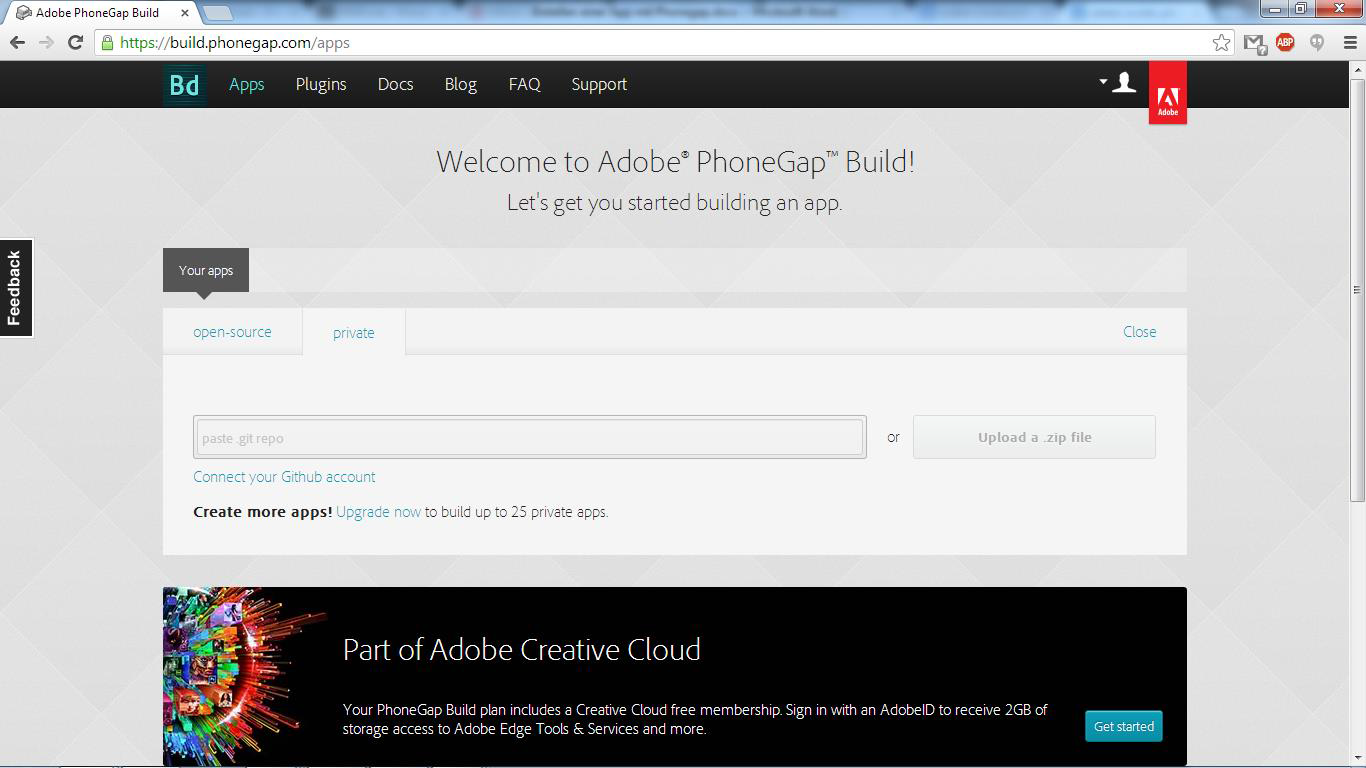
\includegraphics[keepaspectratio=true, width=14cm]{images/phoneGap/PhoneGap1.png}
\caption{PhoneGapwebsite vom 21.04.2014}
\end{figure}

Hier muss man nun den Reiter \enquote{private} auswählen, damit man die Appdaten in Form eines Zipfiles hochladen kann.
Um Fortzufahren, muss man nun das Zipfile, in welchem die Daten für die App(alle HTML, CSS und JavaScript-Files) gespeichert sind, hochladen.\\
Ist das geschehen, versucht die Webseite die Apps für Android, WindowsPhone und iOS zu compilieren. Für Android und WindowsPhone funktioniert das auch, falls der Code und vor allem die Konfigurationsdatei korrekt sind, aber bei iOS kommt eine Fehlermeldung. Denn um Apps für iOS zu erstellen benötigt man Zertifikate, welche man nur als Apple-Developer bekommt.\\
Nach dem ersten Build sieht man, dass für den Appnamen das Appsymbol und weitere Einstellungen die Einstellungen aus der config.xml übernommen wurden.\\

\begin{figure}[H]
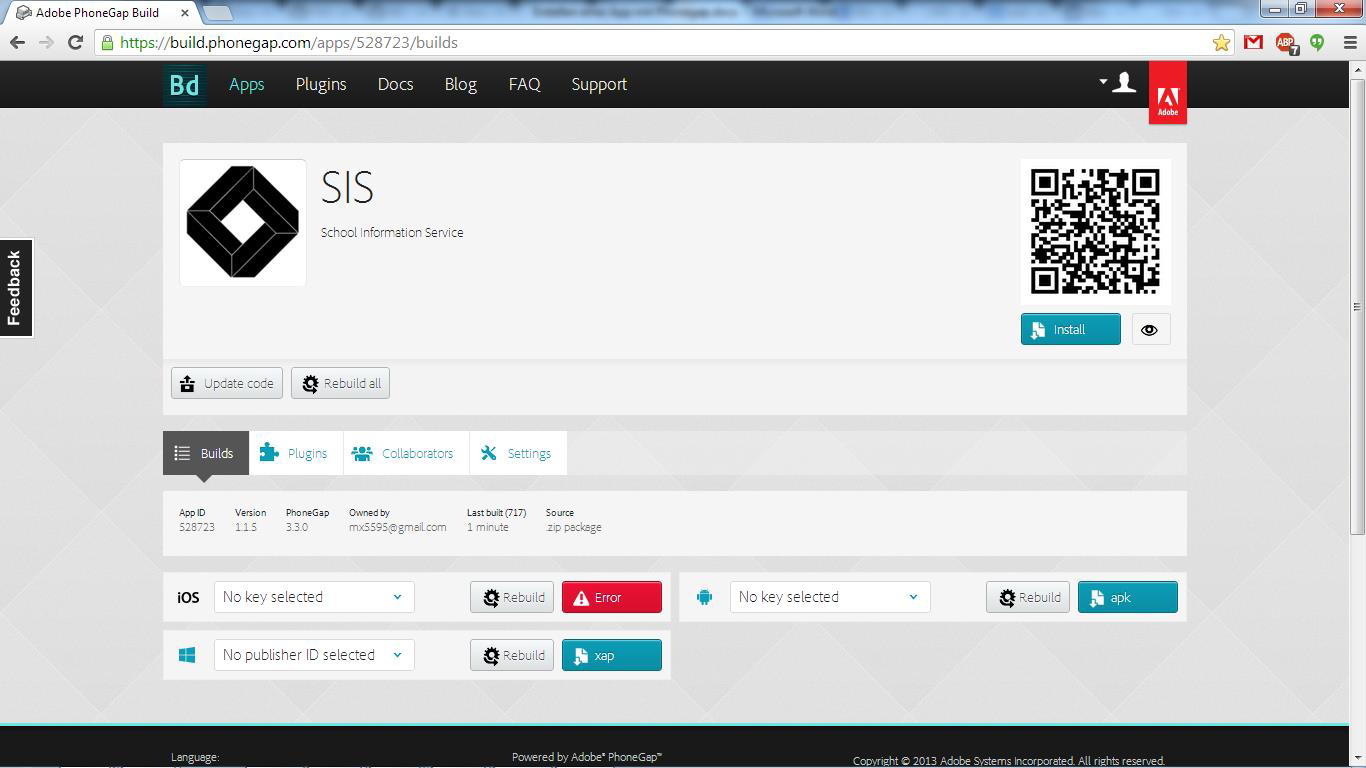
\includegraphics[keepaspectratio=true, width=14cm]{images/phoneGap/PhoneGap2.png}
\caption{PhoneGapwebsite vom 21.04.2014}
\end{figure}

Um die Applikation zu updaten, müssen alle Dateien die verändert wurden in der ZIP-Datei ausgetauscht werden und die ZIP-Datei muss neu hochgeladen werden. Dazu klickt man einfach auf \enquote{Update code} und wählt dann die gewünschte ZIP-Datei aus.\\
Die Android-App und die App für WindowsPhone kann man jetzt bereits testen. Bei Android muss man dazu nur zuerst in den Einstellungen, im Untermenü Anwendungen, die Option \enquote{Unbekannte Quellen} aktivieren. Dann kann man einfach das APK-File auf das Gerät laden(entweder direkt mit dem Gerät downloaden oder via USB, Bluetooth, etc. auf das Gerät laden) und ausführen, und die Applikation wird wie jede andere App installiert. Nun kann man die App nutzen.\\
Die App auf dem WindowsPhone zu nutzen ist etwas umständlicher. Entweder man stellt die App direkt in den Store oder wenn man sie nur testen möchte, kann man die App auch mit Hilfe von Developer Tools direkt auf das Smartphone laden und testen.\\
Damit die Android-App in den Play-Store von Google geladen werden kann, muss diese zuerst noch signiert werden. Dazu muss eine Keystore-Datei erzeugt werden, mit welcher die App signiert werden kann.\\
Dieses Keystore-File kann man selbst erstellen, sofern man die JDK (Java Development Kit) installiert hat. Um den Schlüssel zu erstellen muss man die Eingabeaufforderung öffnen und in das Verzeichnis der JDK wechseln, als nächstes kann man mit dem Befehl keytool und einigen Parametern ein Keystotre-File erstellen.\\
Beispielbefehl:\\

\begin{lstlisting}
$ keytool -genkey -v -keystore my-release-key.keystore -alias alias_name -keyalg RSA -keysize 2048 -validity 10000
\end{lstlisting}

Nachdem dieser Befehl eingegeben wurde, wird man noch aufgefordert, den Namen des Entwicklers oder Entwicklerteams, die Nationalität und einige weiter Angaben einzugeben. Zuletzt muss noch ein Passwort angegeben werden, dieses wird benötigt um den Schlüssel zu entsperren, wenn er bei PhoneGap genutzt wird.\\
Nun wird eine Datei, in diesem Fall mit dem Namen my-release-key.keystore, erstellt.\\
Wenn man nun das Dropdownmenü neben dem Androidsymbol öffnet,\\


\includegraphics[keepaspectratio=true, width=7cm]{images/phoneGap/PhoneGap3.png}

erscheint ein Punkt \enquote{add a key…}. Wenn man diesen Punkt auswählt wird man aufgefordert eine Datei hochzuladen, dabei handelt es sich um die Keystore-Datei, welche zuvor erzeugt wurde. Dann muss man dem Schlüssel noch einen Namen geben und bestätigen.\\
Nun kann man in diesem Dropdownmenü den hochgeladenen Schlüssel auswählen, um ihn zu nutzen muss man zuerst noch ein Passwort eingeben, das ist jenes Passwort welches zuvor beim erstellen des Keystore-Files angegeben wurde. Wenn man nun einen Rebuild macht, bekommt man eine Android-Release-App, welche auch im Play-Store veröffentlicht werden kann.
Bei iOS benötigt es bereits ein Entwicklerzertifikat, um eine Debug-App zu erstellen. Um ein solches Zertifikat zu erstellen muss man bei Apple als Developer angemeldet sein und 99\$ im Jahr bezahlen.\\
Für dieses Projekt wurde der Apple-Enterprise-Account der Schule genutzt. Man benötigt nur eine Apple ID (Registrierung unter https://developer.apple.com/register/ ), mit dieser kann man dann von einem Administrator (in unserem Fall Direktor Laner) zum Account hinzugefügt werden.\\
Nachdem man zum Enterprise-Programm hinzugefügt wurde, muss man das MemberCenter (https://developer.apple.com/membercenter/ ) öffnen.\\

\begin{figure}[H]
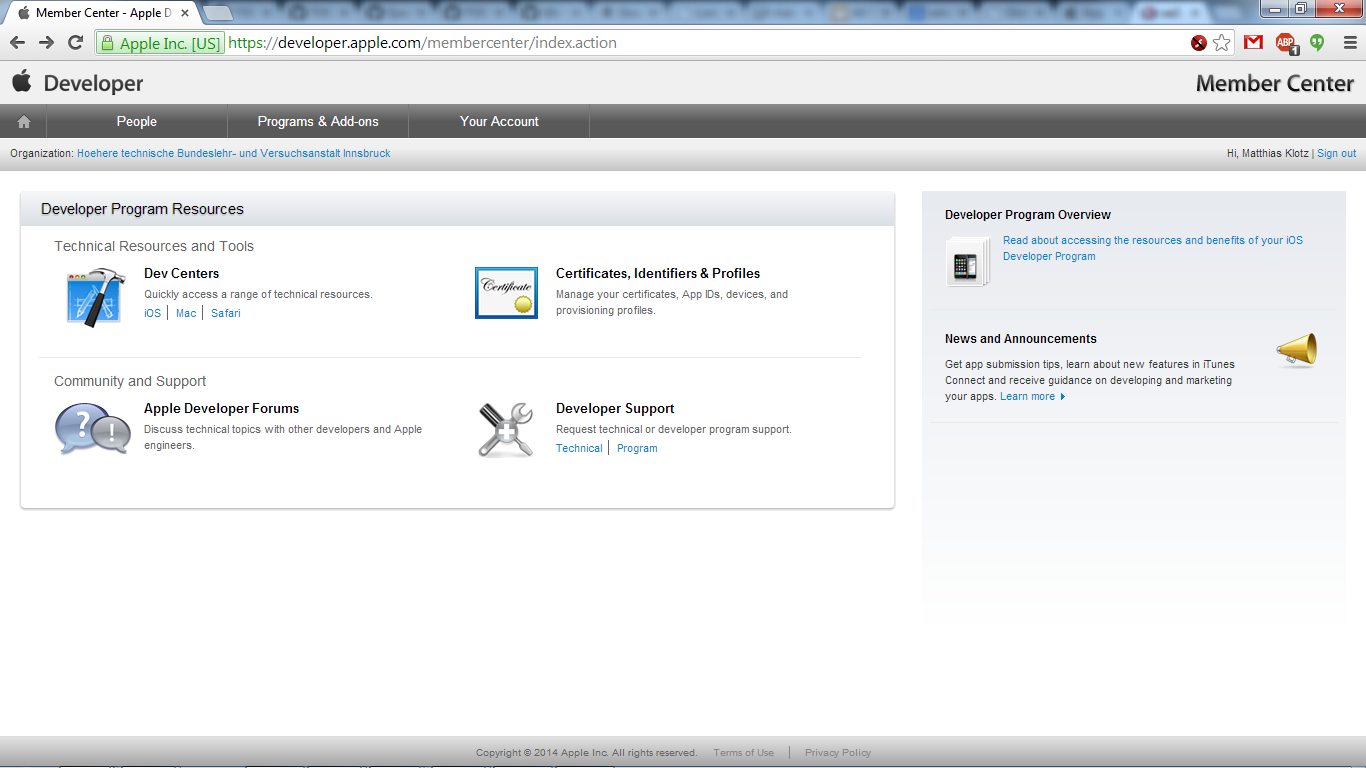
\includegraphics[keepaspectratio=true, width=14cm]{images/phoneGap/AppleMemberCenter1.png}
\caption{Applewebsite vom 21.04.2014}
\end{figure}

Unter \enquote{Certificates, Indentifiers \& Profiles} kann man nun die benötigten Zertifikate erstellen und downloaden.\\

\begin{figure}[H]
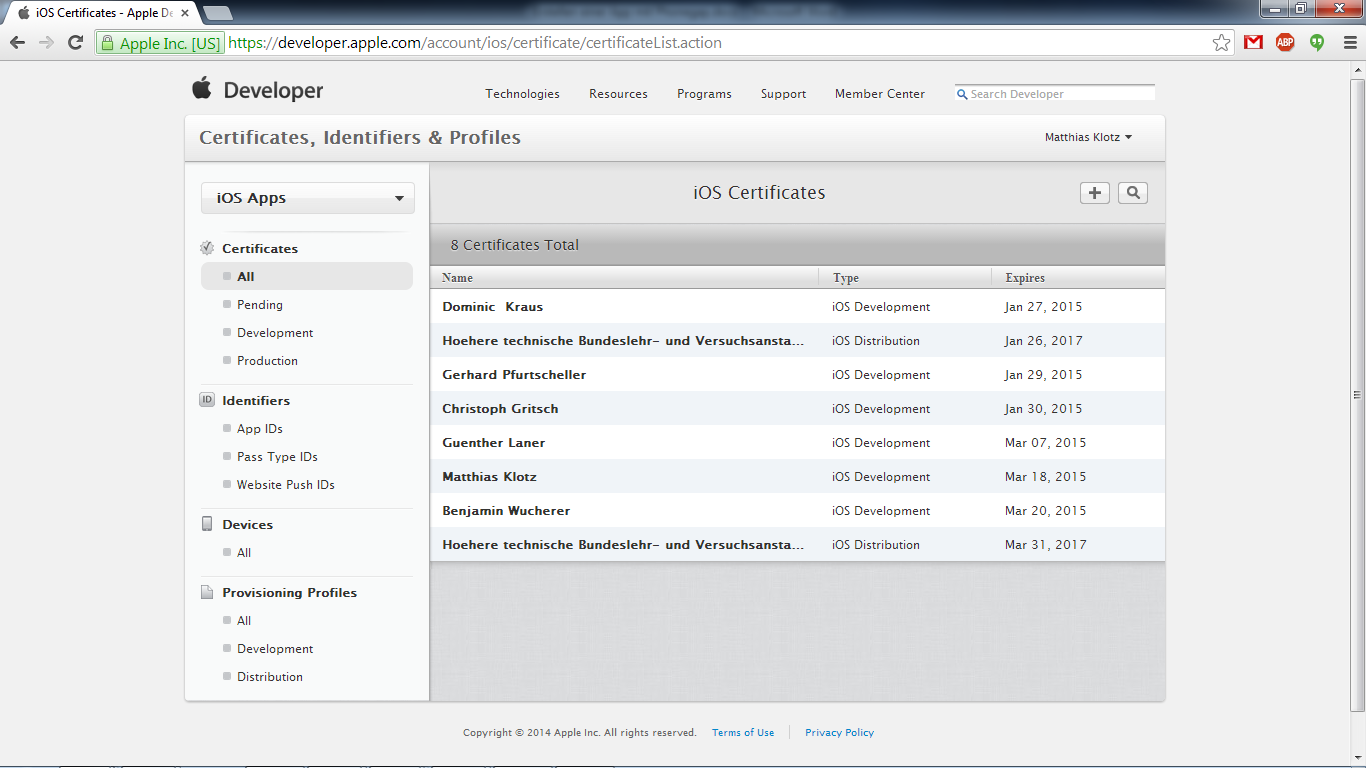
\includegraphics[keepaspectratio=true, width=14cm]{images/phoneGap/AppleMemberCenter2.png}
\caption{Applewebsite vom 21.04.2014}
\end{figure}

Um ein neues Zertifikat zu erstellen, öffnet man zuerst den Menüpunkt Certificates und klickt dann auf das Plus-Symbol in der rechten oberen Ecke des Fensters. Daraufhin erscheint der Assistent zum erstellen eines neuen Zertifikates.
Als erstes wird gefragt wozu das Zertifikat verwendet wird. Dabei muss man zuerst unterscheiden ob es sich um ein Development oder ein Production Zertifikat handelt. Bei einem Development Zertifikat
werden bestimmte Developergeräte angegeben, auf welchen die Applikation getestet werden kann, ohne dass sich die App im Appstore befindet.\\
Ein Production Zertifikat wird hingegen benötigt, um eine App zu erstellen, welche für alle Geräte nutzbar ist, diese App muss dann aber für gewöhnlich über den Appstore veröffentlicht werden.\\
Für dieses Projekt wurden beide Varianten erstellt und genutzt.\\
Bei beiden Varianten wird man im nächsten Schritt aufgefordert einen CSR (Certificate Signing Request) hochzuladen. Diese \enquote{Datei} erhält man indem man die Schlüsselbundverwaltung bei Mac OS X öffnet und im Menü Datei unter Zertifikats Assistent, \enquote{neues Zertifikat erstellen} wählt. Dabei wird man aufgefordert eine E-Mail-Adresse und den eigenen Namen anzugeben, wichtig ist das der Punkt als Datei speichern ausgewählt wird.\\
Nach Angabe der Informationen kann man nun eine CSR-Datei abspeichern. Diese Datei wird als nächstes bei der Erstellung des Zertifikates auf der Apple-Website hochgeladen. Nun kann man das Zertifikat erstellen und downloaden.
Als nächstes muss noch ein Provisoining-File erstellt werden. Dazu wechselt man einfach auf den Menüpunkt Provisioning Profiles und klickt dann auf das selbe Symbol wie zuvor bei den Zertifikaten. Es erscheint wieder ein Assistent, der bei der Erstellung des Provisioning Profils hilft. Als erstes muss man wieder angeben wozu das Provisioning Profile benötigt wird. Wenn man zuvor ein Development Zertifikat erstellt hat, muss man nun wieder Development auswählen, hat man aber zuvor ein Production Zertifikat erstellt, muss man nun Distribution auswählen. Im nächsten Schritt muss noch eine App-ID gewählt werden, dazu wurde einfach eine bereits existierende ID ausgewählt. Als nächstes wird nach einem Zertifikat gefragt, hier wird das zuvor erstellte Zertifikat ausgewählt.\\
Falls ein Development Provisioning Profile erstellt wird, wird man noch nach den Entwicklergeräten gefragt, hier muss man sein eigenes iPhone, welches zuvor unter Devices hinzugefügt wurde, auswählen.\\
Wenn man soweit ist kann man auch das Provisioning Profile generieren und herunterladen.\\
Da für PhoneGap aber ein privater Schlüssel in Form eines P12-Files benötigt wird, muss dieser erst aus dem Zertifikat exportiert werden. Dazu muss man zuerst das heruntergeladene Zertifikat in die Schlüsselbundverwaltung importieren, dann wählt man das soeben importierte Zertifikat aus, nun klickt man mit der rechten Maustaste darauf und wählt exportieren aus und exportiert das Zertifikat als P12-Datei.\\
\\
Wenn man nun das Dropdownmenü neben dem Apple-Logo öffnet,

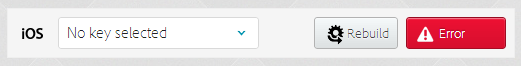
\includegraphics[keepaspectratio=true, width=7cm]{images/phoneGap/PhoneGap4.png}

erscheint ein Punkt \enquote{add a key…}. Wenn man diesen Punkt auswählt wird man aufgefordert zwei Dateien hochzuladen, eine P12-Datei und ein Provisioning-File, dabei handelt es sich um die beiden Dateien die gerad erstellt wurden. Wenn diese Dateien hochgeladen wurden kann die Applikation erstellt werden.\\
Hat man ein Developer-Zertifikat erstellt, kann die erstellte App nur auf den in dem Zertifikat bestimmten Geräten betrieben werden, wurde aber ein Distribution Zertifikat erstellt, kann die App nun auf allen iOS-Geräten verwendet werden.\\
Um die App für den App-Store zu builden, wurden uns die Zertifikate von Direktor Günther Laner zur Verfügung gestellt, da die Applikation über den Developer Account des Direktors veröffentlicht wird.\\

% Söö: Wie wurde die App erstellt?
% Ich weiß das leider nicht so genau, deswegen kann ich dir nicht vorschlagen, was du erwähnen sollst, und was nicht. 
% Die Generierung des Stunden- und Supplierplans musst du nicht mehr erwähnen.
% 
% Hier dürfen auch auch Sourcecode-Teile vorkommen.
% Wenn Sourcecodes: jeweilge File in den Ordner /sources/ in einen Unterordner packen und mit folgendem Befehl includieren:
%
%
% \lstinputlisting[style=custom, language=php, caption={Dateiname}, label={lst:content_imple_timetables_labelname}]{sources/ordner/datei.php}
%
% Als weitere Eigenschaft kannst du die Zeilen angeben: [firstline=300, lastline=500]
% Damit nicht alles reinkopiert wird.
\newpage

\subsection{Designs}
\subsubsection{Menü}
Die Generierung des Menüs erfolgt in der Datei /modules/menu/Main.php.\\
\paragraph{Aufbau der Seite\\}
Wie bereits unter \gref{sec:content_draft_design_web} erwähnt, besteht das Design des Menüs grundsätzlich aus dem SIS-Logo in der Mitte und links und rechts davon, in zwei Zeilen gruppiert, vier Plätze für Menüpunkte, die je nach Bedarf aus- und eingeblendet werden.\\
\\
Diese Menüpunkte sind nach zwei verschiedenen Systemen ansprechbar.\\
Die programmiertechnisch einfachere Methode ist die, dass alle Punkt durchnummeriert werden (siehe \autoref{fig:content_imple_menu_layout1}).\\ Diese Methode ist serverseitig (PHP) die wichtigere.
\begin{figure}[H]
\centering
\resizebox{16cm}{!}{
    \fdot[scale=1]{images/design-layout1}{}
}
\caption{Menü: Seiten-Layout, Nummerierung}
\label{fig:content_imple_menu_layout1}
\end{figure}
Die zweite Methode, um die Menüpunkte anzusprechen, ist der logische, strukturelle Aufbau, und die daraus resultierte Struktur, aus der sich eine Nomenklatur für die Punkte ergibt (siehe \autoref{fig:content_imple_menu_layout2}).\\
Man unterteilt zunächst zwischen der oberen Reihe (\texttt{menuUp}, in der Grafik abgekürzt mit U) und unterer Reihe (\texttt{menuDown}, in der Grafik abgekürzt mit D).\\
Weiters wird zwischen linkem und rechtem Menü-Block (in der Grafik durch L beziehungsweise R abgekürzt).\\
Als letztes wird noch zwischen in innen- und außenliegenden Menüpunkten unterschieden, diese Eigenschaft wird \enquote{Level} genannt (innenliegende Punkte sind Level 1 - abgekürzt L1 - außenliegende sind Level 2 - abgekürzt L2). Für die Implementierung wurden die letzten zwei Unterscheidungsstufen zusammengefügt.\\
Es ergeben sich dadurch folgende Unterscheidungen:
\begin{itemize}
	\item \texttt{menuLeftLevel1}
	\item \texttt{menuLeftLevel2}
	\item \texttt{menuRightLevel1}
	\item \texttt{menuRightLevel2}
\end{itemize}
Diese Methode ist clientseitig wichtiger, da JavaScript durch DOM im Gegensatz zu PHP auf die HTML-IDs und HTML-Klassen zugreifen kann.
\begin{figure}[H]
\centering
\resizebox{16cm}{!}{
    \fdot[scale=1]{images/design-layout2}{}
}
\caption{Menü: Seiten-Layout, logische Nomenklatur}
\label{fig:content_imple_menu_layout2}
\end{figure}

\paragraph{Konfiguration des Menüs\\}
Wenn das Modul geladen wird (durch das \texttt{include()}-Kommando), so wird es automatisch initialisiert. Initialisierung ist dabei so zu verstehen, dass die nötigen globalen Variablen, die zur Konfiguration dienen, definiert werden.\\
\lstinputlisting[style=custom, language=php, caption={/modules/menu/Main.php; Initialisierung; Zeilen 3-19}, label={lst:content_imple_menu_global}, firstline=3, lastline=19, firstnumber=3]{sources/menu/Main.php}
Erklärung der globalen Variablen:\\
\begin{table}[H]
\centering
\begin{tabular}{p{2.5 cm}p{11 cm}}
	\toprule
		\textbf{Variable} & \textbf{Bedeutung} \\
	\midrule
		\texttt{\$back} & Link zur vorigen Seite; Wird bei Klick auf das Logo oder den Text links oben geöffnet.\\
		\hline
		\texttt{\$headerText} & Text, der oben links angezeigt werden soll.\\
		\hline
		\texttt{\$name} & $ \widehat{=} $ Benutzername. Wird oben rechts angezeigt.\\
		\hline
		\texttt{\$buttons} & Numerisches Array mit 8 Einträgen (0 bis 7, für die jeweiligen Buttons), jeder Eintrag ist ein assozitives Array (für die Schüssel, siehe \autoref{tab:content_imple_design_menu_buttons})\\
	\bottomrule
\end{tabular}
\caption{Globale Konfiguration des Hauptmenüs}
\label{tab:content_imple_design_menu_global}
\end{table}

Die Einträge im Array \texttt{\$buttons} haben folgende Schlüssel:\\
\begin{table}[H]
\centering
\begin{tabular}{p{2.5 cm}p{11 cm}}
	\toprule
		\textbf{Schlüssel} & \textbf{Bedeutung} \\
	\midrule
		\texttt{displayed} & Soll der entsprechende Menüpunkt angezeigt werden?\\
		\hline
		\texttt{enabled} & Darf der Benutzer den Punkt benutzen?\\
		\hline
		\texttt{svg} & Link zur Grafik des Menüentrags (muss als SVG-Datei vorliegen); \newline
			\textit{Beachte:} Link muss absolut sein.\newline
			\textit{Beispiel:} \texttt{ROOT\_LOCATION . "/data/images/base.svg";}
			\\
		\hline
		\texttt{text} & Dieser Text wird unter der Grafik angezeigt.\\
		\hline
		\texttt{jsurl} & Link des Menüpunktes; Wo kommt man hin, wenn man auf den Punkt klickt?\\
		\hline
		\texttt{url} & Analog zu \texttt{jsurl}; Dieser Wert wird verwendet, wenn kein JavaScript zur Verfügung steht.\\
	\bottomrule
\end{tabular}
\caption{Globale Konfiguration des Hauptmenüs; Fortsetzung}
\label{tab:content_imple_design_menu_buttons}
\end{table}
Diese gloabel Konfigurationsfelder können/müssen durch den Benutzer verändert werden, um das Menü anzupassen.\\
Die zwei Konstanten \texttt{BASE\_RL} und \texttt{BASE\_LR} referenzieren absolut auf zwei Graphiken (siehe später).
\newpage
\paragraph{Ausgabe\\}
Die Ausgabe des Menüs ist eigentlich ziemlich trivial, es sollen hier nur die interessanten Teile näher betrachtet werden.\\
Um die HTML-Struktur der unter logischen und numerischen Identifizierung der Menüteile anzupassen, wurde vereinfacht gesprochen folgender Aufbau verwendet (es wird nur Knoten unterhalb des \texttt{body}-Tags berücksichtigt):
\begin{lstlisting}[style=custom, language=html,  caption={Grundsätzliche HTML-Struktur der Menüs},label={lst:content_imple_design_htmlstruct}]
<div id="header">
	<div id="title">
		<!-- Hier ist der Titel der Seite -->
	</div>
	<div id="userInfo">
		<!-- Hier ist der Benutzername und der "Abmelden"-Button -->
	</div>
</div>
<div id="menuContainer">
	<div id="menuUp">
		<div  class="mid">
			<!-- Hier ist der obere Teil des Logos -->
		</div>
		<div class="menuRightLevel1">
			<!-- Das ist Menuepunkt 2 -->
			<!-- Hier wird das entsprechende Bild eingebunden -->
			<div class="subtext">
				<!-- Hier steht der Text des Menuepunktes -->
			</div>
		</div>
		<div class="menuRightLevel2">
			<!-- Das ist Menuepunkt 3 -->
			<!-- Hier wird das entsprechende Bild eingebunden -->
			<div class="subtext">
				<!-- Hier steht der Text des Menuepunktes -->
			</div>
		</div>
		<div class="menuLeftLevel2">
			<!-- Das ist Menuepunkt 0 -->
			<!-- Hier wird das entsprechende Bild eingebunden -->
			<div class="subtext">
				<!-- Hier steht der Text des Menuepunktes -->
			</div>
		</div>
		<div class="menuLeftLevel1">
			<!-- Das ist Menuepunkt 0 -->
			<!-- Hier wird das entsprechende Bild eingebunden -->
			<div class="subtext">
				<!-- Hier steht der Text des Menuepunktes -->
			</div>
		</div>
	</div>
	<!-- Hier wuerde noch der entsprechende Code für die untere Haelfe kommen -->
	</div>
</div>
\end{lstlisting}
Das Beispiel unter \autoref{lst:content_imple_design_htmlstruct} ist natürlich nicht vollständig. Allerdings soll es den prinzipiellen Aufbau zeigen. An der Stelle des Kommentares über die untere Hälfte, steht nochmal der Code der oberen Hälfte, nur, dass die ID des Divs nun \texttt{menuDown} lauten würde und die Punkte haben selbstverständlich andere Nummern.\\
\\
\newpage
Bei der Betrachtung fällt auf, dass der obere und der untere Teil des Logos getrennt eingebunden ist. Dies ist begründet dadurch, dass, wie bereits unter \gref{sec:content_draft_design_web} erwähnt wurde, das Logo bei Klick auf einen Menüpunkt in einer Animation auseinanderfahren soll. Dies ist am leichtesten möglich, indem man das Bild in zwei Sub-Bilder aufteilt. Das Logo wurde allerdings nicht willkürlich zerteilt, sondern wurde anhand der Kanten zerschnitten, was bei den Animationen dann letzten Endes schöner wirkt (siehe \autoref{fig:content_impl_design_logo-down} und \autoref{fig:content_impl_design_logo-down}).\\
\begin{figure}[H]
	\centering
	\begin{minipage}{7cm}
		\centering
		
\includegraphics[keepaspectratio=true, height=5cm]{images/logo-black.png}
		\caption{Logo, vollständig}
		\label{fig:content_impl_design_logo}
	\end{minipage}
\end{figure}

\begin{figure}[H]
	\centering
	\begin{minipage}{7cm}
		\centering
		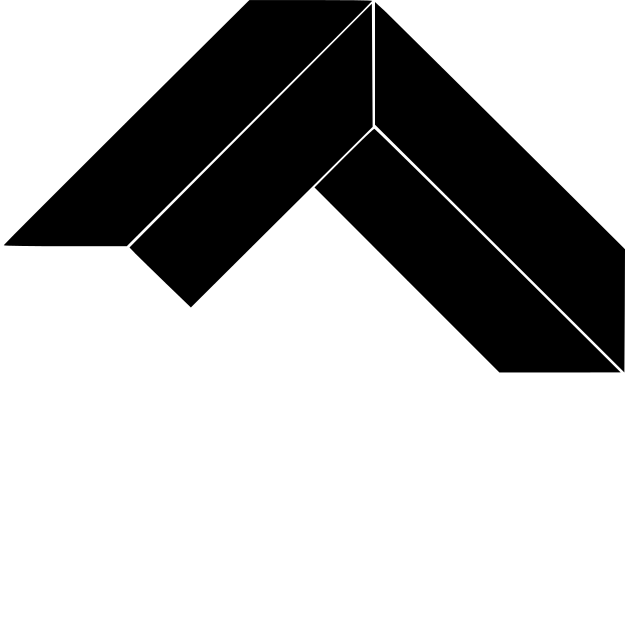
\includegraphics[keepaspectratio=true, height=5cm]{images/logo-up.png}
		\caption{Logo, oberer Teil}
		\label{fig:content_impl_design_logo-up}
	\end{minipage}
	\hspace{1cm}
	\begin{minipage}{7cm}
		\centering
		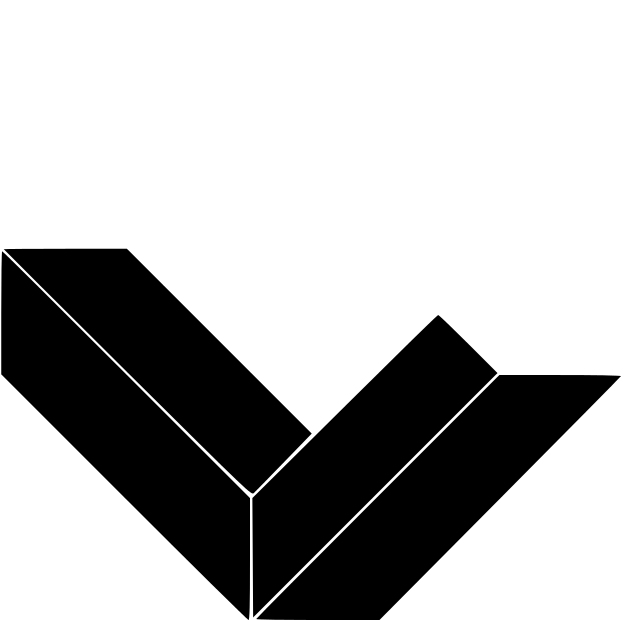
\includegraphics[keepaspectratio=true, height=5cm]{images/logo-down.png}
		\caption{Logo, unterer Teil}
		\label{fig:content_impl_design_logo-down}
	\end{minipage}
\end{figure}
Die Ausgabe der Menüpunkte (\autoref{lst:content_imple_design_htmlstruct}) soll nun am Beispiel des Punktes 2 (dies entspricht dem ORL1) näher erläutert werden.\\

\newpage

\lstinputlisting[style=custom, language=php, caption={/modules/menu/Main.php; Bespiel: Menüpunkt 2; Zeilen 65-78}, label={lst:content_imple_menu_2}, firstline=65, lastline=78, firstnumber=65]{sources/menu/Main.php}
Der Div, der den Menüpunkt umschließt, bekommt die HTML-Klasse \texttt{notUsed} angehängt, im Fall, dass der Wert des \texttt{display}-Schlüssels für den Punkt 2 \texttt{false} ist. Diese Klasse blendet im Grund den Div aus.\\
Kann der Button verwendet werden - also wenn sein \texttt{enabled}-Schlüssel auf \texttt{true} (technisch gesehen ist hier jeder Wert außer 0 gültig, aber logisch ist es entweder \texttt{true} oder \texttt{false}) gesetzt ist - so wird die Ziel-URL des Links in einen Div-Tag der Klasse \texttt{linkAdr} (Elemente dieser Klasse sind nicht sichtbar) geschrieben. Später wird via JavaScript der Link aus diesem Div ausgelesen und die \texttt{onclick}-Events für das Bild und den Text darunter neu gesetzt.\\
In Zeile 71 wird die Grafik, die durch die Konstante \texttt{BASE\_LR} referenziert wird, eingebunden. Diese Graphik hat die selbe Parallelprogramm-Form, wie die Grafiken der Menüpunkte, jedoch durchgehend, ohne Muster. Sämtliche Mouse-Events werden über diese einheitlichen Grafiken ausgelöst, da sonst in den leeren Bereichen keine Events getriggert werden können (Der gleiche Effekt wird als Vorteil genutzt und war der Hauptgrund, warum man auf SVG-Grafiken zurückgegriffen hat $ \Longrightarrow $ Es ist mit ihnen möglich, nicht-rechteckige Bereiche mit Mouse-Events zu versehen.). Damit diese homogenen Grafiken nicht das Bild zerstören, wurde ihre Tranzparenz mittels CSS auf einen sehr hohen Wert gestellt $ \Longrightarrow $ Diese Grafiken sind nicht sichtbar.\\
In der nächsten Zeile wird die eigentliche Grafik ausgegeben. Damit die zwei SVG-Elemente am Schluss genau übereinander liegen, wurden ihre \texttt{position}-Attribute mit CSS auf \texttt{absolute} gestellt.\\
Im Div mit der Klasse \texttt{subtext} wird nun der Link erstellt. Als \texttt{href}-Attribut hat er die Nicht-JavaScript-URL. Damit, im Falle dass JavaScript aktiviert ist, die richtige URL geöffnet wird, wird später das \texttt{onclick}-Event dementsprechend modifiziert (Wichtig ist hierbei, dass die Funktion des Events \texttt{false} zurückgibt, ansonsten würde die Standard-Aktion weiter ausgeführt - also in diesem Fall das öffnen des Nicht-JavaScript-Links.).\\
Die anderen Menü-Punkte sind analog.\\
\paragraph{JavaScripts\\}
Die im Menü verwendeten Scripts sind größtenteils trivial.\\
Es werden folgende Funktionen definiert:
\begin{table}[H]
\centering
\begin{tabular}{p{3.5 cm}p{11 cm}}
	\toprule
		\textbf{Funktion} & \textbf{Bedeutung} \\
	\midrule
		\texttt{main()} & Wird beim Laden der Seite ausgeführt. Setzt die \texttt{onclick}-, \texttt{onmouseenter}- und \texttt{onmouseleave}-Events der Grafiken und Links.\\
		\hline
		\texttt{openLink(link)} & Öffnet den als Parameter angegebenen Link mit Animation in einem neu-erstellten iFrame. Ist bereits ein Link geöffnet, so wird dieser zuvor geschlossen. Hat der zu öffnende Link einen GET-Parameter \textit{menu}, so wird der Link nicht im iFrame geöffnet, sondern normal. Hat der Link einen Fragmentbezeichner, so wird dieser beim Öffnen entfernt und im Scope des iFrames die Funktion \texttt{smoothScroll()} aufgerufen (Diese ist in der Datei /data/scripts/main.js definiert). Das \texttt{onclick}-Event des Close-Buttons im iFrame wird so modifiziert, dass bei Klick ist \texttt{closeLink()}-Funktion des drüberliegenden Frames ausgeführt wird.\\
		\hline
		\texttt{closeLink()} & Fährt die Animation wieder rückfährts ein.\\
		\hline
		\texttt{hoverLink(half, row)} & Ändert die Farbe der Grafik des Menüeintrages, der durch die Parameter identifiziert ist, auf einen hellen Grauwert (\texttt{\# ccc}). Und die Textfarbe des Namens des Punktes auf schwarz.\\
		\hline
		\texttt{dehoverLink(half, row)} & Ändert die Farbe der Grafik des Menüeintrages, der durch die Parameter identifiziert ist auf schwarz. Und die Textfarbe des Namens des Punktes auf weiß.\\
		\hline
		\texttt{hoverLinkMiddle()} & Ändert die Farbe der Grafik des Logos auf einen hellen Grauwert (\texttt{\#ccc}).\\
		\hline
		\texttt{dehoverLinkMiddle()} & Ändert die Farbe der Grafik des Logos auf schwarz.\\
		\hline
		\texttt{checkMobile()} & Leitet, wenn es sich um einen mobilen Webbrowser handelt, auf die Mobilseite um. Diese Funktion wird nicht ausgeführt, wenn der GET-Parameter \texttt{noMobile} angegeben wird.\\
	\bottomrule
\end{tabular}
\caption{JavaScript-Funktionen für Menü}
\label{tab:content_imple_design_menu_script_functions}
\end{table}
Bei der Implementierung dieser Funktionen gibt es eigentlich keine Herausforderungen. Für den Quellcode siehe \gref{sec:content_imle_source}.

\subsubsection{Designs via Managementsystem}
Da ja bereits unter \gref{sec:content_imple_base_site} ausführlich auf das Management von Designs eingegangen wurde, soll nun nur noch anhand eines Beispiels der Aufbau eines Designs, die Verwendung mit dem Design-Management-System und grundsätzliche Design-Richtlinien erklärt werden.\\
Als Beispiel wird das Design \enquote{supmain} (/modules/design/submain.html) verwendet.
\lstinputlisting[style=custom, language=php, caption={/modules/designs/supmain.html}, label={lst:content_imple_design}]{sources/design/supmain.html}
Es handelt sich im Wesentlichen um eine Standard-HTML-Datei. Die aktuell interessantesten Teile der Datei sind die Platzhalter.\\
Der erste befindet sind in Zeile 10: Es handelt sich um den Platzhalter für Titel der Seite. Das bedeutet, dass, wenn mit diesem Design eine Seite mit dem Titel \enquote{Testseite} geladen wird, der Text in der Fenster-Titel-Leiste \enquote{SIS.Web Access - Testseite} lautet.\\
In den Zeilen 11 bis 15 ist der Platzhalter \texttt{\&root;} zu sehen. Dieser wird beim Laden des Designs durch den Pfad zum Projekt-Grundverzeichnis relativ zum Document-Root des Webservers ersetzt.\\
An der Stelle des, in Zeile 38 vorkommenden, Platzhalters wird der Text der Website eingefügt.\\
\\
In diesem Beispiel sind noch die beiden Scripts in den Zeilen 4 bis 9 und 16 bis 25 interessant. Das erste versucht zu erkennen, ob die Seite in einem Frame geladen wird, und springt aus dem Frame in den drüber liegenden. Das Zweite prüft, im Falle dass der durch den Platzhalter \texttt{\&mobile;} eingesetzte Wert nicht \texttt{false} ist, ob ein mobiler Webbrowser verwendet wird, und leitet ihn auf die mobile Seite um. Die Funktion, die mobile Browser erkennt \texttt{isMobile()} wird in der Datei /data/scripts/miscellaneous.js definiert.\\
\\
Das soeben erläuterte Design wird unter anderem für Login verwendet. Der Name \enquote{supmain} steht für \enquote{super Main}, also \enquote{über Main}, rührt daher, dass das Design für die in das Menü mit iFrames eingebetteten Seiten das Design \enquote{main} verwenden. Da das besprochene Design dem des Menüs ähnelt, also quasi \enquote{über dem main-Design} liegt, wurde ein passender Name schnell gefunden. 

\subsection{Probleme während der Implementierung}
% Sind bei irgendwem Probleme bei der Entwicklung aufgetreten?
% Die Frage war rhetorisch, natürlich sind.
% Wenn ihr was dazu schreiben wollt, dann kommentiert auf diesem commit auf github. Ich füge dann eine neue Datei hinzu und füge sie hier ein.
%
% Ah und: Sry, wegen der vielen E-Mails, aber ich habe den Eindruck, wenn jeder genau weiß, was er machen muss, geht es schneller voran. : )#

\subsection{Sourcecode}
\label{sec:content_imle_source}

Der vollständige Sourcecode (Stand: ) // TODO
ist auf der angehängten CD zu finden.

\subsection{Test- Und Messergebnisse}
